\begin{frame}
	\frametitle{Warm-up}

	What are the following sets?

	\begin{enumerate}
		\item $[2,4] \cup (2,5)$

		\item $[2,4] \cap (2,5)$

		\item $[\pi,e]$

		\item $[0,0]$

		\item $(0,0)$
	\end{enumerate}
\end{frame}

\begin{frame}
	\frametitle{Similar sets}

	What are the following sets?

	\begin{enumerate}
		\item $\displaystyle A = \{ x \in \mathbb{Z}: x^{2}< 6\}$

		\item $\displaystyle B = \{ x \in \mathbb{N}: x^{2}< 6\}$

		\item $\displaystyle C = \{ x \in \mathbb{R}: x^{2}< 6\}$
	\end{enumerate}
\end{frame}

\begin{frame}
	\frametitle{Describing a new set}

	An irrational number is a number that is real but not rational.

	$B$ is the set of positive, rational numbers and negative, irrational numbers.

	Write a definition for $B$ using only mathematical notation. \\ (You may use
	the words ``and", ``or", and ``such that".)
\end{frame}

\begin{frame}
	\frametitle{Sets and quantifiers}

	What are the following sets?

	\begin{enumerate}
		\item $\displaystyle A = \{ x \in \mathbb{R}\, : \, \forall y \in [0,1], \, x
			< y \}$

		\item $\displaystyle B = \{ x \in \mathbb{R}\, : \, \exists y \in [0,1] \text{
			s.t. }x < y \}$

		\item $\displaystyle C = \{ x \in [0,1] \, : \, \forall y \in [0,1], x < y \}$

		\item $\displaystyle D = \{ x \in [0,1] \, : \, \exists y \in [0,1] \text{ s.t.
			}x < y \}$

		\item $\displaystyle E = \{ x \in [0,1] \, : \, \exists y \in \mathbb{R}\text{
			s.t. }x < y \}$

		\item $\displaystyle F = \{ x \in [0,1] \, : \, y \in \mathbb{R}, \, x < y \}$
	\end{enumerate}
\end{frame}

\begin{frame}
	\frametitle{Functions and quantifiers}

	Let $f$ be a function with domain $\mathbb{R}$. Rewrite the following statements
	using $\forall$ or $\exists$:

	\begin{enumerate}
		\item The graph of $f$ intercepts the $x$-axis.

		\item $f$ is the zero function.

		\item $f$ is not the zero function.

		\item $f$ never vanishes.

		\item The equation $\displaystyle f(x)=0$ has a solution.

		\item The equation $\displaystyle f(x)=0$ has no solutions.

		\item $f$ takes both positive and negative values.

		\item $f$ is never negative.
	\end{enumerate}
\end{frame}

\begin{frame}
	\frametitle{Negation 1}

	Write the negation of these statements as simply as possible:

	\begin{enumerate}
		\item My favourite integer number is greater than $7$.

		\item I know at least five students at U of T who have a cellphone.

		\item There is a country in the European Union with fewer than 1000 inhabitants.

		\item All of my friends like apples.

		\item I like apples and oranges.
	\end{enumerate}

	\vfill

	\begin{center}
		Negation of $\displaystyle \boxed{{\color{blue} \cdots}}$ \; = \; $\displaystyle
		\boxed{{\color{blue} \cdots}}$ is false.
	\end{center}
\end{frame}

\begin{frame}
	\frametitle{Negation 2}

	Write the negation of this statement without using any negative words (``no", ``not",
	``none", etc.):

	\begin{quote}
		``\emph{Every page in this book contains at least one word whose first and
		last letters both come alphabetically before M.}''
	\end{quote}
\end{frame}

\begin{frame}
	\frametitle{Negation 3}

	Negate the following statement without using any negative words (``no", ``not",
	``none", etc.):

	\begin{quote}
		``\emph{I have a friend all of whose former boyfriends had at least two
		siblings with exactly three different vowels in their name.}''
	\end{quote}
\end{frame}

\begin{frame}
	\frametitle{Symmetric difference}

	Given two sets $A$ and $B$, we define
	\begin{itemize}
		\item $A \setminus B = \{ x \in A \; : \; x \notin B \}$

		\item $A \triangle B = (A \setminus B) \cup (B \setminus A)$
	\end{itemize}

	\vfill

	Let
	\begin{itemize}
		\item $C_{1}= \{ \text{ students under 18 }\}$

		\item $C_{2}= \{ \text{ students born in Ontario }\}$
	\end{itemize}

	\vfill

	What is the set $C_{1}\triangle C_{2}$?

	\vfill
\end{frame}

\begin{frame}
	\frametitle{Symmetric difference - 2}

	Given two sets $A$ and $B$, we define
	\begin{itemize}
		\item $A \setminus B = \{ x \in A \; : \; x \notin B \}$

		\item $A \triangle B = (A \setminus B) \cup (B \setminus A)$
	\end{itemize}

	\vfill

	Is the following equality
	\[
		(A \triangle B) \triangle C \; = \; A \triangle (B \triangle C)
	\]
	true for all sets $A$, $B$, and $C$?

	\vfill
\end{frame}

\begin{frame}[t]
	\frametitle{Even numbers}

	Write a description of the set $E$ of even integers using set-building
	notation.
\end{frame}

\begin{frame}[t]
	\frametitle{Even numbers}

	Which of these is a correct description of the set $E$ of even integers?
	\begin{enumerate}
		\item $\displaystyle E = \{ n \in \mathbb{Z}\; : \; \forall a \in \mathbb{Z},
			\, n = 2a \}$

		\item $\displaystyle E = \{ n \in \mathbb{Z}\; : \; \exists a \in \mathbb{Z}\text{
			s.t. }n = 2a \}$
	\end{enumerate}

	\vfill
	% \pause

	Which of these statements is true?
	\begin{enumerate}
		\addtocounter{enumi}{2}

		\item $\displaystyle \forall a \in \mathbb{Z}$, the number
			$\displaystyle n=2a$ is even.

		\item $\displaystyle \exists a \in \mathbb{Z}$ s.t. the number
			$\displaystyle n=2a$ is even.
	\end{enumerate}

	\vfill
\end{frame}

\begin{frame}
	\frametitle{Mother}

	Let
	\[
		H = \{ \text{ humans }\}
	\]

	\vfill

	True or False?

	\begin{enumerate}
		\item $\displaystyle \forall x \in H, \; \exists y \in H$ \mbox{ such that }
			$y$ gave birth to $x$

		\item $\displaystyle \exists y \in H \text{ such that }\forall x \in H$, $y$
			gave birth to $x$
	\end{enumerate}

	\vfill
\end{frame}

\begin{frame}
	\frametitle{Elephants}

	True or False?

	\begin{enumerate}
		\item There is a pink elephant in this room.

		\item All elephants in this room are pink.
	\end{enumerate}
\end{frame}

\begin{frame}
	\frametitle{Indecisive function}

	Construct a function $f$ that satisfies all of the following properties at
	once:
	\begin{itemize}
		\item The domain of $f$ is $\mathbb{R}$.

		\item $\displaystyle \forall x \in \mathbb{R}, \exists y \in \mathbb{R}$ such
			that
			\[
				x<y \text{ and }f(x) < f(y)
			\]

		\item $\displaystyle \forall x \in \mathbb{R}, \exists y \in \mathbb{R}$ such
			that
			\[
				x<y \text{ and }f(x) > f(y)
			\]
	\end{itemize}
\end{frame}

\begin{frame}
	\frametitle{ Conditionals - True or False?}

	Let $\displaystyle x \in \mathbb{R}$.

	\begin{enumerate}
		\item $\displaystyle x > 0 \quad \implies \quad x \geq 0$

		\item $\displaystyle x \geq 0 \quad \implies \quad x > 0$

			\vfill
		% \pause

		\item IF $\displaystyle 2 > 3$ THEN Alfonso is in love.
	\end{enumerate}

	\vfill
\end{frame}

\begin{frame}
	\frametitle{Negation of conditionals}

	Write the negation of these statements:
	\begin{enumerate}
		\item If Justin Trudeau has a brother, then he also has a sister.

		\item If a student in this class has a brother, then they also have a sister.
	\end{enumerate}
\end{frame}

\begin{frame}
	\frametitle{Cards}

	Take a look at the following cards.

	\begin{center}
		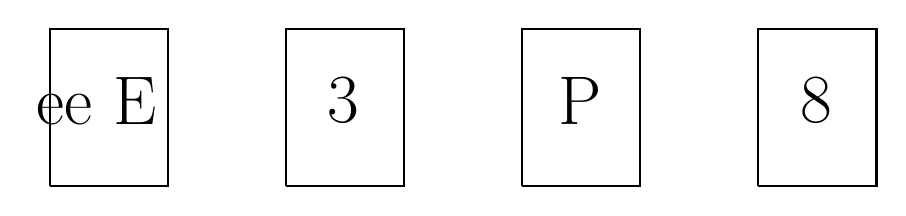
\begin{tikzpicture}
			\draw[thick] (0,0) -- (0,2) -- (1.5,2) -- (1.5,0) -- (0,0);
			\draw[thick] (3,0) -- (3,2) -- (4.5,2) -- (4.5,0) -- (3,0);
			\draw[thick] (6,0) -- (6,2) -- (7.5,2) -- (7.5,0) -- (6,0);
			\draw[thick] (9,0) -- (9,2) -- (10.5,2) -- (10.5,0) -- (9,0);
			\node[below] at (0.6,1.5) {\Huge{\hyperlink{ee}{{ E}} }};
			\node[below] at (3.6,1.5) {\Huge{ 3}};
			\node[below] at (6.6,1.5) {\Huge{ P}};
			\node[below] at (9.6,1.5) {\Huge{ 8}};
		\end{tikzpicture}
	\end{center}

	Each card has a letter on one side and a number on the other, and I tell you:

	\medskip
	\begin{block}{}
		\emph{``\textbf{If} a card has a vowel on one side, \\ \textbf{then} it has an
		odd number on the other side." }
	\end{block}

	\medskip
	Which cards do you need to turn over in order to verify whether I am telling the
	truth or not?

	%

	%

	%%%\Large

	%

	%Four cards lie on the table in front of you.  You know that each card has a letter on one side and a number on the other.  At the moment, you can read the symbols $E$, $P$, $3$, and $8$ on the sides that are up.  I tell you:

	%

	%\vfill

	%

	%\begin{block}{}

	%		 \emph{``\textbf{If} a card has a vowel on one side, \\

	%		 \textbf{then} it has an odd number on the other side." }

	%\end{block}

	%

	%\vfill

	%

	%Which cards do you need to turn over in order to verify whether I am telling the truth or not?
\end{frame}

\begin{frame}
	\frametitle{Cards - 2}

	Four cards lie on the table in front of you. You know that each card has a letter
	on one side and a number on the other.

	{\bfseries Negate} the following statement:
	\begin{block}{}
		\emph{``\textbf{If} a card has a vowel on one side, \\ \textbf{then} it has an
		odd number on the other side." }
	\end{block}
\end{frame}

\begin{frame}
	\frametitle{Hockey}

	Which of the following statements are equivalent to the statement \quad \emph{``Every
	Canadian man likes hockey''}?

	\begin{enumerate}
		\item If a man is Canadian, then he likes hockey.

		\item If a man likes hockey, then he is Canadian.

		\item If a man does not like hockey, then he is not Canadian.

		\item If a man is not Canadian, then he likes hockey.

		\item Non-Canadian men do not like hockey.

		\item If a Canadian does not like hockey, then she is not a man.
	\end{enumerate}
\end{frame}

\begin{frame}
	\frametitle{Graphs}

	Draw the graph of a function $f$ with domain $\mathbb{R}$ that satisfies:
	\begin{equation*}
		\text{If }2<x<4 \text{ then }1<f(x)<2.
	\end{equation*}
	\vfill

	Draw the graph of a function $g$ with domain $\mathbb{R}$ that satisfies:
	\begin{equation*}
		2<x<4 \text{ if and only if }1 < g(x) < 2.
	\end{equation*}
	\vfill
\end{frame}

\begin{frame}
	\frametitle{One-to-one functions}

	Let $f$ be a function with domain $D$. \\

	\vfill

	$f$ is \emph{one-to-one} means that ...
	\begin{itemize}
		\item ... different inputs (${\color{red} x}$) ...

		\item ... must produce different outputs (${\color{red} f(x)}$).
	\end{itemize}

	% \pause
	\vfill

	\begin{block}{}
		Write a formal definition of ``one-to-one".
	\end{block}
\end{frame}

\begin{frame}
	\frametitle{One-to-one functions}

	{\bfseries Definition:} Let $f$ be a function with domain $D$. \\ $f$ is one-to-one
	means ...
	\begin{enumerate}
		\item $\displaystyle f(x_{1}) \neq f(x_{2})$

		\item $\displaystyle \exists x_{1}, x_{2}\in D, \; f(x_{1}) \neq f(x_{2})$

		\item $\displaystyle \forall x_{1}, x_{2}\in D, \; f(x_{1}) \neq f(x_{2})$

		\item $\displaystyle \forall x_{1}, x_{2}\in D, \; x_{1}\neq x_{2}, \; f(x_{1}
			) \neq f(x_{2})$

		\item $\displaystyle \forall x_{1}, x_{2}\in D, \; x_{1}\neq x_{2}\implies f(
			x_{1}) \neq f(x_{2})$

		\item $\displaystyle \forall x_{1}, x_{2}\in D, \; f(x_{1}) \neq f(x_{2}) \implies
			x_{1}\neq x_{2}$

		\item $\displaystyle \forall x_{1}, x_{2}\in D, \; f(x_{1}) = f(x_{2}) \implies
			x_{1}= x_{2}$
	\end{enumerate}
\end{frame}

\begin{frame}
	\frametitle{One-to-one functions}

	Let $f$ be a function with domain $D$. \\ {\bfseries What does each of the following mean?}
	\begin{enumerate}
		\item $\displaystyle f(x_{1}) \neq f(x_{2})$

		\item $\displaystyle \exists x_{1}, x_{2}\in D, \; f(x_{1}) \neq f(x_{2})$

		\item $\displaystyle \forall x_{1}, x_{2}\in D, \; f(x_{1}) \neq f(x_{2})$

		\item $\displaystyle \forall x_{1}, x_{2}\in D, \; x_{1}\neq x_{2}, \; f(x_{1}
			) \neq f(x_{2})$

		\item $\displaystyle \forall x_{1}, x_{2}\in D, \; x_{1}\neq x_{2}\implies f(
			x_{1}) \neq f(x_{2})$

		\item $\displaystyle \forall x_{1}, x_{2}\in D, \; f(x_{1}) \neq f(x_{2}) \implies
			x_{1}\neq x_{2}$

		\item $\displaystyle \forall x_{1}, x_{2}\in D, \; f(x_{1}) = f(x_{2}) \implies
			x_{1}= x_{2}$
	\end{enumerate}
\end{frame}

\begin{frame}
	\frametitle{Proving a function is one-to-one}
	\fontsize{13}{13}\selectfont

	\begin{block}{Definition}
		Let $f$ be a function with domain $D$. \\ We say $f$ is one-to-one when
		\begin{itemize}
			\item \hfill $\displaystyle \forall x_{1}, x_{2}\in D, \; x_{1}\neq x_{2}\implies
				f(x_{1}) \neq f(x_{2})$

			\item OR, equivalently, \hfill $\displaystyle \forall x_{1}, x_{2}\in D, \;
				f(x_{1}) = f(x_{2}) \implies x_{1}= x_{2}$
		\end{itemize}
	\end{block}

	\vfill
	% \pause

	Suppose I give you a specific function $f$ and I ask you to prove it is one-to-one.
	% \pause
	\begin{itemize}
		\item Write the structure of your proof (how do you begin? what do you assume?
			what do you conclude?) if you use the first definition.

		\item Write the structure of your proof if you use the second definition.
	\end{itemize}

	\vfill
	% \pause

	\begin{block}{Exercise}
		Prove that $f(x) = 3x + 2$, with domain $\mathbb{R}$, is one-to-one.
	\end{block}
\end{frame}

\begin{frame}[t]
	\fontsize{13}{13}\selectfont
	\frametitle{Proving a function is NOT one-to-one}

	\begin{block}{Definition}
		Let $f$ be a function with domain $D$. \\ We say $f$ is one-to-one when
		\begin{itemize}
			\item \hfill $\displaystyle \forall x_{1}, x_{2}\in D, \; x_{1}\neq x_{2}\implies
				f(x_{1}) \neq f(x_{2})$

			\item OR, equivalently, \hfill $\displaystyle \forall x_{1}, x_{2}\in D, \;
				f(x_{1}) = f(x_{2}) \implies x_{1}= x_{2}$
		\end{itemize}
	\end{block}

	\vfill
	% \pause

	Suppose I give you a specific function $f$ and I ask you to prove it is not one-to-one.
	% \pause
	You need to prove $f$ satisfies the \emph{negation} of the definition.
	\begin{itemize}
		\item Write the negation of the first definition.

		\item Write the negation of the second definition.

		\item Write the structure of your proof.
	\end{itemize}

	\vfill
	% \pause

	\begin{block}{Exercise}
		Prove that $f(x) = x^{2}$, with domain $\mathbb{R}$, is not one-to-one.
	\end{block}
\end{frame}

\begin{frame}
	\frametitle{Proving a theorem}

	\begin{block}{Theorem}
		Let $f$ be a function with domain $D$.
		\begin{itemize}
			\item IF $f$ is increasing on $\displaystyle D$

			\item THEN $f$ is one-to-one on $\displaystyle D$
		\end{itemize}
	\end{block}

	\vfill
	% \pause

	\begin{enumerate}
		\item Remind yourself of the precise definition of ``increasing" and ``one-to-one".
		% \pause

		\item To prove the theorem, what will you assume? what do you want to show?
		% \pause

		\item Look at the part you want to show. Based on the definition, what is the
			structure of the proof?
		% \pause

		\item Complete the proof.
	\end{enumerate}
\end{frame}

\begin{frame}
	\frametitle{DISproving a theorem}

	\begin{block}{ FALSE Theorem}
		Let $f$ be a function with domain $D$.
		\begin{itemize}
			\item IF $f$ is one-to-one on $\displaystyle D$

			\item THEN $f$ is increasing on $\displaystyle D$
		\end{itemize}
	\end{block}

	\vfill
	% \pause

	\begin{enumerate}
		\item This theorem is false. What do you need to do to prove it is false?
		% \pause

		\item Prove the theorem is false.
	\end{enumerate}
\end{frame}

\begin{frame}
	\frametitle{What is wrong with this proof? (1)}

	\begin{block}{Theorem}
		The sum of two odd numbers is even.
	\end{block}

	% \pause
	\vfill

	\begin{proof}
		3 is odd. \\ 5 is odd. \\ $3+5 = 8$ is even.
	\end{proof}

	\vfill
\end{frame}

\begin{frame}
	\frametitle{What is wrong with this proof? (2)}

	\begin{block}{Theorem}
		The sum of two odd numbers is even.
	\end{block}

	% \pause
	\vfill

	\begin{proof}
		The sum of two odd numbers is always even. \\ even + even = even \\ even +
		odd = odd \\ odd + even = odd \\ odd + odd = even.
	\end{proof}

	\vfill
\end{frame}

\begin{frame}
	\frametitle{Definition of odd and even}

	Write a definition of ``odd integer" and ``even integer".

	% \pause
	\vfill

	\begin{block}{Definition}
		Let $x \in \mathbb{Z}$. We say that $x$ is odd when ...
		\begin{enumerate}
			\item $x = 2a+1$ ?

			\item $\displaystyle \forall a \in \mathbb{Z}, x = 2a+ 1$?

			\item $\displaystyle \exists a \in \mathbb{Z}\text{ s.t. }x = 2a+ 1$?
		\end{enumerate}
	\end{block}

	\vfill
\end{frame}

\begin{frame}
	\frametitle{What is wrong with this proof? (3)}

	\begin{block}{Theorem}
		The sum of two odd numbers is always even.
	\end{block}

	% \pause

	\begin{proof}
		$\displaystyle x= 2a + 1$ odd

		$\displaystyle y = 2b + 1$ odd

		$\displaystyle x+ y = 2n$ even

		$\displaystyle 2a + 1 + 2b + 1 = 2n$

		$\displaystyle 2a + 2b + 2 = 2n$

		$\displaystyle a + b + 1 = n$
	\end{proof}
\end{frame}

\begin{frame}
	\frametitle{Write a correct proof!}

	\begin{block}{Theorem}
		The sum of two odd numbers is always even.
	\end{block}
\end{frame}

\begin{frame}
	\frametitle{Variations on induction}

	Let $S_{n}$ be a statement depending on a positive integer $n$.

	\vfill

	In each of the following cases, which statements are guaranteed to be true?

	\vfill
	% \pause

	\begin{multicols}{2}
		\begin{enumerate}
			\item We have proven:
				\begin{itemize}
					\item $S_{3}$

					\item $\displaystyle \forall n \geq 1, \; S_{n}\implies S_{n+1}$
				\end{itemize}

			\item We have proven:
				\begin{itemize}
					\item $S_{1}$

					\item $\displaystyle \forall n \geq 3, \; S_{n}\implies S_{n+1}$
				\end{itemize}

			\item We have proven:
				\begin{itemize}
					\item $S_{1}$

					\item $\displaystyle \forall n \geq 1, \; S_{n}\implies S_{n+3}$
				\end{itemize}

			\item We have proven:
				\begin{itemize}
					\item $S_{1}$

					\item $\displaystyle \forall n \geq 1, \; S_{n+1}\implies S_{n}$
				\end{itemize}
		\end{enumerate}
	\end{multicols}

	\vfill
\end{frame}

\begin{frame}
	\frametitle{Variations on induction 2}

	We want to prove
	\[
		\forall n \geq 1, \; S_{n}
	\]

	\vfill

	So far we have proven
	\begin{itemize}
		\item $S_{1}$

		\item $\displaystyle \forall n \geq 1, \; S_{n}\implies S_{n+3}.$
	\end{itemize}

	\vfill

	What else do we need to do?
\end{frame}

\begin{frame}
	\frametitle{Variations on induction 3}

	We want to prove
	\[
		\forall n \in \mathbb{Z}, \; S_{n}
	\]

	\vfill

	So far we have proven
	\begin{itemize}
		\item $S_{1}$
	\end{itemize}

	\vfill

	What else do we need to do?
\end{frame}

\begin{frame}
	\frametitle{What is wrong with this proof by induction?}
	\fontsize{13}{13}\selectfont

	\vspace{-1.5mm}
	\begin{theorem}
		$\forall N \geq 1$, every set of $N$ students in MAT137 will get the same
		grade.
	\end{theorem}
	% \pause
	\vspace{-1mm}

	\begin{proof}
		\begin{itemize}
			\item {\bfseries Base case.} It is clearly true for $N=1$.

			\item {\bfseries Induction step.} \\ Assume it is true for $N$. I'll show
				it is true for $N+1$. \\ Take a set of $N+1$ students. By induction
				hypothesis:
				\begin{itemize}
					\item The first $N$ students get the same grade.

					\item The last $N$ students get the same grade.
				\end{itemize}
				\[
					\mathrlap{\overbrace{\phantom{\bullet \quad \bullet \quad \cdots \quad
					\bullet \quad \bullet }}^{\text{Same grade}}}\bullet \quad \underbrace{\bullet
					\quad \bullet \quad \cdots \quad \bullet \quad \bullet}_{\text{Same
					grade}}
				\]
				Hence the $N+1$ students all get the same grade.
		\end{itemize}
	\end{proof}
\end{frame}

\begin{frame}
	\frametitle{What is wrong with this proof by induction?}

	For every $N \geq 1$, let
	\begin{center}
		\begin{tabular}{rcc}
			$\displaystyle S_{N}$ = & ``every set of $N$ students in MAT137 \\
			                        & will get the same grade"
		\end{tabular}
	\end{center}

	\vfill
	% \pause

	What did we actually prove in the previous page?

	\begin{itemize}
		\item $S_{1}$ \, ?

		\item $\displaystyle \forall N \geq 1$, \,
			$\displaystyle S_{N}\implies S_{N+1}$ \, ?
	\end{itemize}

	\vfill
\end{frame}

\begin{frame}
	\frametitle{Properties of absolute value}

	Let $a, b \in \mathbb{R}$. What can we conclude?

	\begin{enumerate}
		\item $\displaystyle |ab| = |a| |b|$

		\item $\displaystyle |a + b | = |a| + |b|$
	\end{enumerate}

	If any of the conclusions is wrong, fix it.
\end{frame}

\begin{frame}
	\frametitle{Properties of inequalities}

	Let $a, b, c \in \mathbb{R}$. \\ Assume $a < b$. What can we conclude?

	\begin{enumerate}
		\begin{multicols}{2}
			\item $\displaystyle a + c < b + c$

			\item $\displaystyle a- c < b - c$

			\item $\displaystyle ac < bc$

			\item $\displaystyle a^{2}< b^{2}$

			\item $\displaystyle \frac{1}{a}< \frac{1}{b}$
		\end{multicols}
	\end{enumerate}

	If any of the conclusions is wrong, fix it.
\end{frame}

\begin{frame}
	\frametitle{Sets described by distance}

	Let $a \in \mathbb{R}$. Let $\delta >0$. \\ What are the following sets? Describe
	them using intervals

	\begin{enumerate}
		\item $\displaystyle A = \{x \in \mathbb{R}\; : \; |x| < \delta\}$

		\item $\displaystyle B = \{x \in \mathbb{R}\; : \; |x| > \delta\}$

		\item $\displaystyle C = \{x \in \mathbb{R}\; : \; |x-a| < \delta\}$

		\item $\displaystyle D = \{x \in \mathbb{R}\; : \; 0 < |x-a| < \delta\}$
	\end{enumerate}
\end{frame}

\begin{frame}
	\frametitle{Implications}

	Find \emph{all} positive values of $A$, $B$, and $C$ which make the following implications
	true.

	\begin{enumerate}
		\item $\displaystyle | x-3 | < 1 \implies |2x-6| < A$

		\item $\displaystyle |x-3| < B \implies |2x-6| < 1$
		% \pause

		\item $\displaystyle |x-3| < 1 \implies |x+5| < C$
	\end{enumerate}
\end{frame}

\begin{frame}
	\frametitle{Limits from a graph}

	\begin{columns}[c]
		\column{.65\textwidth}

		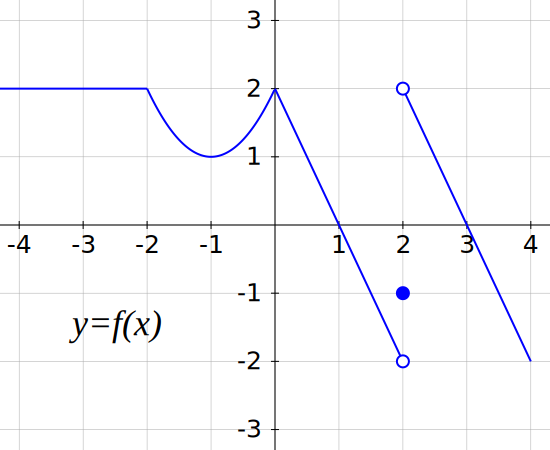
\includegraphics[scale=.4]{G1}

		\column{.33\textwidth}
		Find the value of
		\begin{enumerate}
			\item $\displaystyle \lim_{x \to 2}f(x)$

			\item $\displaystyle \lim_{x \to 0}f(f(x))$
			% \pause

			\item $\displaystyle \lim_{x \to 2}\left[ f(x) \right]^{2}$

			\item $\displaystyle \lim_{x \to 0}f(2 \cos x)$
		\end{enumerate}
	\end{columns}
\end{frame}

\begin{frame}[t]
	\frametitle{Floor}

	Given a real number $x$, we defined the \emph{floor of $x$}, denoted by $\lfloor
	x \rfloor$, as the largest integer smaller than or equal to $x$. For example:
	\[
		\lfloor \pi \rfloor= 3, \quad \quad \lfloor 7 \rfloor=7, \quad \quad \lfloor
		-0.5 \rfloor=-1.
	\]
	Sketch the graph of $\displaystyle y = \lfloor x \rfloor$. Then compute:
	\begin{multicols}{2}
		\begin{enumerate}
			\item $\displaystyle \lim_{x \to 0^+}\lfloor x \rfloor$

			\item $\displaystyle \lim_{x \to 0^-}\lfloor x \rfloor$

			\item $\displaystyle \lim_{x \to 0}\; \lfloor x \rfloor$

			\item $\displaystyle \lim_{x \to 0}\; \lfloor x^{2} \rfloor$
		\end{enumerate}
	\end{multicols}
\end{frame}

\begin{frame}
	\frametitle{More limits from a graph}

	\begin{columns}[c]
		\column{.65\textwidth}

		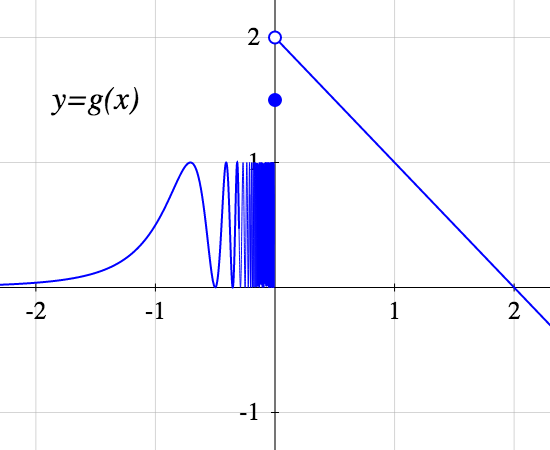
\includegraphics[scale=.4]{G2}

		\column{.33\textwidth}
		Find the value of
		\begin{enumerate}
			\item $\displaystyle \lim_{x \to 0^+}g(x)$

			\item $\displaystyle \lim_{x \to 0^+}\; \lfloor g(x) \rfloor$

			\item $\displaystyle \lim_{x \to 0^+}g(\lfloor x \rfloor)$

			\item $\displaystyle \lim_{x \to 0^-}g(x)$

			\item $\displaystyle \lim_{x \to 0^-}\; \lfloor g(x) \rfloor$

			\item $\displaystyle \lim_{x \to 0^-}\; \lfloor \frac{g(x)}{2}\rfloor$

			\item $\displaystyle \lim_{x \to 0^-}g(\lfloor x \rfloor)$
		\end{enumerate}
	\end{columns}
\end{frame}

\begin{frame}
	\frametitle{Limit at a point}

	If a function $f$ is not defined at $x=a$, then
	\begin{enumerate}
		\item $\displaystyle{\lim_{x\rightarrow a} f(x)}$ cannot exist

		\item $\displaystyle{\lim_{x\rightarrow a} f(x)}$ could be $0$

		\item $\displaystyle{\lim_{x\rightarrow a} f(x)}$ must approach $\infty$

		\item none of the above.
	\end{enumerate}
\end{frame}

\begin{frame}
	\frametitle{Evaluating Limits}

	\begin{itemize}
		\item You're trying to guess $\displaystyle{\lim_{x \rightarrow 0} f(x)}$.

		\item You plug in $x=0.1, 0.01, 0.001, \dots$ and get $f(x)=0$ for all these
			values.

		\item In fact, you're told that for all $n=1, 2, \dots$, $\displaystyle{f\left(\frac{1}{10^{n}}\right)}
			=0$. \\

		\item Can you conclude that $\displaystyle \lim_{x \rightarrow 0}f(x)=0$?
	\end{itemize}
\end{frame}

\begin{frame}
	\frametitle{Exponential limits}

	Compute:
	\[
		\lim_{t \to 0^+}e^{1/t}, \quad \quad \lim_{t \to 0^-}e^{1/t}.
	\]

	Suggestion: Sketch the graph of $\displaystyle y=e^{x}$ first.
\end{frame}

\begin{frame}[t]
	\frametitle{Rational limits}

	Consider the function
	\[
		h(x) = \frac{(x-1)(2+x)}{x^{2}(x-1)(2-x)}.
	\]
	\begin{itemize}
		\item Find all real values $a$ for which $h(a)$ is undefined. \\

		\item For each such value of $a$, compute
			$\displaystyle \lim_{x \to a^+}h(x)$ and
			$\displaystyle \lim_{x \to a^-}h(x)$. \\

		\item Based on your answer, and nothing else, try to sketch the graph of $h$.
	\end{itemize}
\end{frame}

\begin{frame}[t]
	\frametitle{$\delta$ from a graph}
	\fontsize{11}{11}\selectfont
	\begin{center}
		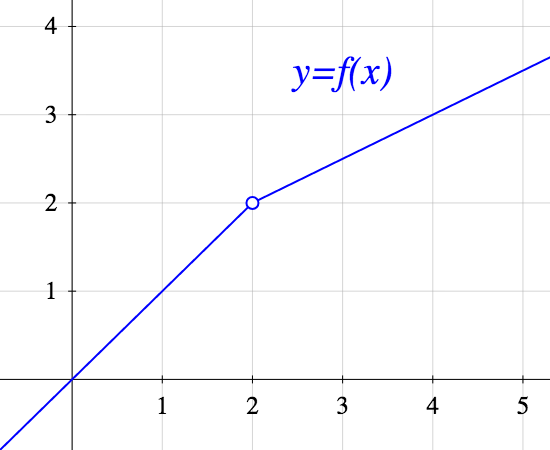
\includegraphics[scale=.3]{G3}
	\end{center}
	\begin{enumerate}
		\item Find one value of $\delta>0$ s.t. \hfill
			$\displaystyle 0 < |x-2| < \delta \implies |f(x) - 2| < 0.5$

		\item Find \emph{all} values of $\delta>0$ s.t. \hfill $\displaystyle 0 < |x-
			2| < \delta \implies |f(x) - 2| < 0.5$
	\end{enumerate}
\end{frame}

\begin{frame}
	\frametitle{Warm-up}

	Write down the formal definition of
	\[
		\lim_{x \to a}f(x) = L.
	\]
\end{frame}

\begin{frame}
	\frametitle{Side limits}

	\begin{block}{Recall}
		Let $L, a \in \mathbb{R}$. \\ Let $f$ be a function defined at least on an
		interval around $a$, except possibly at $a$. \\
		\[
			\lim_{x \to a}f(x) = L
		\]
		means
		\[
			\forall \varepsilon >0, \exists \delta >0 \text{ s.t. }\quad 0<|x-a|<\delta
			\implies |f(x)-L| < \varepsilon.
		\]
	\end{block}

	\vfill

	Write, instead, the formal definition of
	\[
		\lim_{x \to a^+}f(x) = L, \quad \text{ and }\quad \lim_{x \to a^-}f(x) = L.
	\]
\end{frame}

\begin{frame}
	\frametitle{Infinite limits}

	\begin{block}{Definition}
		Let $a \in \mathbb{R}$. \\ Let $f$ be a function defined at least on an
		interval around $a$, except possibly at $a$. \\ Write a formal definition
		for
		\[
			\lim_{x \to a}f(x) = \infty.
		\]
	\end{block}
\end{frame}

\begin{frame}[t]
	\frametitle{Infinite limits - 2}

	Which one(s) is the definition of $\displaystyle \lim_{x \to a}f(x) = \infty$ ?
	\vfill
	\begin{enumerate}
		\item $\displaystyle \forall M \in \mathbb{R}, \, \exists \delta > 0 \; \text{
			s.t. }0 < |x-a|<\delta \; \implies \; f(x) > M$
			\vfill

		\item $\displaystyle \forall M \in \mathbb{Z}, \, \exists \delta > 0 \; \text{
			s.t. }0 < |x-a|<\delta \; \implies \; f(x) > M$
			\vfill

		\item $\displaystyle \forall M > 0, \, \exists \delta > 0 \; \text{ s.t. }0 <
			|x-a|<\delta \; \implies \; f(x) > M$
			\vfill

		\item $\displaystyle \forall M > 5, \, \exists \delta > 0 \; \text{ s.t. }0 <
			|x-a|<\delta \; \implies \; f(x) > M$
			\vfill
		%	\item \DS{\forall M \in \R, \, \exists \delta > 0 \; \mbox{ s.t. } |x-a|<\delta \; \implies \; f(x) \geq M}

		%	\vfill
	\end{enumerate}
\end{frame}

\begin{frame}[t]
	\frametitle{Related implications}

	Let $a \in \mathbb{R}$. Let $f$ be a function. Assume we know
	\[
		0 < |x-a| < 0.1 \quad \implies \quad f(x) > 100
	\]
	\vspace{-.5cm}
	\begin{enumerate}
		\item Which values of $M \in \mathbb{R}$ satisfy ... ?
			\[
				0 < |x-a| < 0.1 \quad \implies \quad f(x) > M
				% \pause
			\]
			\vspace{-.5cm}

		\item Which values of $\delta>0$ satisfy ... ?
			\[
				0 < |x-a| < \delta \quad \implies \quad f(x) > 100
			\]
	\end{enumerate}
\end{frame}

\begin{frame}
	\frametitle{Strict or non-strict inequality?}

	Let $f$ be a function with domain $\mathbb{R}$. One of these statements implies
	the other. Which one?

	\begin{enumerate}
		\item $\displaystyle \forall M \in \mathbb{R}, \, \exists N \in \mathbb{R}\text{
			s.t. }x>N \implies f(x) > M$

		\item $\displaystyle \forall M \in \mathbb{R}, \, \exists N \in \mathbb{R}\text{
			s.t. }x>N \implies f(x) \geq M$
	\end{enumerate}
\end{frame}

\begin{frame}
	\frametitle{Negation of conditionals}

	Write the negation of these statements:
	\begin{enumerate}
		\item If Justin Trudeau has a brother, then he also has a sister.

		\item If a student in this class has a brother, then they also have a sister.
	\end{enumerate}
\end{frame}

\begin{frame}
	\frametitle{More negation}

	Let $f$ be a function with domain $\mathbb{R}$. Write the negation of the statement:
	\begin{equation*}
		\text{IF }\; 2<x<4, \quad \text{ THEN }\; 1<f(x)<3.
	\end{equation*}
\end{frame}

\begin{frame}
	\frametitle{Existence}

	Write down the formal definition of the following statements:

	\vfill
	\begin{enumerate}
		\item $\displaystyle \lim_{x \to a}f(x) = L$
			\vfill

		\item $\displaystyle \lim_{x \to a}f(x)$ exists

			\vfill

		\item $\displaystyle \lim_{x \to a}f(x)$ does not exist
	\end{enumerate}

	\vfill
\end{frame}

\begin{frame}[t]
	\frametitle{Preparation: choosing deltas}

	\begin{enumerate}
		\item Find one value of $\delta >0$ such that
			\[
				|x-3|< \delta \implies |5x-15|<1.
			\]

		\item Find \emph{all} values of $\delta >0$ such that
			\[
				|x-3|< \delta \implies |5x-15|<1.
			\]

		\item Find \emph{all} values of $\delta >0$ such that
			\[
				|x-3|< \delta \implies |5x-15|<0.1.
			\]

		\item Let us fix $\varepsilon >0$. Find \emph{all} values of $\delta >0$ such
			that
			\[
				|x-3|< \delta \implies |5x-15|<\varepsilon.
			\]
	\end{enumerate}
\end{frame}

\begin{frame}
	\frametitle{What is wrong with this ``proof"?}
	\fontsize{13}{13}\selectfont
	\vspace{-2mm}
	\begin{block}{}%$\varepsilon-\delta$ Proofs}
		Prove that
		\[
			\lim_{x\to 3}(5x+1) = 16
		\]
	\end{block}

	\begin{block}{``Proof:"}
		Let $\varepsilon>0$.

		WTS $\forall \varepsilon>0$, $\exists\delta>0$ s.t.
		\[
			0<|x-3|<\delta \implies |(5x+1) - (16)|<\varepsilon
		\]
		\vspace{-3mm}
		\begin{align*}
			|(5x+1) - (16)|<\varepsilon & \iff |5x+15|<\varepsilon                                     \\
			                            & \iff 5|x+3|<\varepsilon \implies\delta=\frac{\varepsilon}{3}
		\end{align*}
		\hfill $\square$
	\end{block}
\end{frame}

\begin{frame}[t]
	\frametitle{Your first $\varepsilon-\delta$ proof}

	\begin{block}{Goal}
		We want to prove that
		\begin{equation}
			\label{eq:uno}\lim_{x \to 3}\left( 5x + 1 \right) = 16
		\end{equation}
		directly from the definition.
	\end{block}
	\vfill
	\begin{enumerate}
		% \pause

		\item Write down the formal definition of the statement \eqref{eq:uno}.
		% \pause

		\item Write down what the structure of the formal proof should be, without
			filling the details.
		% \pause

		\item Write down a complete formal proof.
	\end{enumerate}
	\vfill
\end{frame}

\begin{frame}
	\frametitle{A harder proof}

	\begin{block}{Goal}
		We want to prove that
		\begin{equation}
			\label{eq:dos}\lim_{x \to 0}\left( x^{3}+ x^{2}\right) = 0
		\end{equation}
		directly from the definition.
	\end{block}
	\vfill
	\begin{enumerate}
		% \pause

		\item Write down the formal definition of the statement \eqref{eq:dos}.
		% \pause

		\item Write down what the structure of the formal proof should be, without
			filling the details.
		% \pause

		\item Rough work: What is $\delta?$
		% \pause

		\item Write down a complete formal proof.
	\end{enumerate}
	\vfill
\end{frame}

\begin{frame}[t]
	\frametitle{Is this proof correct?}

	{\bfseries Claim:}
	\[
		\forall \varepsilon >0, \exists \delta>0 \text{ s.t. }\quad 0<|x|<\delta \; \implies
		\; |x^{3}+x^{2}| < \varepsilon.
	\]
	\vfill
	\begin{block}{Proof:}
		\begin{itemize}
			\item Let $\varepsilon >0$.

			\item Take $\displaystyle \delta = \sqrt{\frac{\varepsilon}{|x+1|}}$.

			\item Let $x \in \mathbb{R}$. Assume $0 < |x| < \delta$. Then
				\[
					|x^{3}+x^{2}| = x^{2}| x + 1| < \delta^{2}|x+1| = \frac{\varepsilon}{|x+1|}
					|x+1| = \varepsilon.
				\]

			\item I have proven that $\displaystyle |x^{3}+x^{2}| < \varepsilon$.
				\hfill \qed
		\end{itemize}
	\end{block}

	\vfill
\end{frame}

\begin{frame}[t]
	\frametitle{Choosing deltas again}

	Let us fix numbers $A, \varepsilon >0$. Find:

	\vfill

	\begin{enumerate}
		\item a value of $\delta >0$ \; s.t. \hfill
			$\displaystyle |x|< \delta \implies |Ax^{2}|<\varepsilon$
			% \pause
			\vfill

		\item \emph{all} values of $\delta >0$ \; s.t. \hfill $\displaystyle |x|< \delta
			\implies |Ax^{2}|<\varepsilon$
			% \pause
			\vfill

		\item a value of $\delta >0$ \; s.t. \hfill
			$\displaystyle |x|< \delta \implies |x+1| < 10$
			% \pause
			\vfill

		\item \emph{all} values of $\delta >0$ \; s.t. \hfill $\displaystyle |x|< \delta
			\implies |x+1| < 10$
			% \pause
			\vfill

		\item a value of $\delta >0$ \; s.t. \hfill
			$\displaystyle |x|< \delta \implies \left\{
			\begin{array}{c}
				|Ax^2|<\varepsilon \\
				|x+1| < 10
			\end{array}
			\right.$
			% \pause
			\vfill

		\item a value of $\delta >0$ \; s.t. \hfill
			$\displaystyle |x| < \delta \implies |(x+1)x^{2}| < \varepsilon$
			\vfill
	\end{enumerate}
\end{frame}

\begin{frame}[t]
	\frametitle{Indeterminate form}

	Let $a \in \mathbb{R}$. Let $f$ and $g$ be positive functions defined near $a$,
	except maybe at $a$.

	\vfill

	Assume $\displaystyle \lim_{x \to a}f(x) = \lim_{x \to a}g(x) = 0$.

	\vfill

	What can we conclude about \quad
	$\displaystyle \lim_{x \to a}\frac{f(x)}{g(x)}$ ?

	\vfill

	\begin{multicols}{2}
		\begin{enumerate}
			\item The limit is $1$.

			\item The limit is $0$.

			\item The limit is $\infty$.

			\item The limit does not exist.

			\item We do not have enough information to decide.
		\end{enumerate}
	\end{multicols}
\end{frame}

\begin{frame}
	\frametitle{A theorem about limits}
	\fontsize{13}{13}\selectfont
	\begin{block}{}
		Let $f$ be a function with domain $\mathbb{R}$ such that
		\[
			\lim_{x\to 0}f(x) = 3
		\]
		Prove that
		\[
			\lim_{x\to 0}\left[ 5 f(2x) \right] =15
		\]
		directly from the definition of limit. Do not use any of the limit laws.
	\end{block}
	\begin{enumerate}
		% \pause

		\item Write down the formal definition of the statement you want to prove.
		% \pause

		\item Write down what the structure of the formal proof should be, without
			filling the details.
		% \pause

		\item Rough work.
		% \pause

		\item Write down a complete proof.
	\end{enumerate}
\end{frame}

\begin{frame}[t]
	\frametitle{Proof feedback}

	\begin{enumerate}
		\item Is the structure of the proof correct? \\ (First fix $\varepsilon$,
			then choose $\delta$, then ...)

		\item Did you say exactly what $\delta$ is?

		\item Is the proof self-contained? \\ (I do not need to read the rough work)

		\item Are all variables defined? In the right order?

		\item Do all steps follow logically from what comes before? \\ Do you start
			from what you know and prove what you have to prove? \\

		\item Are you proving your conclusion or assuming it?
	\end{enumerate}
\end{frame}

\begin{frame}[t]
	\frametitle{A new squeeze}
	\fontsize{13}{13}\selectfont This is the Squeeze Theorem, as you know it:

	\begin{block}{The (classical) Squeeze Theorem}
		Let $a, L \in \mathbb{R}$. \\ Let $f$, $g$, and $h$ be functions defined
		near $a$, except possibly at $a$.

		\vspace{.2cm}
		\begin{tabular}{cl}
			IF             & $\bullet$ {For $x$ close to $a$ but not $a$,} \; $\displaystyle h(x) \leq g(x) \leq f(x)$              \\
			\vspace{-0.2cm} \\
			               & $\bullet$ $\displaystyle \lim_{x \to a}f(x) = L$ \quad and \quad$\displaystyle \lim_{x \to a}h(x) = L$ \\
			\vspace{-.1cm}  \\
			THEN           & $\bullet$ $\displaystyle \lim_{x \to a}g(x) = L$
		\end{tabular}
	\end{block}

	% \pause
	Come up with a new version of the theorem about limits being infinity. (The
	conclusion should be $\displaystyle \lim_{x \to a}g(x) = \infty$.)

	\emph{Hint:} Draw a picture for the classical Squeeze Theorem. Then draw a picture
	for the new theorem.
\end{frame}

\begin{frame}[t]
	\frametitle{A new squeeze}
	\fontsize{13}{13}\selectfont
	\begin{block}{The (new) Squeeze Theorem}
		Let $a \in \mathbb{R}$. \\ Let $g$ and $h$ be functions defined near $a$, except
		possibly at $a$.

		\vspace{.2cm}
		\begin{tabular}{cl}
			IF            & $\bullet$ {For $x$ close to $a$ but not $a$,} \; $\displaystyle %\exists p >0, \mbox{ s.t. } 0 < |x-a| < p \; \implies \; 
h(x) \leq g(x)$ \\
			\vspace{-.2cm} \\
			              & $\bullet$ $\displaystyle \lim_{x \to a}h(x) = \infty$                                                                                      \\
			\vspace{-.1cm} \\
			THEN          & $\bullet$ $\displaystyle \lim_{x \to a}g(x) = \infty$
		\end{tabular}
	\end{block}

	\begin{enumerate}
		% \pause

		\item Replace the first hypothesis with a more precise mathematical statement.
		% \pause

		\item Write down the definition of what you want to prove.
		% \pause

		\item Write down the structure of the formal proof.
		% \pause

		\item Rough work
		% \pause

		\item Write down a complete, formal proof.
	\end{enumerate}
\end{frame}

\begin{frame}
	\frametitle{True or False?}

	\vfill

	Is this theorem true?

	\vfill

	\begin{block}{Claim}
		Let $a \in \mathbb{R}$. \\ Let $f$ and $g$ be functions defined near $a$. \\
		\begin{itemize}
			\item IF $\displaystyle \lim_{x \to a}f(x) = 0$,

			\item THEN $\displaystyle \lim_{x \to a}\left[ f(x) g(x) \right] = 0$.
		\end{itemize}
	\end{block}

	\vfill
\end{frame}

\begin{frame}[t]
	\frametitle{A new theorem about products}
	\fontsize{13}{13}\selectfont
	\begin{block}{Theorem}
		Let $a \in \mathbb{R}$. Let $f$ and $g$ be functions with domain
		$\mathbb{R}$, except possibly $a$. Assume
		\begin{itemize}
			\item $\displaystyle \lim_{x \to a}f(x) = 0$, and

			\item $g$ is bounded. This means that
				\[
					\exists M >0 \text{ s.t. }\forall x \neq a, |g(x)| \leq M.
				\]
		\end{itemize}
		THEN $\displaystyle \lim_{x \to a}\left[ f(x) g(x) \right] = 0$
	\end{block}

	\vfill
	\begin{enumerate}
		% \pause

		\item Write down the formal definition of what you want to prove.
		% \pause

		\item Write down what the structure of the formal proof.
		% \pause

		\item Rough work.
		% \pause

		\item Write down a complete formal proof.
	\end{enumerate}
	\vfill
\end{frame}

\begin{frame}[t]
	\frametitle{Critique this ``proof" -- \#1}
	\fontsize{13}{13}\selectfont
	\begin{itemize}
		\item WTS $\displaystyle \lim_{x \to a}\left[ f(x) g(x) \right] = 0$:

			\hfill $\displaystyle \forall \varepsilon>0, \exists \delta>0$ \; s.t. \;
			$\displaystyle 0<|x-a|<\delta \implies{\color{blue} |f(x) g(x)| < \varepsilon}$.
			\vfill

		\item We know $\displaystyle \lim_{x \to a}f(x) = 0$

			\hfill $\displaystyle \forall \varepsilon_{1}>0, \exists \delta_{1}>0$ \;
			s.t. \; $\displaystyle 0<|x-a|<\delta_{1}\implies{\color{blue} |f(x)| <\varepsilon_1}$.
			\vfill

		\item We know \hfill $\displaystyle \exists M>0$ \; s.t. \;
			$\displaystyle \forall x \neq 0, \; \;{\color{blue} |g(x)| \leq M}$.
			\vfill

		\item $\displaystyle |f(x)g(x)| = |f(x)||g(x)| < \varepsilon_{1}M$
			\vfill

		\item $\displaystyle \varepsilon = \varepsilon_{1}M \implies \varepsilon_{1}=
			\frac{\varepsilon}{M}$
			\vfill

		\item Take $\displaystyle \delta = \delta_{1}$
			\vfill
	\end{itemize}
\end{frame}

\begin{frame}[t]
	\frametitle{Critique this ``proof" -- \#2}
	\fontsize{13}{13}\selectfont
	\begin{itemize}
		\item WTS $\displaystyle \lim_{x \to a}\left[f(x) g(x) \right] =0$. By
			definition, WTS:

			\hfill $\displaystyle \forall \varepsilon>0, \exists \delta>0$ s.t.
			$\displaystyle 0<|x-a|<\delta \implies |f(x) g(x)|<\varepsilon$
			\vfill

		\item Let $\varepsilon >0$.
			\vfill

		\item Use the value $\displaystyle \frac{\varepsilon}{M}$ as ``epsilon" in
			the definition of $\displaystyle \lim_{x \to a}f(x) = 0$

			\hfill $\displaystyle \exists \delta_{1}\in \mathbb{R}$ s.t.
			$\displaystyle 0<|x-a|<\delta_{1}\implies |f(x)| < \frac{\varepsilon}{M}$.
			\vfill

		\item Take $\displaystyle \delta = \delta_{1}$.
			\vfill

		\item Let $\displaystyle x \in \mathbb{R}$. Assume
			$\displaystyle 0 < |x-a| <\delta$
			\vfill

		\item Since $\displaystyle \exists M>0$ s.t.
			$\displaystyle \forall x \neq 0, |g(x)| \leq M$ \\ \hfill
			$\displaystyle |f(x) g(x)| < \frac{\varepsilon}{M}\cdot M = \varepsilon$.
			\vfill
	\end{itemize}
\end{frame}

\begin{frame}[t]
	\frametitle{Critique this ``proof" -- \#3}
	\fontsize{13}{13}\selectfont
	\begin{itemize}
		\item Since $g$ is bounded, $\displaystyle \exists M >0$ \; s.t. \; \;$\displaystyle
			\forall x \neq 0, \; |g(x)| \leq M$
			\vfill

		\item Since $\displaystyle \lim_{x \to a}f(x)=0$, there exists
			$\displaystyle \delta_{1}>0$ s.t.

			if $\displaystyle 0<|x-a|<\delta_{1}$, \quad then \; $\displaystyle |f(x)-0
			| = |f(x)| <\varepsilon_{1}= \frac{\varepsilon}{M}$.
			\vfill

		\item \
			\vspace{-1cm}
			\[
				|f(x)g(x)| = |f(x)| \cdot |g(x)| \leq |f(x)| \cdot M < \varepsilon_{1}\cdot
				M = \frac{\varepsilon}{M}\cdot M = \varepsilon
			\]

		\item In summary, by setting $\displaystyle \delta = \min\{\delta_{1}\}$, we
			find that

			if $\displaystyle 0<|x-a|<\delta$, \quad then \; $\displaystyle |f(x) \cdot
			g(x)| < \varepsilon$.
			\vfill
	\end{itemize}
\end{frame}

\begin{frame}
	\frametitle{Limits involving $\displaystyle \sin(1/x)$ Part I}

	\begin{block}{ The reason that $\displaystyle{\lim_{x\rightarrow 0}\sin (1/x)}$
	does not exist is:}
		\begin{enumerate}
			\item because the function values oscillate around $0$

			\item because $1/0$ is undefined

			\item because no matter how close $x$ gets to $0$, there are $x$'s near
				$0$ for which $\sin(1/x) =1$, and some for which $\sin (1/x)=-1$

			\item all of the above
		\end{enumerate}
	\end{block}
\end{frame}

\begin{frame}
	\frametitle{Limits involving $\displaystyle \sin(1/x)$ Part II}

	\begin{block}{The limit $\displaystyle{\lim_{x\rightarrow 0}x^2\sin (1/x)}$ }
		\begin{enumerate}
			\item does not exist because the function values oscillate around $0$

			\item does not exist because $1/0$ is undefined

			\item does not exist because no matter how close $x$ gets to $0$, there
				are $x$'s near $0$ for which $\sin(1/x) =1$, and some for which $\sin (1/
				x)=-1$

			\item equals 0

			\item equals 1
		\end{enumerate}
	\end{block}
\end{frame}

\begin{frame}
	\frametitle{Absolute value and the Squeeze Theorem}

	Use the Squeeze Theorem to prove:
	\begin{theorem}
		IF $\displaystyle \lim_{x\to a}|f(x)| = 0$, THEN
		$\displaystyle \lim_{x\to a}f(x)=0$.\\
	\end{theorem}

	\emph{Hint:} Recall that $-|c| \leq c \leq |c|$ for every $c \in \mathbb{R}$.
\end{frame}

\begin{frame}[t]
	\frametitle{Undefined function}
	\fontsize{13}{13}\selectfont Let $a \in \mathbb{R}$ and let $f$ be a function.
	Assume $f(a)$ is undefined.

	\vfill

	\begin{block}{What can we conclude?}
		\begin{enumerate}
			\item $\displaystyle \lim_{x \to a}f(x)$ exist

			\item $\displaystyle \lim_{x \to a}f(x)$ doesn't exist.

			\item No conclusion. $\displaystyle \lim_{x \to a}f(x)$ may or may not
				exist.
		\end{enumerate}
	\end{block}

	\vfill

	\begin{block}{What else can we conclude?}
		\begin{enumerate}
			\addtocounter{enumi}{3}

			\item $f$ is continuous at $a$.

			\item $f$ is not continuous at $a$.

			\item No conclusion. $f$ may or may not be continuous at $a$.
		\end{enumerate}
	\end{block}

	\vfill
\end{frame}

\begin{frame}
	\frametitle{A new function}

	\begin{itemize}
		\item Let $x, y \in \mathbb{R}$. What does the following expression
			calculate? Prove it.
			\[
				f(x,y) = \frac{x + y + |x - y|}{2}
			\]
			\emph{Suggestion:} If you don't know how to start, try some sample values
			of $x$ and $y$.
			\vfill
		% \pause

		\item Write a similar expression to compute $\displaystyle \min \{ x, y \}$.
	\end{itemize}
	\vfill
\end{frame}

\begin{frame}
	\frametitle{More continuous functions}

	We want to prove the following theorem
	\begin{block}{Theorem}
		IF $f$ and $g$ are continuous functions \\ THEN $h(x) = \max \{ f(x), g(x) \}$
		is also a continuous function.
	\end{block}

	You are allowed to use all results that we already know. What is the fastest
	way to prove this?

	\vfill

	\emph{Hint:} There is a way to prove this quickly without writing any epsilons.

	\vfill
\end{frame}

\begin{frame}
	\frametitle{True or False? -- Discontinuities}

	\begin{enumerate}
		\item IF $f$ and $g$ have removable discontinuities at $a$

			THEN $f+g$ has a removable discontinuity at $a$

		\item IF $f$ and $g$ have non-removable discontinuities at $a$

			THEN $f+g$ has a non-removable discontinuity at $a$
	\end{enumerate}
\end{frame}

\begin{frame}
	\frametitle{Which one is the correct claim?}

	\begin{block}{Claim 1?}
		(Assuming these limits exist)
		\[
			\lim_{x \to a}g(f(x)) \; = \; g \left( \lim_{x \to a}f(x) \right)
		\]
	\end{block}

	\vfill

	\begin{block}{Claim 2?}
		\begin{tabular}{lll}
			IF   & {\color{blue} (A)} $\displaystyle \lim_{x \to a}f(x) = L$, \quad and & {\color{blue} (B)} $\displaystyle \lim_{t \to L}g(t) = M \ $ \\
			THEN & {\color{blue} (C)} $\displaystyle \lim_{x \to a}g(f(x)) = M \;$
		\end{tabular}
	\end{block}
\end{frame}

\begin{frame}
	\frametitle{A difficult example}

	Construct a pair of functions $f$ and $g$ such that
	\begin{align*}
		\lim_{x \to 0}f(x) \;    & \; = \; 1  \\
		\lim_{t \to 1}g(t) \;    & \; = \; 2  \\
		\lim_{x \to 0}g(f(x)) \; & \; = \; 42
	\end{align*}
\end{frame}

\begin{frame}
	\frametitle{Transforming limits}

	The only thing we know about the function $g$ is that
	\[
		\lim_{x \to 0}\frac{g(x)}{x^{2}}= 2.
	\]
	Use it to compute the following limits:

	\begin{multicols}{2}
		\begin{enumerate}
			\item $\displaystyle \lim_{x \to 0}\frac{g(x)}{x}$

			\item $\displaystyle \lim_{x \to 0}\frac{g(x)}{x^{4}}$

			\item $\displaystyle \lim_{x \to 0}\frac{g(3x)}{x^{2}}$
		\end{enumerate}
	\end{multicols}
\end{frame}

\begin{frame}
	\frametitle{Limits at infinity}

	Compute:

	\begin{enumerate}
		\begin{multicols}{2}
			\item $\displaystyle \lim_{x \to \infty}\left(x^{7}-2x^{5}+11\right)$ \item
			$\displaystyle \lim_{x \to \infty}\left(x^{2}- \sqrt{x^{5}+1}\right)$ \item
			$\displaystyle \lim_{x \to \infty}\frac{x^{2}+11}{x+1}$ \item $\displaystyle
			\lim_{x \to \infty}\frac{x^{2}+2x+3}{3x^{2}+4x+5}$

			\item
			$\displaystyle \lim_{x \to \infty}\frac{x^{3}+ \sqrt{2x^6+1}}{2x^{3}+ \sqrt{x^5+1}}$
		\end{multicols}
	\end{enumerate}
\end{frame}

\begin{frame}
	\frametitle{Trig computations}

	Using that $\displaystyle \lim_{x \to 0}\frac{\sin x}{x}= 1$, compute the following
	limits:

	\begin{enumerate}
		\begin{multicols}{2}
			\item $\displaystyle \lim_{x \to 2}\frac{\sin x}{x}$ \item $\displaystyle \lim
			_{x \to 0}\frac{\sin (5x)}{x}$ \item $\displaystyle \lim_{x \to 0}\frac{\tan^{2}(2x^{2})}{
			x^{4}}$ \item $\displaystyle \lim_{x \to 0}\frac{\sin e^{x}}{e^{x}}$ \item
			$\displaystyle \lim_{x \to 0}\frac{1 - \cos x}{x}$ \item $\displaystyle \lim
			_{x \to 0}\frac{\tan^{10}(2x^{20})}{\sin^{200}(3x)}$
		\end{multicols}
		% \pause

		\item \
			\vspace{-.6cm}

			{\fontsize{13}{13}\selectfont $\displaystyle \lim_{x \to 0}\left[ (\sin x) \; (\cos (2x)) \; (\tan (3x)) \; (\sec (4x) ) \; (\csc (5x)) \; (\cot (6x)) \right]$ }
	\end{enumerate}
\end{frame}

\begin{frame}
	\frametitle{Plus or minus infinity?}

	Compute:
	\begin{enumerate}
		\begin{multicols}{2}
			\item $\displaystyle \lim_{x \to -3^+}\; \frac{x^{2}-9}{3-2x-x^{2}}$

			\item $\displaystyle \lim_{x \to 1^+}\; \frac{x^{2}-9}{3-2x-x^{2}}$
		\end{multicols}
	\end{enumerate}
\end{frame}

\begin{frame}
	\frametitle{A harder limit}

	Calculate

	\[
		\lim_{x \to 2}\frac{\left[\sqrt{2+x} -2\right] \left[ \sqrt{3+x} - 3 \right]}{\sqrt{x-1}
		- 1}
	\]
\end{frame}

\begin{frame}
	\fontsize{13}{13}\selectfont
	\frametitle{Which solution is right?}
	Compute
	$\displaystyle L = \lim_{x \to -\infty}\left[ x - \sqrt{x^{2}+x}\right]$.

	\begin{itemize}
		\item {\bfseries Solution 1} {\fontsize{11}{11}\selectfont \begin{align*}L =&\lim_{x\to -\infty}\frac{\left[ x - \sqrt{x^{2}+x} \right] \; \left[ x + \sqrt{x^{2}+x} \right]}{\left[ x + \sqrt{x^{2}+x} \right]}= \lim_{x \to -\infty}\frac{x^{2}-(x^{2}+x)}{\left[ x + \sqrt{x^{2}+x} \right]}\\ =&\lim_{x \to -\infty}\frac{-x}{x \left[ 1 + \sqrt{1 + \frac{1}{x}} \right]}= \lim_{x \to -\infty}\frac{-1}{ \left[ 1 + \sqrt{1 + \frac{1}{x}} \right]}= \frac{-1}{2}\end{align*} }

		\item {\bfseries Solution 2}
			\[
				L = \lim_{x \to -\infty}\left[{\color{red} x }-{\color{blue} \sqrt{x^{2}+x} }
				\right] ={\color{red}(-\infty)}-{\color{blue}\infty}= - \infty
			\]
	\end{itemize}
\end{frame}

\begin{frame}
	\frametitle{Can we conclude this?}

	\begin{itemize}
		\item Consider the function $\displaystyle (x)=\frac{4}{x}$.
			\vfill

		\item We have \quad $f(-1)=-4<0$ \quad and \quad $f(1)=4>0$.
			\vfill

		\item Use IVT.

			Can we conclude $f(c)=0$ for some $c\in(-1,1)$?
	\end{itemize}
	\vfill
	\vfill
\end{frame}

\begin{frame}
	\frametitle{Existence of solutions}

	Prove that the equation
	\[
		x^{4}- 2x = 100
	\]
	has at least two solutions.
\end{frame}

\begin{frame}[t]
	\frametitle{Can this be proven? (Use IVT)}
	\fontsize{13}{13}\selectfont
	\begin{enumerate}
		\item Prove that there exists a time of the day when the hour hand and the minute
			hand of a clock form an angle of exactly 23 degrees.

			% \pause
			\vfill

		\item During a Raptors basketball game, at half time the Raptors have 52
			points. Prove that at some point they had exactly 26 points.

			% \pause
			\vfill

		\item Prove that at some point during Alfonso's life, his height in
			centimetres was exactly equal to 10 times his weight in kilograms. Some data:
			\begin{itemize}
				\item His height at birth: 47 cm

				\item His weight at birth: 3.2 kg

				\item His height today: 172 cm
			\end{itemize}
			\vfill
	\end{enumerate}
\end{frame}

\begin{frame}
	\frametitle{Temperature}

	On June 09, 2016, the outside temperature in Toronto at 6 AM was $10^{\circ}$.
	At 4 PM, the temperature was $20^{\circ}$.

	\begin{enumerate}
		\item Must there have been a time between 6 AM and 4 PM when the temperature
			was $15^{\circ}$? Explain how you know. Which assumption about temperature
			allows you to reach your conclusion?

		\item Must there have been a time between 6 AM and 4 PM when the temperature
			was $22^{\circ}$? Explain how you know.

		\item Could there have been a time between 6 AM and 4 PM when the temperature
			was $22^{\circ}$? Explain how you know.
	\end{enumerate}
\end{frame}

\begin{frame}
	\frametitle{Extrema}

	In each of the following cases, does the function $f$ have a maximum and a minimum
	on the interval $I$?

	\begin{enumerate}
		\item $\displaystyle f(x) = x^{2}$, \quad $\displaystyle I = (-1,1)$.

		\item $\displaystyle f(x) = \frac{(e^{x}+ 2) \sin x}{x}- \cos x + 3$, \quad
			$\displaystyle I = [2,6]$

		\item $\displaystyle f(x) = \frac{(e^{x}+ 2) \sin x}{x}- \cos x + 3$, \quad
			$\displaystyle I = (0,5]$
	\end{enumerate}
\end{frame}

\begin{frame}
	\frametitle{Definition of maximum}

	Let $f$ be a function with domain $I$. \\ Which one (or ones) of the following
	is (or are) a definition of \quad ``$f$ has a maximum on $I$"?

	\begin{enumerate}
		\item $\displaystyle \forall x \in I$,
			$\displaystyle \exists C \in \mathbb{R}$ s.t. $\displaystyle f(x) \leq C$

		\item $\displaystyle \exists C \in I$ s.t. $\displaystyle \forall x \in I$, $\displaystyle
			f(x) \leq C$

		\item $\displaystyle \exists C \in \mathbb{R}$ s.t.
			$\displaystyle \forall x \in I$, $\displaystyle f(x) \leq C$

		\item $\displaystyle \exists C \in \mathbb{R}$ s.t.
			$\displaystyle \forall x \in I$, $\displaystyle f(x) < C$
	\end{enumerate}
\end{frame}

\begin{frame}
	\frametitle{More on the definition of maximum}

	Let $f$ be a function with domain $I$. \\ What does each of the following mean?

	\begin{enumerate}
		\item $\displaystyle \exists C \in \mathbb{R}$ s.t.
			$\displaystyle \forall x \in I$, $\displaystyle f(x) \leq C$

		\item $\displaystyle \exists C \in \mathbb{R}$ s.t.
			$\displaystyle \forall x \in I$, $\displaystyle f(x) < C$

		\item $\displaystyle \exists a \in I$ s.t. $\displaystyle \forall x \in I$, $\displaystyle
			f(x) \leq f(a)$

		\item $\displaystyle \exists a \in I$ s.t. $\displaystyle \forall x \in I$, $\displaystyle
			f(x) < f(a)$
	\end{enumerate}
\end{frame}

\begin{frame}[t]
	\frametitle{Tangent line to a line?}

	What is the equation of the line tangent to the graph of $y=x$ at the point
	with $x$--coordinate $7$?

	\begin{enumerate}
		\item $\displaystyle y=x+7$

		\item $\displaystyle y=x$

		\item $\displaystyle y=7$

		\item $\displaystyle x=7$

		\item There is no tangent line at that point.

		\item There is more than one tangent line at that point.
	\end{enumerate}
\end{frame}

\begin{frame}
	\frametitle{Prove these statements are false with counterexamples}

	Let $C$ be a curve. Let $P$ be a point in $C$.
	\vfill
	\begin{enumerate}
		\item The line tangent to $C$ at $P$ \\ intersects $C$ at only one point:
			$P$.
			\vfill

		\item If a line intersects $C$ only at $P$, \\ then that line must be the
			tangent line to $C$ at $P$.
			\vfill

		\item The tangent line to $C$ at $P$ intersects $C$ at $P$ \\ and ``does not
			cross'' $C$ at $P$. \\ (This means that, near $P$, it stays on one side of
			$C$.)
			\vfill

		\item If a line intersects $C$ at $P$ \\ and ``does not cross'' $C$ at $P$,
			\\ then it is the tangent line to $C$ at $P$.
			\vfill
	\end{enumerate}
\end{frame}

\begin{frame}[t]
	\frametitle{Tangent line from a graph}
	This is the graph of the function $f$. Write the equation of the line tangent
	to it at the point with $x$--coordinate $-2$.
	\begin{center}
		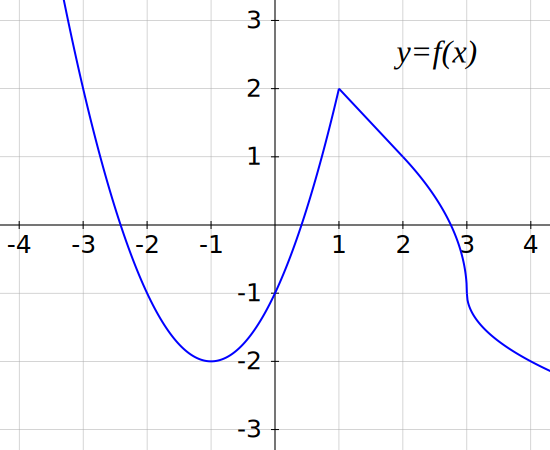
\includegraphics[scale=.4]{G4}
	\end{center}
\end{frame}

\begin{frame}[t]
	\frametitle{Derivative from a graph}
	This is the graph of the function $f$. \\ Sketch the graph of its derivative
	$f'$.
	\begin{center}
		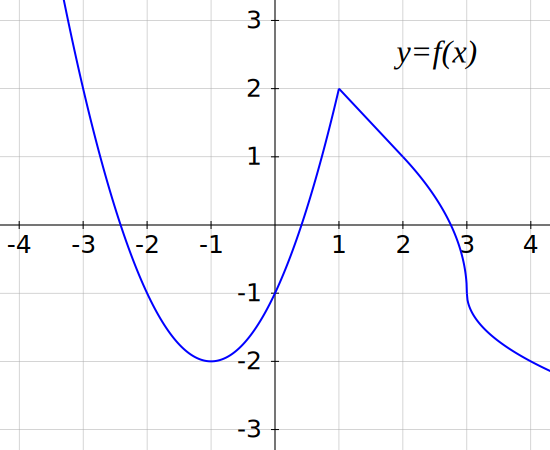
\includegraphics[scale=.4]{G4}
	\end{center}
\end{frame}

\begin{frame}[t]
	\frametitle{From the derivative to the function}

	\begin{enumerate}
		\item Sketch the graph of a continuous function with domain $\mathbb{R}$,
			whose derivative has the graph below.

		\item Sketch the graph of a non-continuous function whose derivative has the
			graph below.
	\end{enumerate}

	\begin{center}
		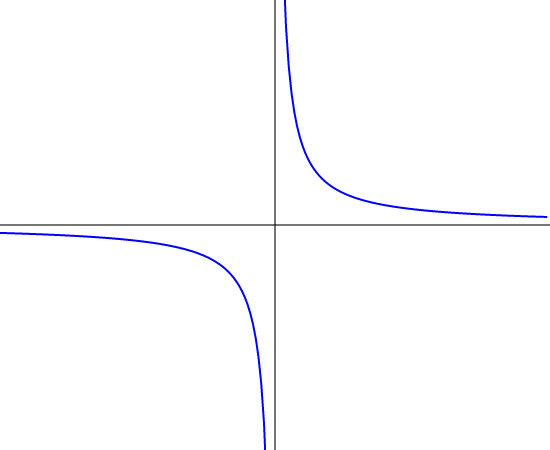
\includegraphics[scale=.3]{G5}
	\end{center}
\end{frame}

\begin{frame}
	\frametitle{Estimations - 1}

	Let $f$ be a continuous function with domain $\mathbb{R}$.

	\vfill

	\begin{enumerate}
		\item We know $f(4)=3$ and $f(4.2)=2.2$. \\ Based only on this, give your best
			estimate for $f(4.1)$.
			\vfill

		\item We know $f(4)=3$ and $f'(4)=0.6$. \\ Based only on this, give your best
			estimate for $f(4.1)$.
			\vfill

		\item We know $f(4)=3$ and $f(4.1) = 4$. \\ Based only on this, give your best
			estimate for $f'(4)$.
	\end{enumerate}

	\vfill
\end{frame}

\begin{frame}
	\frametitle{Estimations -- 2}

	Without using a calculator, estimate $\displaystyle \sqrt[20]{1.01}$ as well as
	you can.

	\emph{Hint:} You know the value of $\displaystyle f(x) = \sqrt[20]{x}$ and its
	derivative at one point very close to 1.01. Use the tangent line at that point
	as an approximation.
\end{frame}

\begin{frame}[t]
	\fontsize{13}{13}\selectfont
	\frametitle{Estimations -- 3}

	%The point of this question is to make them discover L'Hopital's Rule!

	\begin{enumerate}
		\item We know \quad $\displaystyle f(0) = 2, \quad f'(0) = 3, \quad g(0) = 7,
			\quad g'(0) = 5.$

			\vspace{.2cm}
			Compute \; $\displaystyle \lim_{x \to 0}\frac{f(x)}{g(x)}$.

			\vfill

		\item We know \quad $\displaystyle f(0) = 0, \quad f'(0) = 3, \quad g(0) = 0,
			\quad g'(0) = 5.$

			\vspace{.2cm}
			\begin{itemize}
				\item When $x$ is close to $0$, give estimates for $\displaystyle f(x)$
					and $\displaystyle g(x)$ using the tangent lines at $0$.

				\item Use those estimates to compute \; $\displaystyle \lim_{x \to 0}\frac{f(x)}{g(x)}$.
			\end{itemize}
	\end{enumerate}

	\vfill
\end{frame}

\begin{frame}[t]
	\frametitle{Derivatives from the definition}

	Let
	\[
		g(x) = \frac{2}{\sqrt{x}}
	\]

	Calculate $\displaystyle g'(4)$ directly from the definition of derivative as a
	limit.
\end{frame}

\begin{frame}
	\frametitle{Bella}

	The graph below describes Bella's distance from home one morning as she drives
	drive between her home and school.\\

	Describe a possible scenario for her travels that morning. \\ Then sketch the
	corresponding graph of his velocity.

	\begin{center}
		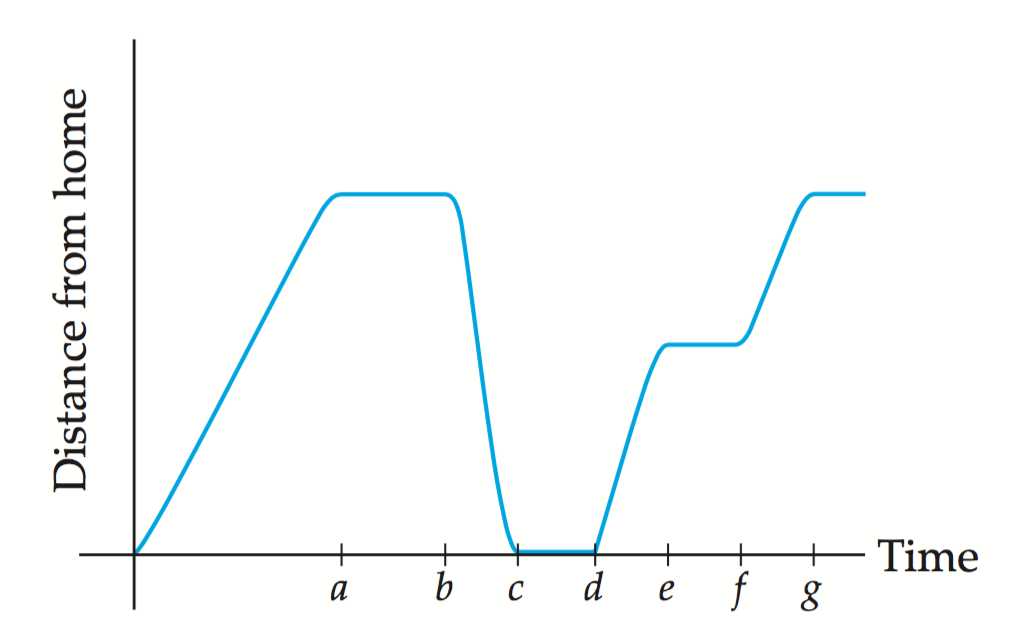
\includegraphics[width=0.7\textwidth]{G9}
	\end{center}
\end{frame}

\begin{frame}
	\frametitle{Edward and Jacob}

	Jacob walked at 5 km/h for 20 minutes and then sprinted at 15 km/h for 8
	minutes.
	\begin{enumerate}
		\item How fast would Edward have to walk or run to go the same distance as Jacob
			did in the same time while moving at a constant speed?

		\item Sketch a graph of Jacob's and Edward's positions over time on the same
			set of axes.
	\end{enumerate}
\end{frame}

\begin{frame}
	\frametitle{Computations: Basic differentiation rules}

	Compute the derivative of the following functions:

	\begin{multicols}{2}
		\begin{enumerate}
			\item $\displaystyle f(x) = x^{100}- 3x^{9}- 2$

			\item $\displaystyle f(x) = \sqrt[3]{x}+ 6$

			\item $\displaystyle f(x) = \frac{4}{x^{4}}$

			\item $\displaystyle f(x) = \sqrt{x}\left( 1 + 2x \right)$

			\item $\displaystyle f(x) = \frac{x^{6}+ 1}{x^{3}}$

			\item $\displaystyle f(x) = \frac{x^{2}-2}{x^{2}+2}$
		\end{enumerate}
	\end{multicols}
\end{frame}

\begin{frame}[t]
	\frametitle{Computations: Chain rule}

	Compute the derivative of

	\begin{enumerate}
		\item $\displaystyle f(x) = \left( 2x^{2}+x+1 \right)^{8}$

		\item $\displaystyle f(x) = \frac{1}{\left( x + \sqrt{x^2+x}\right)^{137}}$
	\end{enumerate}
\end{frame}

\begin{frame}[t]
	\frametitle{A long chain}

	The function below has 137 square roots:
	\[
		f(x) = \sqrt{x+ \sqrt{x +
		\sqrt{x + \sqrt{x+ \ldots + \sqrt{x + \sqrt{x+1}}}}}}
	\]

	Find the equation of the line tangent to the graph of $f$ at the point with
	$x$-coordinate $0$.
\end{frame}

\begin{frame}[t]
	\frametitle{Computations: Trig derivatives}

	Compute the derivatives of the following functions:

	\begin{enumerate}
		%	\item  \DS{f(x) = x \sin x}

		\item $\displaystyle f(x) = \tan (3x^{2}+1)$

			\vfill

		\item $\displaystyle f(x) = (\cos x )( \sin 2x )(\tan 3x)$

			\vfill

		\item $\displaystyle f(x) = \cos ( \sin( \tan x))$
			\vfill

		\item $\displaystyle f(x) = \cos \left( 3x + \sqrt{1 + \sin^{2}x^{2}}\right)$
			\vfill
		%	\item  \DS{f(x) = \frac{x + \sin x}{x + \cos x}}
	\end{enumerate}
\end{frame}

\begin{frame}[t]
	\frametitle{Differentiable functions}

	Let $a \in \mathbb{R}$. \\ Let $f$ be a function with domain $\mathbb{R}$. \\
	Assume $f$ is differentiable everywhere. \\ What can we conclude?

	\begin{multicols}{2}
		\begin{enumerate}
			\item $f(a)$ is defined.

			\item $\displaystyle \lim_{x \to a}f(x)$ exists.

			\item $f$ is continuous at $a$.

			\item $f'(a)$ exists.

			\item $\displaystyle \lim_{x \to a}f'(x)$ exists.

			\item $\displaystyle f'$ is continuous at $a$.
		\end{enumerate}
	\end{multicols}
\end{frame}

\begin{frame}[t]
	\fontsize{13}{13}\selectfont
	\frametitle{True or False - Differentiability vs Continuity}

	Let $f$ be a function with domain $\mathbb{R}$. Let $c \in \mathbb{R}$. \\ Which
	of these implications are true?

	\vfill

	\begin{enumerate}
		\item IF $f$ is {\color{red} continuous} at $c$, THEN $f$ is
			{\color{blue} differentiable} at $c$
			\vfill

		\item IF $f$ is {\color{blue} differentiable} at $c$, THEN $f$ is
			{\color{red} continuous} at $c$
			\vfill

		\item IF $f$ is {\color{blue} differentiable} at $c$, THEN $f'$ is
			{\color{red} continuous} at $c$
			\vfill

		\item IF $f'$ is {\color{red} continuous} at $c$, THEN $f$ is
			{\color{red} continuous} at $c$
			\vfill

		\item IF $f$ is {\color{blue} differentiable} at $c$, THEN $f$ is
			{\color{red} continuous} at and near $c$.
			\vfill

		\item IF $f$ is {\color{red} continuous} at and near $c$, THEN $f$ is
			{\color{blue} differentiable} at $c$.
			\vfill
	\end{enumerate}
\end{frame}

\begin{frame}[t]
	\fontsize{13}{13}\selectfont
	\frametitle{True or False - Differentiability and Operations}

	Let $f$ be a function with domain $\mathbb{R}$. Let $c \in \mathbb{R}$. \\ Let
	$\displaystyle g(x) = f(x)^{2}$. Which of these implications are true?

	\vfill

	\begin{enumerate}
		\item IF $f$ is {\color{blue} differentiable} at $c$, THEN $f+f'$ is
			{\color{red} continuous} at $c$
			\vfill

		\item IF $f$ is {\color{blue} differentiable} at $c$, THEN $3f$ is
			{\color{blue} differentiable} at $c$.
			\vfill

		\item IF $f$ is {\color{blue} differentiable} at $c$, THEN $g$ is
			{\color{blue} differentiable} at $c$.
			\vfill

		\item IF $g$ is {\color{blue} differentiable} at $c$, THEN $f$ is
			{\color{blue} differentiable} at $c$.
			\vfill

		\item IF $f$ is {\color{blue} differentiable} at $c$, THEN $1/f$ is
			{\color{blue} differentiable} at $c$.
			\vfill
	\end{enumerate}
\end{frame}

\begin{frame}[t]
	\frametitle{Vertical things}

	\begin{itemize}
		\item Construct a function $f$ that has a {\color{red} vertical asymptote} at
			$x=2$.

		\item Construct a function $g$ that has a {\color{blue} vertical tangent line}
			at $x=2$.
	\end{itemize}
\end{frame}

\begin{frame}[t]
	\frametitle{Absolute value and tangent lines}

	At (0,0) the graph of $\displaystyle y=|x|$...
	\begin{enumerate}
		\item ... has one tangent line: $y=0$

		\item ... has one tangent line: $x=0$

		\item ... has two tangent lines $y=x$ and $y=-x$

		\item ... has no tangent line
	\end{enumerate}

	\begin{center}
		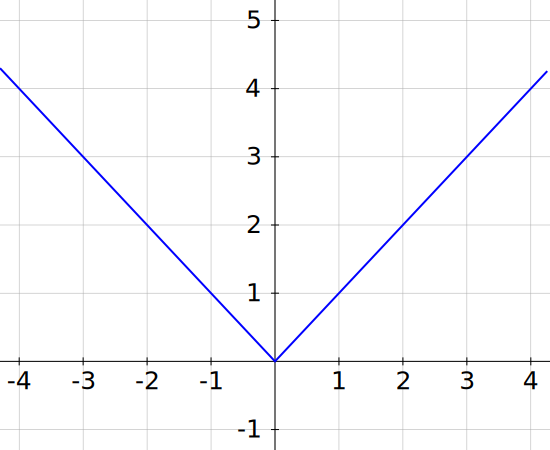
\includegraphics[scale=.25]{G8}
	\end{center}
\end{frame}

\begin{frame}[t]
	\frametitle{Absolute value and derivatives - 1}

	Let $h(x) = x|x|$. What is $h'(0)$?

	\begin{enumerate}
		\item It is 0.

		\item It doesn't exist because $|x|$ is not differentiable at $0$.

		\item It doesn't exist because the right- and left-limits, when computing the
			derivative, are different.

		\item It doesn't exist because it has a corner.

		\item It doesn't exist for a different reason.
	\end{enumerate}
\end{frame}

\begin{frame}[t]
	\frametitle{Absolute value and derivatives - 2}

	\begin{block}{True or False?}
		For all $n \in \mathbb{Z}$ and all $x$, $\frac{d}{dx}|x|^{n}=nx|x|^{n-2}$.
	\end{block}
\end{frame}

\begin{frame}[t]
	\fontsize{13}{13}\selectfont
	\frametitle{Write a proof for the quotient rule for derivatives}

	\begin{block}{Theorem}
		\begin{itemize}
			\item Let $a \in \mathbb{R}$.

			\item Let $f$ and $g$ be functions defined at and near $a$. \\ Assume
				$g(x) \neq 0$ for $x$ close to $a$.

			\item We define the function $h$ by $\displaystyle h(x) = \frac{f(x)}{g(x)}$.
		\end{itemize}

		IF $f$ and $g$ are differentiable at $a$, \\ THEN $h$ is differentiable at $a$,
		and
		\[
			h'(a) = \frac{f'(a) g(a) - f(a) g'(a)}{g(a)^{2}}.
		\]
	\end{block}

	\vfill

	Write a proof directly from the definition of derivative.

	\emph{Hint:} Imitate the proof of the product rule in Video 3.6.
\end{frame}

\begin{frame}[t]
	\frametitle{Check your proof}

	\begin{enumerate}
		\item Did you use the \emph{definition} of derivative?

		\item Are there words or only equations?

		\item Does every step follow logically?

		\item Did you only assume things you could assume?

		\item Did you assume at some point that a function was differentiable? If so,
			did you justify it?

		\item \label{qu:cont} Did you assume at some point that a function was continuous?
			If so, did you justify it?
	\end{enumerate}

	If you answered ``no" to Q\ref{qu:cont}, you probably missed something
	important.
\end{frame}

\begin{frame}[t]
	\fontsize{13}{13}\selectfont
	\frametitle{Critique this proof}
	\vspace{-1cm}
	\begin{align*}
		h'(a) \; & = \; \lim_{x \to a}\frac{h(x) - h(a) }{x - a}\; = \; \lim_{x \to a}\frac{\; \dfrac{f(x)}{g(x)} \; - \; \dfrac{f(a)}{g(a)} \;}{x-a} \\
		\         \\
		         & = \; \lim_{x \to a}\frac{f(x)g(a) - f(a)g(x)}{g(x)g(a) \; (x-a)}                                                                   \\
		\         \\
		         & = \; \lim_{x \to a}\frac{f(x)g(a) - f(a)g(a) + f(a)g(a) - f(a) g(x)}{g(x) g(a) \; (x-a)}                                           \\
		\         \\
		         & = \; \lim_{x \to a}\left\{ \left[ \frac{f(x) - f(a)}{x-a}g(a) - f(a) \frac{g(x) - g(a)}{x-a}\right] \frac{1}{g(x) g(a)}\right\}    \\
		\         \\
		         & = \; \left[ f'(a) g(a) - f(a) g'(a) \right] \frac{1}{g(a) g(a)}
	\end{align*}
\end{frame}

\begin{frame}[t]
	\frametitle{Higher order derivatives}

	Let $\displaystyle g(x) = \frac{1}{x^{3}}$.

	\begin{itemize}
		\item Calculate the first few derivatives.

		\item Make a conjecture for a formula for the $n$-th derivative $\displaystyle
			g^{(n)}(x)$.

		\item Prove it by induction.
	\end{itemize}
\end{frame}

\begin{frame}
	\frametitle{Nixon}

	Richard Nixon, during the 1972 US Presidential campaign, (paraphrased):

	\begin{quote}
		\emph{Inflation is increasing, but the rate of increase of inflation is decreasing.}
	\end{quote}

	\vfill

	Let
	\begin{itemize}
		\item $C$ = cost of life

		\item $t$ = time
	\end{itemize}
	What did Nixon say in terms of derivatives?

	\vfill
\end{frame}

\begin{frame}
	\frametitle{Quick composition}

	Let $f$ and $g$ be differentiable functions and let $h=f\circ g$. \\ What is $h
	^{\prime}(2)$? \begin {enumerate} \item $f^{\prime}(2)\circ g^{\prime}(2)$
	\item $f^{\prime}(2)g^{\prime}(2)$ \item $f^{\prime}(g(2)) g^{\prime}(2)$
	\item $f^{\prime}(g(x)) g^{\prime}(2)$ \end{enumerate}

	%Answer: (c). Even though students may have memorized the Chain Rule formula, some may not be able to apply it to this type of problem.
\end{frame}

\begin{frame}[t]
	\frametitle{True or False - Differentiability and Composition}

	Let $f$ and $g$ be functions with domain $\mathbb{R}$. Let $c \in \mathbb{R}$.
	\\ Assume $f$ and $g$ are differentiable at $c$. \\ What can we conclude?

	\vfill

	\begin{enumerate}
		\item $f \circ g$ \; is {\color{blue} differentiable} at $c$.
			\vfill

		\item $f \circ f$ \; is {\color{blue} differentiable} at $c$.
			\vfill

		\item $f \circ \sin$ \; is {\color{blue} differentiable} at $c$.
			\vfill

		\item $\sin \circ f$ \; is {\color{blue} differentiable} at $c$.
			\vfill
	\end{enumerate}
\end{frame}

\begin{frame}
	\frametitle{Chain rule from a graph}

	If $f$ and $g$ are the functions whose graphs are shown. \\ Let $u(x)=f(g(x))$
	and $v(x)=g(f(x))$. \\
	\medskip

	Find each derivative, if it exists. \\ If it does not exist, explain why.

	\begin{enumerate}
		\item $u'(1)$

		\item $v'(1)$
	\end{enumerate}
	\vspace{-1cm}

	\begin{center}
		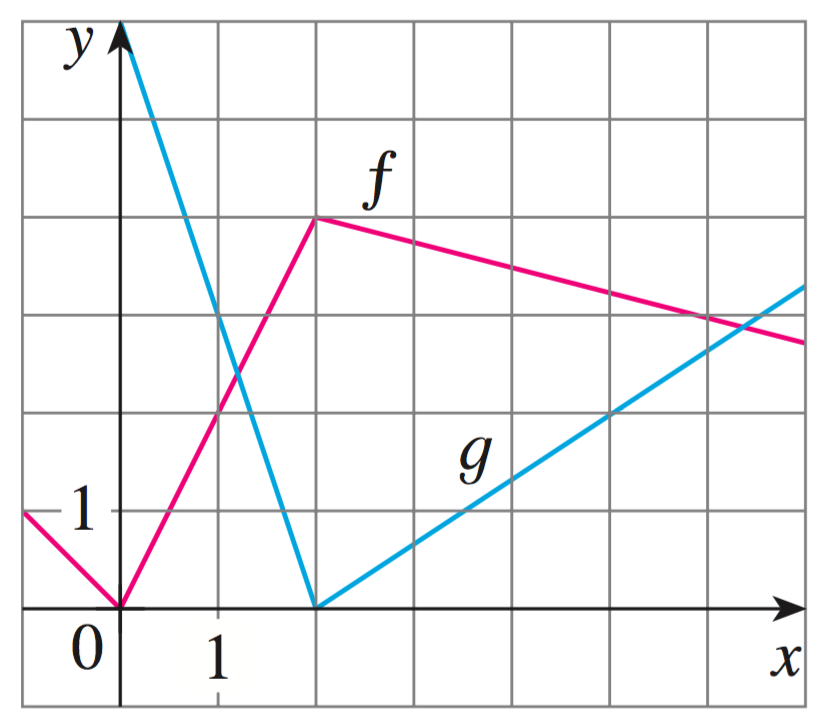
\includegraphics[width=0.5\textwidth]{G10}
	\end{center}
\end{frame}

\begin{frame}[t]
	\frametitle{Balloon}

	I am inflating a spherical balloon. Below is the graph of the radius $r$ (in
	$cm$) as a function of time $t$ (in $s$). At what rate is the volume of the
	balloon increasing at time $4s$?

	\begin{center}
		\only<1>{
		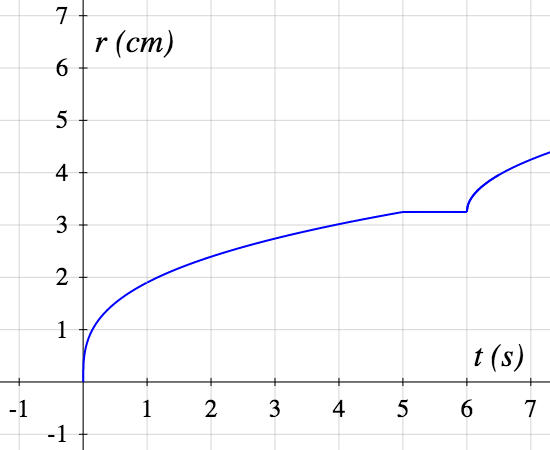
\includegraphics[scale=.35]{G6}
		} \only<2>{
		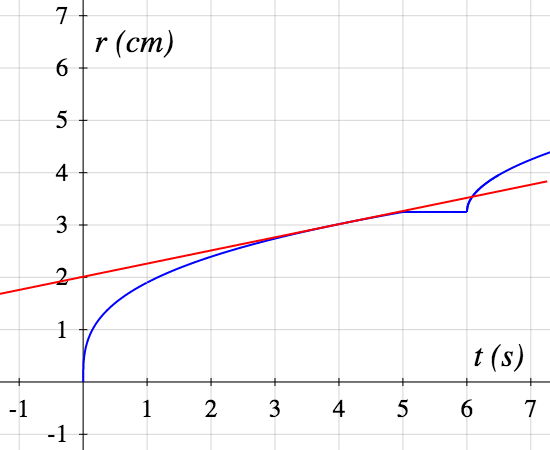
\includegraphics[scale=.35]{G7}
		}
	\end{center}
\end{frame}

\begin{frame}[t]
	\frametitle{An alternative proof of the quotient rule}

	Assume we have already proven the product rule, the power rule, and the chain
	rule.

	Obtain a formula for the derivative of
	$\displaystyle h(x) = \frac{f(x)}{g(x)}$.

	\emph{Hint:} $\displaystyle \frac{f(x)}{g(x)}= f(x) \cdot g(x)^{-1}$
\end{frame}

\begin{frame}
	\frametitle{Derivatives of $\displaystyle (f \circ g)$}

	Assume $f$ and $g$ are functions that have all their derivatives. Find formulas
	for
	\begin{enumerate}
		\item $\displaystyle (f \circ g)'(x)$

		\item $\displaystyle (f \circ g)''(x)$

		\item $\displaystyle (f \circ g)'''(x)$
	\end{enumerate}

	in terms of the values of $f$, $g$ and their derivatives.

	\emph{Hint:} The first one is simply the chain rule.

	\
	% \pause

	\emph{Challenge:} Find a formula for $\displaystyle (f \circ g)^{(n)}(x)$ \\ (This
	is beyond the scope of this course).
\end{frame}

\begin{frame}[t]
	\frametitle{Derivative of $\cos$}

	Let $\displaystyle g(x) = \cos x.$

	Obtain and prove a formula for its derivative directly from the definition of derivative
	as a limit.

	\vfill

	{\bfseries Hint:} Imitate the derivation in Video 3.12. \\ If you need a trig identity
	that you do not know, google it or ask another student.

	%{\bf Hint:}  This identity may come in handy:

	%	$$

	%		\cos (a + b) = \cos a \cos b - \sin a \sin b

	%	$$
\end{frame}

\begin{frame}[t]
	\frametitle{Derivatives of the other trig functions}

	Use the basic differentiation rules, as well as
	\[
		\frac{d}{dx}\sin x = \cos x, \quad \quad \frac{d}{dx}\cos x = - \sin x,
	\]
	to quickly obtain and prove formulas for the derivatives of $\tan$, $\cot$, $\sec$,
	and $\csc$.
\end{frame}

\begin{frame}
	\frametitle{Product of trig functions}

	Let $f(x)= \sin x \cos x$. What is its derivative $f'(x)$?
	\begin{enumerate}
		\item $1-2\sin^{2}(x)$

		\item $2\cos^{2}(x) -1$

		\item $\cos 2x$

		\item all of the above

		\item none of the above
	\end{enumerate}

	%Answer: (d).} (a) - (c) are equivalent formulae. One can get (a) by using the product rule and $\cos^2(x)=1-\sin ^2(x)$.
\end{frame}

\begin{frame}[t]
	\frametitle{A pesky function}

	Let $\displaystyle h(x) =
	\begin{cases}
		x^{2}\sin \dfrac{\;1\;}{x} & \text{ if }x \neq 0 \\
		0                          & \text{ if }x=0
	\end{cases}$.

	\begin{enumerate}
		\item Calculate $\displaystyle h'(x)$ for any $x \neq 0$.

		\item \label{it:0a} Using the definition of derivative, calculate
			$\displaystyle h'(0)$.

		\item \label{it:0b} Calculate $\displaystyle \lim_{x \to 0}h'(x)$

			\vspace{.2cm}
			{\fontsize{13}{13}\selectfont \emph{Hint:} Questions \ref{it:0a} and \ref{it:0b} have different answers.}

			% \pause
			\vspace{.2cm}

		\item Is $h$ continuous at $0$?

		\item Is $h$ differentiable at $0$?

		\item Is $h'$ continuous at $0$?
	\end{enumerate}
\end{frame}

\begin{frame}[t]
	\frametitle{Implicit differentiation}

	The equation
	\[
		\sin (x+y) + xy^{2}= 0
	\]
	defines a function $\displaystyle y=h(x)$ near $(0,0)$. \href{https://www.desmos.com/calculator/bvupq00r6s}{\beamergotobutton{graph}}

	Using implicit differentiation, compute
	\begin{multicols}{4}
		\begin{enumerate}
			\item $\displaystyle h(0)$

			\item $\displaystyle h'(0)$

			\item $\displaystyle h''(0)$

			\item $\displaystyle h'''(0)$
		\end{enumerate}
	\end{multicols}
\end{frame}

\begin{frame}[t]
	\frametitle{Worm up}

	% Why this question?  Some students will answer ``False" because ``the graph crosses itself"

	A worm is crawling accross the table. The path of the worm looks something
	like this:

	%\vspace{-1cm}

	\begin{center}
		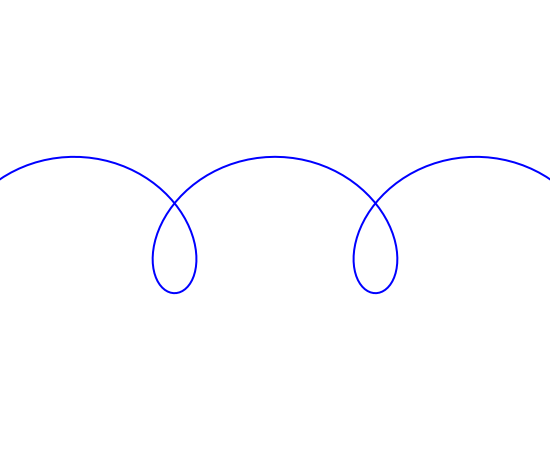
\includegraphics[scale=.3]{G11}
	\end{center}

	\vspace{-1cm}

	\begin{block}{True or False?}
		The position of the worm is a function.
	\end{block}
\end{frame}

\begin{frame}[t]
	\frametitle{Worm function}

	\vspace{-.7cm}

	\begin{center}
		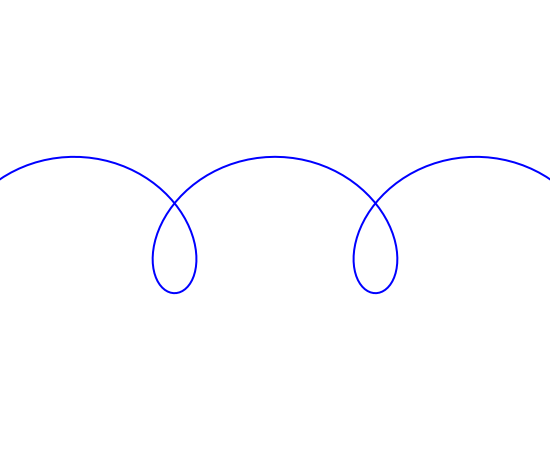
\includegraphics[scale=.3]{G11}
	\end{center}

	\vspace{-1.5cm}

	A worm is crawling accross the table. \\ For any time $t$, let $f(t)$ be the position
	of the worm. \\ This defines a function $f$.

	\begin{enumerate}
		\item What is the domain of $f$?

		\item What is the codomain of $f$?

		\item What is the range of $f$?
	\end{enumerate}
\end{frame}

\begin{frame}
	\frametitle{\small Finding a Restricted Domain on which a Function is
	Invertible}
	\vspace{-3mm}
	%\begin{minipage}{0.35\textwidth}
	\begin{center}
		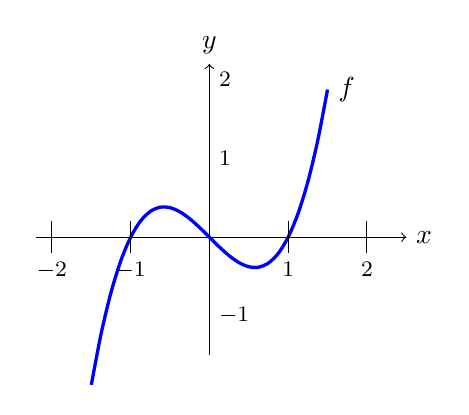
\begin{tikzpicture}[scale=1]
			\draw[->] (-2.2,0) -- (2.5,0) node[right] {$x$};
			\draw[->] (0,-1.5) -- (0,2.2) node[above] {$y$};
			\draw[
				draw=blue,
				very thick,
				scale=1,
				domain=-1.5:1.5,
				smooth,
				variable=\x
			] plot (\x,\x*\x*\x-\x) node[right] {$f$};

			\node[below] at (-2,-0.2) {\footnotesize $-2$};
			\node[below] at (-1,-0.2) {\footnotesize$-1$};
			%\node [below] at (0,0) {\footnotesize$0$};
			\node[below] at (1,-0.2) {\footnotesize$1$};
			\node[below] at (2,-0.2) {\footnotesize$2$};
			%

			%\node [right] at (0,-2) {\footnotesize$-2$};
			\node[right] at (0,-1) {\footnotesize$-1$};
			\node[right] at (0,1) {\footnotesize$1$};
			\node[right] at (0,2) {\footnotesize$2$};

			\draw (1,-0.2) -- (1,0.2);
			\draw (2,-0.2) -- (2,0.2);
			\draw (-1,-0.2) -- (-1,0.2);
			\draw (-2,-0.2) -- (-2,0.2);
		\end{tikzpicture}
	\end{center}
	%		\end{minipage}

	%		%%%%%%%%

	%\begin{minipage}{0.6\textwidth}
	\begin{enumerate}
		\item Find the largest interval containing 0 on which $f$ is invertible.

		\item Find the largest interval containing 1 on which $f$ is invertible.
	\end{enumerate}
\end{frame}

\begin{frame}
	\frametitle{Fill in the Blank }

	Given that $f$ is an invertible function, fill in the blanks.
	\begin{enumerate}
		\item If $f(-1) = 0$, then $f^{-1}(0) =$ ------.

		\item If $f^{-1}(2) = 1$, then $f(1)=$ ------.

		\item If $(2,3)$ is on the graph of $f$, then ------ is on the graph of $f^{-1}$.

		\item If ------ is on the graph of $f$, then $(-2,4)$ is on the graph of $f^{-1}$.
	\end{enumerate}
\end{frame}

\begin{frame}
	\frametitle{Inverse function from a graph}

	\begin{columns}[c]
		\column{.65\textwidth}
		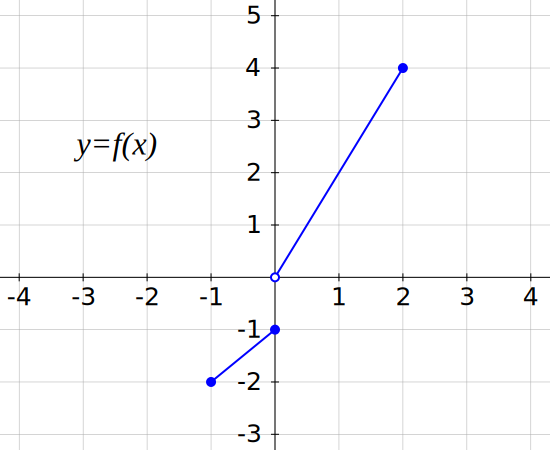
\includegraphics[scale=.4]{G12}
		\column{.3\textwidth}
		Calculate:
		\begin{enumerate}
			\item $\displaystyle f(2)$

			\item $\displaystyle f(0)$

			\item $\displaystyle f^{-1}(2)$

			\item $\displaystyle f^{-1}(0)$

			\item $\displaystyle f^{-1}(-1)$
		\end{enumerate}
	\end{columns}
\end{frame}

\begin{frame}[t]
	\frametitle{Absolute value and inverses}

	Let
	\[
		h(x) = x |x| + 1
	\]
	\begin{enumerate}
		\item Calculate $\displaystyle h^{-1}(-8)$.
		% \pause

		\item Sketch the graph of $h$.

		\item Find an equation for $\displaystyle h^{-1}$.

		\item Sketch the graph of $\displaystyle h^{-1}$.

		\item Verify that
			\begin{itemize}
				\normalsize

				\item for every $\displaystyle t \in \boxed{???}$, \;
					$\displaystyle h(h^{-1}(t)) = t$.

				\item for every $\displaystyle t \in \boxed{???}$, \;
					$\displaystyle h^{-1}(h(t)) = t$.
			\end{itemize}
	\end{enumerate}
\end{frame}

\begin{frame}[t]
	\frametitle{Functions, inverses, and graphs }

	Sketch the graph of a function $g$ satisfying all the following properties:

	\begin{enumerate}
		\item The domain of $g$ is $\mathbb{R}$.

		\item $g$ is continuous everywhere except at $-2$.

		\item $g$ is differentiable everywhere except at $-2$ and $1$.

		\item $g$ has an inverse function.

		\item $g(0)=2$

		\item $g'(0) = 2$

		\item $\displaystyle \left(g^{-1}\right)' (-3) = -2$.
	\end{enumerate}
\end{frame}

\begin{frame}[t]
	\frametitle{Functions, inverses, and graphs - 2}
	%This appeared in a past test

	Draw the graph of a function $f$ satisfying all of the following:

	\begin{enumerate}
		\item The domain of $f$ is $\mathbb{R}$.

		\item $f$ is differentiable everywhere.

		\item The restriction of $f$ to $\displaystyle [0, \infty)$ is one-to-one,
			\\ and its INVERSE has a vertical tangent line at $2$.

		\item The restriction of $f$ to $\displaystyle (- \infty,0]$ is one-to-one,
			\\ and its INVERSE has derivative $2$ at $2$.
	\end{enumerate}
\end{frame}

\begin{frame}[t]
	\frametitle{Composition and inverses}

	Assume for simplicity that all functions in this problem have domain
	$\mathbb{R}$.

	\vfill

	Let $f$ and $g$ be functions. Assume they each have an inverse.

	\vfill

	Is $\displaystyle \left( f \circ g \right)^{-1}= f^{-1}\circ g^{-1}$?

	\begin{itemize}
		\item If YES, prove it.

		\item If NO, fix the statement.
	\end{itemize}

	\vfill
	% \pause

	If you do not know how to start, experiment with the functions
	\[
		f(x) = x + 1, \quad \quad g(x) = 2x.
	\]
\end{frame}

\begin{frame}[t]
	\frametitle{Composition of one-to-one functions}

	Assume for simplicity that all functions in this problem have domain
	$\mathbb{R}$. Prove the following theorem.

	\vfill

	\begin{block}{Theorem A}
		Let $f$ and $g$ be functions. \\ IF $f$ and $g$ are one-to-one, \\ THEN $f \circ
		g$ is one-to-one.
	\end{block}

	\vfill

	% \pause
	Suggestion:
	\begin{enumerate}
		\item Write the definition of what you want to prove.

		\item Figure out the formal structure of the proof.

		\item Complete the proof (use the hypotheses!)
	\end{enumerate}
\end{frame}

\begin{frame}[t]
	\frametitle{Composition of one-to-one functions -- 2}

	Assume for simplicity that all functions in this problem have domain
	$\mathbb{R}$. Prove the following theorem.

	\begin{block}{Theorem B}
		Let $f$ and $g$ be functions. \\ IF $f \circ g$ is one-to-one, \quad THEN $g$
		is one-to-one.
	\end{block}

	% \pause
	Suggestion:
	\begin{enumerate}
		\item Transform the ``$\displaystyle P \implies Q$'' theorem into an equivalent
			``$\displaystyle \text{(not Q)}\implies \text{(not P)}$'' theorem. \\ You
			will prove that one instead.
		% \pause

		\item Write the definition of the hypotheses \\ and of the conclusion.

		\item Write the proof.
	\end{enumerate}
\end{frame}

\begin{frame}[t]
	\frametitle{Composition of one-to-one functions -- 3}

	Assume for simplicity that all functions in this problem have domain
	$\mathbb{R}$.

	\vfill

	Prove the following claim is FALSE with a counterexample.

	\vfill

	\begin{block}{Claim }
		Let $f$ and $g$ be functions. \\ IF $f \circ g$ is one-to-one, \\ THEN $f$ is
		one-to-one.
	\end{block}

	\vfill
\end{frame}

\begin{frame}[t]
	\frametitle{Increasing and one-to-one}

	\begin{block}{Definition}
		Let $f$ be a function with domain $D$. We say that $f$ is \emph{increasing} on
		$D$ when

		\[
			\forall x_{1}, x_{2}\in D, \quad x_{1}<x_{2}\implies f(x_{1})<f(x_{2}).
		\]
	\end{block}

	\begin{enumerate}
		\item Prove that if a function is increasing, then it is one-to-one.
		% \pause

		\item Use this to show that $g(x) = x^{5}+ 4x^{3}+ 2x + 1$ has an inverse.

		\item Find $(g^{-1})'(1)$.
	\end{enumerate}
\end{frame}

\begin{frame}[t]
	\frametitle{Where is the error?}

	\begin{itemize}
		\item We know that \boxed{{\color{blue} (f^{-1})' = \frac{1}{f'}}}

		\item Let $\displaystyle f(x) = x^{2}$, restricted to the domain
			$\displaystyle x \in (0, \infty)$
			\[
				f'(x) = 2x \quad \text{and}\quad \boxed{{\color{red} f'(4) = 8}}
			\]

		\item Then $\displaystyle f^{-1}(x) = \sqrt{x}$
			\[
				(f^{-1})'(x) = \frac{1}{2\sqrt{x}}\quad \text{ and }\quad \boxed{{\color{red} (f^{-1})'(4) = \frac{1}{4}}}
			\]

		\item So \boxed{{\color{blue} (f^{-1})'(4) \neq \frac{1}{f'(4)}}}
	\end{itemize}
\end{frame}

\begin{frame}[t]
	\frametitle{Derivatives of the inverse function}

	Let $f$ be a one-to-one function. \\ Let $a, b \in \mathbb{R}$ such that $b=f(a
	)$.

	\vfill
	\begin{enumerate}
		\item Obtain a formula for $\displaystyle \left(f^{-1}\right)'(b)$ in terms of
			$\displaystyle f'(a)$.
			\vspace{.2cm}

			{\fontsize{13}{13}\selectfont \emph{Hint:} This was done in Video 4.4 \\ Take $\displaystyle \frac{d}{dy}$ of both sides of \quad $\displaystyle f(f^{-1}( (y)) = y$. }

			% \pause
			\vfill

		\item Obtain a formula for $\displaystyle \left(f^{-1}\right)''(b)$ in terms
			of $\displaystyle f'(a)$ and $\displaystyle f''(a)$.

			% \pause
			\vfill

		\item \emph{Challenge:} Obtain a formula for
			$\displaystyle \left(f^{-1}\right)'''(b)$ in terms of
			$\displaystyle f'(a)$, $\displaystyle f''(a)$, and $\displaystyle f'''(a)$.
	\end{enumerate}
\end{frame}

\begin{frame}[t]
	\frametitle{Computations - Exponentials and logarithms}

	Compute the derivative of the following functions:

	\begin{enumerate}
		\item $\displaystyle f(x) = e^{\sin x + \cos x}\ln x$
			\vfill

		\item $\displaystyle f(x) = \pi^{\tan x}$
			\vfill

		\item $\displaystyle f(x) = \ln \left[ e^{x}+ \ln \ln \ln x \right]$
			\vfill

		\item $\displaystyle f(x) = \log_{10}\left( 2x + 3 \right)$
			\vfill
	\end{enumerate}
\end{frame}

\begin{frame}[t]
	\frametitle{Logarithm and Absolute Value}

	The function $F$ is defined by the equation
	\[
		F(x) = \ln |x| .
	\]
	What is its derivative?
	\vfill
	\begin{enumerate}
		\item $\displaystyle F'(x) = \frac{1}{x}$
			\vfill

		\item $\displaystyle F'(x) = \frac{1}{|x|}$
			\vfill

		\item $F$ is not differentiable
			\vfill
	\end{enumerate}
\end{frame}

\begin{frame}[t]
	\frametitle{A different type of logarithm}

	Calculate the derivative of
	\[
		f(x) = \log_{x+1}(x^{2}+1)
	\]

	\vfill

	\emph{Note:} This is a new function. We have not given you a formula for it
	yet, That is on purpose.

	\vfill
	% \pause

	\emph{Hint:} If you do not know where to start, remember the definition of
	logarithm:
	\[
		\log_{a}b = c \; \iff \; a^{c}= b.
	\]
\end{frame}

\begin{frame}[t]
	\frametitle{Logarithmic differentiation}

	\vspace{5mm}
	\begin{block}{}
		Calculate the derivative of
		\[
			g(x) = x^{\tan x}.
		\]
	\end{block}
\end{frame}

\begin{frame}[t]
	\fontsize{13}{13}\selectfont
	\frametitle{More logarithmic differentiation}

	\begin{block}{}
		Calculate the derivative of
		\[
			f(x) = \left( \sin x \right)^{\cos x}+ \left( \cos x \right)^{\sin x}.
		\]
	\end{block}

	% \pause
	\vfill

	{\bfseries \underline{What is wrong with this answer?}}
	\begin{align*}
		\ln f(x) =                                          & (\cos x) \ln ( \sin x )+ ( \sin x ) ( \ln \cos x )                                                                                   \\
		{\color{red} \frac{d}{dx}}\left[ \ln f(x) \right] = & {\color{red} \frac{d}{dx}}\left[ (\cos x) \ln ( \sin x ) \right] +{\color{red} \frac{d}{dx}}\left[ ( \sin x ) ( \ln \cos x ) \right] \\
		\frac{f'(x)}{f(x)}=                                 & - ( \sin x ) \ln (\sin x) + (\cos x ) \frac{\cos x}{\sin x}                                                                          \\
		                                                    & + ( \cos x ) \ln (\cos x) + (\sin x ) \frac{- \sin x}{\cos x}
	\end{align*}
	\[
		{f'(x) = f(x) \left[ - (\sin x) \ln(\sin x) + (\cos x) \ln (\cos x) + \frac{\cos^{2}x}{\sin x} - \frac{\sin^{2}x}{\cos x} \right]}
	\]
\end{frame}

\begin{frame}[t]
	\frametitle{Hard derivatives made easier}

	\vspace{5mm}
	\begin{block}{}
		Calculate the derivative of
		\[
			h(x) = \sqrt[3]{\frac{\left( \sin^{6}x \right) \sqrt{x^7+6x+2}}{3^{x}\left(x^{10}+2x\right)^{10}}}
		\]
	\end{block}
\end{frame}

\begin{frame}[t]
	\frametitle{An Implicit Function}

	\vspace{5mm}
	\begin{block}{}
		Find $y'$ if $x^{y}=y^{x}$.
	\end{block}
\end{frame}

\begin{frame}[t]
	\fontsize{13}{13}\selectfont
	\frametitle{Definition of $\arctan$}

	\begin{enumerate}
		\item Sketch the graph of $\tan$.

		\item Prove that $\tan$ is not one-to-one.

		\item Select the largest interval containing $0$ such that the restriction of
			$\tan$ to it is one-to-one. We define $\arctan$ as the inverse of this
			restriction. \quad Let $x, y \in \mathbb{R}$
			%	\item
			\[
				\arctan y = x \; \quad \; \iff \; \quad ???
			\]

		\item What is the domain of $\displaystyle \arctan$? What is the range of
			$\displaystyle \arctan$?

			Sketch the graph of $\arctan$.

		\item Compute
			\begin{multicols}{2}
				\begin{enumerate}
					\item $\displaystyle \arctan \left( \tan \left( 1 \right) \right)$

					\item $\displaystyle \arctan \left( \tan \left( 3\right) \right)$

					\item $\displaystyle \arctan \left( \tan \left( \frac{\pi}{2}\right) \right
						)$

					\item $\displaystyle \arctan \left( \tan \left( -6)\right) \right)$

					\item $\displaystyle \tan \left( \arctan \left( 0\right) \right)$

					\item $\displaystyle \tan \left( \arctan \left( 10\right) \right)$
				\end{enumerate}
			\end{multicols}
	\end{enumerate}
\end{frame}

\begin{frame}[t]
	\frametitle{Derivative of $\arctan$}

	\begin{block}{}
		Obtain (and prove) a formula for the derivative of $\arctan$.
	\end{block}

	\emph{Hint:} Call $\displaystyle f(t) = \arctan t$ and differentiate
	\[
		\forall t \in \ldots \quad \quad \tan ( f(t)) = t
	\]
\end{frame}

\begin{frame}[t]
	\frametitle{Computations - Inverse trig functions}

	Compute the derivatives of these functions, and simplify them as much as possible:
	\begin{enumerate}
		\item $\displaystyle f(x) = \arcsin \left( x^{3/2}\right)$
			\vfill

		\item $\displaystyle f(x)=2x^{2}\arctan (x^{2}) - \ln (x^{4}+1)$
			\vfill
	\end{enumerate}
\end{frame}

\begin{frame}[t]
	\frametitle{Trig-inverse-trig}

	\begin{block}{}
		Find simple expressions for these quantities and state the domain on which they
		are valid:
		\begin{enumerate}
			\begin{multicols}{2}
				\item $\displaystyle \sin \; ( \arccos x)$ \item $\displaystyle \sec \; (
				\arccos x)$ \item $\displaystyle \sec \; ( \arctan x)$ \item $\displaystyle
				\tan \; (\operatorname{arcsec}x)$
			\end{multicols}
		\end{enumerate}
		\vspace{-.1cm}
	\end{block}

	\
	% \pause

	{\fontsize{13}{13}\selectfont \emph{Hint:} There are two standard ways to attack these problems: \begin{itemize}\item Use a trig identity \\ e.g.: a trig identity relating $\sin$ and $\cos$ for (1)

	\item Or draw a right triangle with side lengths $1$ and $x$ \\ e.g.: with an angle $\theta$ such that $\cos \theta = x$ for (1)\end{itemize} If you need to take a square root, you must justify which branch ($+$ or $-$) you are choosing. }
\end{frame}

\begin{frame}[t]
	\frametitle{$\operatorname{arcsec}$}

	\begin{enumerate}
		\item Complete: ``We define $\operatorname{arcsec}$ as the inverse of the
			restriction of $\sec$ to ..."

			\emph{Hint:} Sketch the graph of $\sec$.

			\vfill

		\item What are the domain and range of $\operatorname{arcsec}$? \\ Sketch
			its graph.

			\vfill

		\item Obtain (and prove) a formula for the derivative of $\operatorname{arcsec}$
			in the same way you did for $\arctan$.

			\vfill

		\item Now obtain the same formula in a different way: use
			$\displaystyle \sec x = \frac{1}{\cos x}$ to write
			$\displaystyle \operatorname{arcsec}$ in terms of $\displaystyle \arccos$.
	\end{enumerate}
\end{frame}

\begin{frame}
	\frametitle{Definition of local extremum}

	Find local and global extrema of the function with this graph:

	\begin{center}
		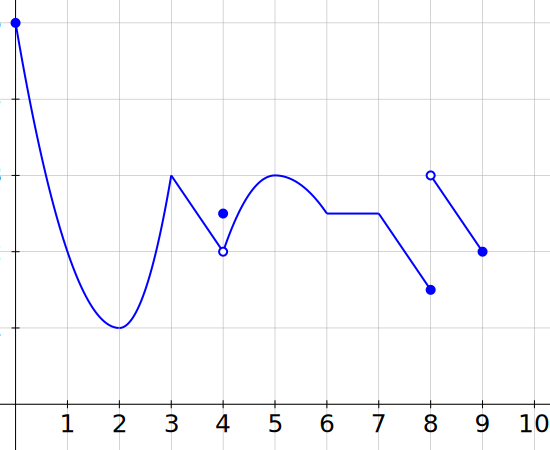
\includegraphics[scale=.42]{G13}
	\end{center}
\end{frame}

\begin{frame}[t]
	\frametitle{Where is the maximum?}

	We know the following about the function $h$:
	\begin{itemize}
		\item The domain of $h$ is $\displaystyle (-4,4)$.

		\item $h$ is continuous on its domain.

		\item $h$ is differentiable on its domain, except at $0$.

		\item $h'(x) = 0 \quad \iff \quad x=-1 \text{ or }1$.
	\end{itemize}

	\begin{block}{What can you conclude about the maximum of $h$?}
		% \pause
		\begin{enumerate}
			\item $h$ has a maximum at $x=-1$, or $1$.

			\item $h$ has a maximum at $x=-1,0,$ or $1$.

			\item $h$ has a maximum at $x=-4, -1,0, 1,$ or $4$.

			\item None of the above.
		\end{enumerate}
	\end{block}
\end{frame}

\begin{frame}[t]
	\frametitle{What can you conclude?}

	We know the following about the function $f$.
	\begin{itemize}
		\item $f$ has domain $\mathbb{R}$.

		\item $f$ is continuous

		\item $f(0)=0$

		\item For every $x \in \mathbb{R}$, $f(x) \geq x$.
	\end{itemize}
	\begin{block}{}
		What can you conclude about $f'(0)$? Prove it.
	\end{block}

	\vfill

	\emph{Hint:} Sketch the graph of $f$. Looking at the graph, make a conjecture.
	\\ To prove it, imitate the proof of the Local EVT from Video 5.3.
\end{frame}

\begin{frame}[t]
	\frametitle{Fractional exponents}

	Let $\displaystyle g(x) = x^{2/3}(x-1)^{3}.$

	Find local and global extrema of $g$ on $\displaystyle [-1,2]$.
\end{frame}

\begin{frame}[t]
	\frametitle{Trig extrema}

	Let $\displaystyle f(x) = \frac{\sin x}{3 + \cos x}.$

	Find the maximum and minimum of $f$.
\end{frame}

\begin{frame}[t]
	\frametitle{How many zeroes?}

	Let
	\[
		f(x) = e^{x}- \sin x + x^{2}+ 10x
	\]

	How many zeroes does $f$ have?
\end{frame}

\begin{frame}[t]
	\frametitle{Zeroes of the derivative}

	Sketch the graph of a function $f$ that is differentiable on $\mathbb{R}$ and
	such that

	\begin{enumerate}
		\item $f$ has exactly 3 zeroes and $f'$ has exactly 2 zeroes.

		\item $f$ has exactly 3 zeroes and $f'$ has exactly 3 zeroes.

		\item $f$ has exactly 3 zeroes and $f'$ has exactly 1 zero.

		\item $f$ has exactly 3 zeroes and $f'$ has infinitely many zeroes.
	\end{enumerate}
\end{frame}

\begin{frame}[t]
	\frametitle{Zeroes of a polynomial}

	You probably learned in high school that a polynomial of degree $n$ has at
	most $n$ real zeroes. Now you can prove it!

	\emph{Hint:} Use induction. If you are having trouble, try the case $n=3$
	first.
\end{frame}

\begin{frame}[t]
	\frametitle{The second Theorem of Rolle}

	Complete statement for this theorem and prove it.

	\vfill

	\begin{block}{Rolle's Theorem 2}
		Let $a<b$. Let $f$ be a function defined on $[a,b]$. \\ IF
		\begin{itemize}
			\item (Some conditions on continuity and derivatives)

			\item $\displaystyle f(a) = f'(a) =0$

			\item $\displaystyle f(b)=0$
		\end{itemize}
		THEN $\displaystyle \exists c \in (a,b)$ such that $\displaystyle f''(c)=0$.
	\end{block}

	\vfill

	\emph{Hint:} Apply the 1st Rolle's Theorem to $f$, then do something else.
\end{frame}

\begin{frame}[t]
	\frametitle{The $N$-th Theorem of Rolle}

	Complete the statement for this theorem and prove it.

	\begin{block}{Rolle's Theorem $N$}
		Let $N$ be a positive integer. \\ Let $a<b$. Let $f$ be a function defined on
		$[a,b]$. \\ IF
		\begin{itemize}
			\item (Some conditions on continuity and derivatives)

			\item (Some conditions at $a$)

			\item $\displaystyle f(b)=0$
		\end{itemize}
		THEN $\displaystyle \exists c \in (a,b)$ such that
		$\displaystyle f^{(N)}(c)=0$.
	\end{block}
\end{frame}

\begin{frame}[t]
	\fontsize{13}{13}\selectfont
	\frametitle{A new theorem}

	We want to prove this theorem:
	\begin{block}{\fontsize{13}{13}\selectfont Theorem 1}
		Let $f$ be a differentiable function on an open interval $I$. \\ IF
		$\displaystyle \forall x \in I, f'(x) \neq 0$ \\ THEN $f$ is one-to-one on
		$I$.
	\end{block}

	\vfill
	% \pause

	\begin{enumerate}
		\item Transform \quad $\displaystyle [P \implies Q]$ \quad into \quad $\displaystyle
			[(\text{not }Q) \implies (\text{not }P)]$. \\ You get an equivalent
			Theorem (call it ``Theorem 2"). \\ We are going to prove Theorem 2 instead.

		\item Write the definition of ``$f$ is not one-to-one on $I$". You will need
			it.

		\item Recall the statement of Rolle's Theorem. You will need it.

		\item Do some rough work if needed.

		\item Write a complete proof for Theorem 2.
	\end{enumerate}
\end{frame}

\begin{frame}[t]
	\frametitle{A variant}

	Complete this variation on Theorem 2. \\ Use the weakest conditions you can to
	make it true.

	\begin{block}{Theorem 3}
		Let $a<b$. Let $f$ be a function defined on $[a,b]$. \\ IF
		\begin{itemize}
			\item (Some conditions on continuity and differentiability)

			\item $f$ is not one-to-one on $[a,b]$
		\end{itemize}
		THEN $\displaystyle \exists c \in (a,b)$ such that $f'(c)=0$.
	\end{block}
\end{frame}

\begin{frame}
	\frametitle{Why the three hypotheses are necessary}

	You have proven

	\begin{block}{Theorem 3}
		Let $a<b$. Let $f$ be a function defined on $[a,b]$. \\ IF
		\begin{enumerate}
			\item $f$ is continuous on $[a,b]$

			\item $f$ is differentiable on $(a,b)$

			\item $f$ is not one-to-one on $[a,b]$
		\end{enumerate}
		THEN $\displaystyle \exists c \in (a,b)$ such that $f'(c)=0$.
	\end{block}

	\vfill

	Give three examples to justify that each of the three hypotheses are necessary
	for the theorem to be true. (Graphs of the examples are enough).
\end{frame}

\begin{frame}[t]
	\frametitle{MVT -- True or False?}

	\begin{block}{True or False}
		Consider $f(x) = |x|$ on the interval $[-\frac{1}{2}, 2]$.

		There exists $c$ in $(-\frac{1}{2},2)$ such that
		\[
			f'(c) = \frac{f(2) - f(-\frac{1}{2})}{2-(-\frac{1}{2})}
		\]
	\end{block}
	%This is a quick warm up question to make sure that students watched the video and understand that we need to check that all the hypotheses are satisfied before using the theorem.
\end{frame}

\begin{frame}[t]
	\fontsize{13}{13}\selectfont
	\frametitle{Car race - 1}

	A driver competes in a race.

	Use MVT to prove that at some point during the race the instantaneous velocity
	of the driver is exactly equal to the average velocity of the driver during the
	race.
\end{frame}

\begin{frame}[t]
	\fontsize{13}{13}\selectfont
	\frametitle{Car race - 2}

	Two drivers start a race at the same moment and finish in a tie.

	Can you conclude that there was a time in the race (not counting the starting
	time) when the two drivers had exactly the same speed?
\end{frame}

\begin{frame}[t]
	\fontsize{13}{13}\selectfont
	\frametitle{Car race - Is this proof correct?}

	\begin{block}{\fontsize{13}{13}\selectfont Claim}
		IF two drivers start a race at the same moment and finish in a tie, THEN at
		some point in the race (not counting the starting time) they had exactly the
		same speed.
	\end{block}

	{\bfseries Proof?}
	\begin{itemize}
		\item Let $f(t)$ and $g(t)$ be the positions of the two cars at time $t$.

		\item Assume the race happens in the interval $[t_{1},t_{2}]$. By hypothesis:
			\[
				f(t_{1}) = g(t_{1}), \quad \quad f(t_{2}) = g(t_{2}).
			\]

		\item Using MVT, there exists $c \in (t_{1}, t_{2})$ such that
			\[
				f'(c) = \frac{f(t_{2}) - f(t_{1})}{t_{2}- t_{1}}, \quad g'(c) = \frac{g(t_{2})
				- g(t_{1})}{t_{2}- t_{1}}.
			\]

		\item Then $f'(c) = g'(c)$. \hfill $\square$
	\end{itemize}
\end{frame}

\begin{frame}[t]
	\fontsize{13}{13}\selectfont
	\frametitle{Car race - resolution}

	Two drivers start a race at the same moment and finish in a tie.

	Prove that at some point during the race (not counting the starting time) the two
	drivers had exactly the same speed.
\end{frame}

\begin{frame}[t]
	\fontsize{13}{13}\selectfont
	\frametitle{Speeding ticket!}

	On a toll road Barney takes a time stamped toll-card from the starting booth and
	drives directly to the end of the toll section. \\
	\vspace{.2cm}

	After paying the required toll, Barney is surprised to receive a speeding
	ticket along with the toll receipt. \\
	\vspace{.2cm}

	Which of the following are true?
	\vspace{.2cm}
	\begin{enumerate}
		\item The booth attendant does not have enough information to prove that Barney
			was speeding.

		\item The booth attendant can prove that Barney was speeding during his trip.

		\item Barney's ticket is for a lower speed than his actual maximum speed.
	\end{enumerate}
\end{frame}

\begin{frame}[t]
	\frametitle{Proving difficult identities}

	\begin{block}{}
		Prove that, for every $x \geq 0$,
		\[
			2 \arctan \sqrt{x}- \arcsin \frac{x-1}{x+1}= \frac{\pi}{2}
		\]
	\end{block}

	\emph{Hint:} Derivatives.
\end{frame}

\begin{frame}[t]
	\fontsize{12}{12}\selectfont
	\frametitle{Critique this ``proof"}
	\begin{itemize}
		\item $\displaystyle \phantom{{\color{red} \frac{d}{dx}}}\left[ 2 \arctan \sqrt{x}
			- \arcsin \frac{x-1}{x+1}\right] = \phantom{{\color{red} \frac{d}{dx}}}\left
			[ \frac{\pi}{2}\right]$

		\item $\displaystyle{\color{red} \frac{d}{dx}}\left[ 2 \arctan \sqrt{x}- \arcsin
			\frac{x-1}{x+1}\right] ={\color{red} \frac{d}{dx}}\left[ \frac{\pi}{2}\right
			]$

		\item $\displaystyle \frac{2}{1+ \left( \sqrt{x}\right)^{2}}\cdot \frac{1}{2\sqrt{x}}
			\; - \; \frac{1}{\sqrt{1- \left( \frac{x-1}{x+1}\right)^{2}}}\cdot \frac{(x+1)
			- (x-1)}{(x+1)^{2}}\; = \; 0$

		\item $\displaystyle \frac{1}{(1+ x)\sqrt{x} }\; - \; \frac{1}{ \sqrt{\frac{4x}{(x+1)^{2}}
			}}\cdot \frac{2}{(x+1)^{2}}\; = \; 0$

		\item $\displaystyle 0 = 0$

		\item So $\displaystyle 2 \arctan \sqrt{x}- \arcsin \frac{x-1}{x+1}$ is constant.

		\item Evaluate at $x=0$ to find the value of the constant.

		\item $\displaystyle 2 \arctan 0 \; - \; \arcsin (-1) \; = \; 0 - \left( - \pi
			/2 \right) \; = \; \pi/2$

		\item Therefore, \;
			$\displaystyle 2 \arctan \sqrt{x}- \arcsin \frac{x-1}{x+1}\; = \; \frac{\pi}{2}$
	\end{itemize}
\end{frame}

\begin{frame}[t]
	\frametitle{Warm up}

	\begin{enumerate}
		\item Let $f$ be a function defined on an interval $I$.

			Write the definition of ``$f$ is increasing on $I$".

		\item Write the statement of the Mean Value Theorem.
	\end{enumerate}
\end{frame}

\begin{frame}[t]
	\frametitle{Positive derivative implies increasing}

	Use the MVT to prove

	\begin{block}{Theorem}
		Let $a < b$. Let $f$ be a differentiable function on $(a,b)$.
		\begin{itemize}
			\item IF $\forall x \in (a,b), f'(x) >0$,

			\item THEN $f$ is increasing on $(a,b)$.
		\end{itemize}
	\end{block}

	% \pause

	\begin{enumerate}
		\item Recall the definition of what you are trying to prove.

		\item {\bfseries From that definition, figure out the structure of the proof.}

		\item If you have used a theorem, did you verify the hypotheses?

		\item Are there words in your proof, or just equations?
	\end{enumerate}
\end{frame}

\begin{frame}[t]
	\frametitle{What is wrong with this proof?}

	\begin{block}{Theorem}
		Let $a < b$. Let $f$ be a differentiable function on $(a,b)$.
		\begin{itemize}
			\item IF $\forall x \in (a,b), f'(x) >0$,

			\item THEN $f$ is increasing on $(a,b)$.
		\end{itemize}
	\end{block}

	\begin{proof}
		\begin{itemize}
			\item From the MVT, $\displaystyle f'(c) = \frac{f(b) - f(a)}{b-a}$

			\item We know $\displaystyle b-a>0$ and $\displaystyle f'(c)>0$

			\item Therefore $\displaystyle f(b) - f(a)>0$. \quad Thus
				$\displaystyle f(b) > f(a)$.

			\item $f$ is increasing.
		\end{itemize}
	\end{proof}
\end{frame}

\begin{frame}[t]
	\frametitle{Your first integration}

	Find all functions $f$ such that, for all $\displaystyle x \in \mathbb{R}$:
	$\displaystyle f''(x) = x + \sin x$.
\end{frame}

\begin{frame}
	\frametitle{Intervals of monotonicity}

	Let $\displaystyle g(x) = x^{3}(x^{2}-4)^{1/3}.$

	Find out on which intervals this function is increasing or decreasing.

	Using that information, sketch its graph.

	To save time, here is the first derivative:
	\[
		g'(x) = \frac{x^{2}(11x^{2}-36)}{3(x^{2}-4)^{2/3}}
	\]
\end{frame}

\begin{frame}[t]
	\fontsize{13}{13}\selectfont
	\frametitle{True or False -- Monotonicity and local extrema}

	Let $I$ be an interval. Let $f$ be a function defined on $I$. Let $c \in I$.
	Which implications are true?

	\begin{enumerate}
		\item IF {\color{red} $f$ is increasing on $I$}, \quad THEN
			{\color{blue} $\forall x \in I$, $f'(x) >0$}.

		\item IF {\color{blue} $\forall x \in I$, $f'(x) >0$}, \quad THEN
			{\color{red} $f$ is increasing on $I$}.

		\item IF {\color{rosa} $f$ has a local extremum at $c$}, \quad THEN
			{\color{naranja} $f'(c)=0$}.

		\item IF {\color{naranja} $f'(c)=0$}, \quad THEN
			{\color{rosa} $f$ has a local extremum at $c$}.

		\item IF {\color{rosa} $f$ has local extremum at $c$}, \; THEN
			{\color{verde} $f$ has an extremum at $c$}

		\item IF {\color{verde} $f$ has an extremum at $c$}, \; THEN
			{\color{rosa} $f$ has local extremum at $c$}
	\end{enumerate}
\end{frame}

\begin{frame}[t]
	\frametitle{Inequalities}

	Prove that, for every $x \in \mathbb{R}$
	\[
		e^{x}\geq 1 + x
	\]

	\emph{Hint:} Where is the function $\displaystyle f(x) =e^{x}- 1-x$ increasing
	or decreasing? What is its minimum?
\end{frame}

\begin{frame}[t]
	\frametitle{Backwards graphing}

	Below is the graph of a polynomial $P$. Notice that it is not at scale. The
	coordinates in the graph are $a=24$, $b=25$, and $c=1$. Find the equation of $P$.

	\begin{center}
		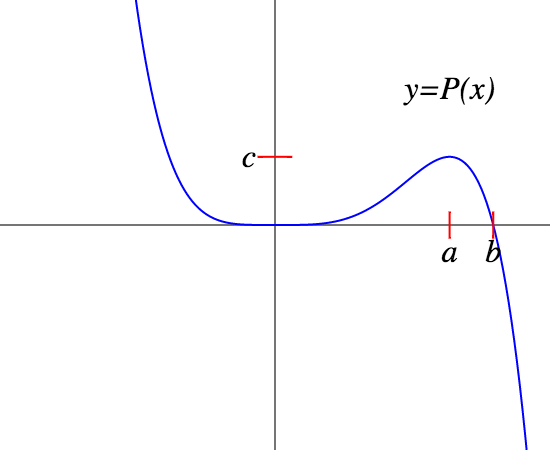
\includegraphics[scale=.38]{G18}
	\end{center}
\end{frame}

\begin{frame}[t]
	\frametitle{A sneaky function}

	Construct a function $f$ satisfying all the following properties:

	\begin{itemize}
		\item Domain $\displaystyle f = \mathbb{R}$

		\item $f$ is continuous

		\item $f'(0)=0$

		\item $f$ does not have a local extremum at $0$.

		\item There isn't an interval centered at $0$ on which $f$ is increasing.

		\item There isn't an interval centered at $0$ on which $f$ is decreasing.
	\end{itemize}
\end{frame}

\begin{frame}[t]
	\frametitle{Lake ripple}

	We drop a pebble into a lake. It produces a circular ripple. When the radius
	is $2$ meters and is increasing at a rate of $10cm/s$, at what rate is the area
	increasing?
\end{frame}

\begin{frame}[t]
	\frametitle{Sliding ladder}

	A ten-meter long ladder is leaning against a vertical wall and sliding. The top
	end of the ladder is 8 meters high and sliding down at a rate of 1 meter per second.
	At which rate is the bottom end sliding?
\end{frame}

\begin{frame}[t]
	\frametitle{Math party}

	The MAT137 TAs wanted to rent a disco ball for their upcoming party. However,
	since they are poor, they could only afford a flashlight. At the party, one TA
	is designated the ``human disco ball''. The TA stands in the center of the
	room pointing the flashlight horizontally and spins at 3 revolutions per
	second. (Yes, they are that fast. Ask your TA to demonstratel if you don't
	believe me!) The room is square with side length 8 meters. At which speed is the
	light from the flashlight moving across the wall when it is 3 meters away from
	a corner?
\end{frame}

\begin{frame}[t]
	\frametitle{Sleepy ants}

	Two ants are taking a nap. The first one is resting at the tip of the minute hand
	of a cuckoo clock, which is 25 cm long. The second one is resting at the tip of
	the hour hand, which is half the length. At what rate is the distance between the
	two ants changing at 3:30?
\end{frame}

\begin{frame}[t]
	\frametitle{The kite}

	Mary Poppins is flying a kite. The kite is 21 meters above the ground and it is
	being blown horizontally by the wind at 2 m/s. Mary's hands are 1 meter above
	the ground. Right now 30 meters of string are out. At what rate is the string
	being released from Mary's hands?
\end{frame}

\begin{frame}[t]
	\frametitle{Coffee}

	A coffee filter is shaped like an inverted cone. It has a radius at the top of
	$4cm$ and it is $6cm$ in height. Coffee flows out of at the bottom at a rate
	of $2cm^{3}/s$. If the filter begins completely filled, how fast is the coffee
	level decreasing after 30 seconds?
\end{frame}

\begin{frame}[t]
	\frametitle{The classic farmer problem}

	A farmer has $300m$ of fencing and wants to fence off a rectangular field and
	add an extra fence that divides the rectangular area in two equal parts down
	the middle. What is the largest area that the field can have?
\end{frame}

\begin{frame}[t]
	\frametitle{Distance}

	Find the point on the parabola $y^{2}=2x$ that is closest to the point $(1,4)$.
\end{frame}

\begin{frame}[t]
	\frametitle{A matter of perspective}

	A painting in an art gallery has height $h$ and is hung so that its lower edge
	is a distance $a$ above your eye. How far from the wall should you stand to get
	the best view?
\end{frame}

\begin{frame}[t]
	\frametitle{Airplane}

	The cost of fuel per hour for a certain airplane is proportional to the square
	of its speed and is \$1200 per hour for a speed of 600$km/h$. After every 5,000
	hours flown, the aircraft must undergo an \$8 million dollar safety inspection.
	What speed should the airplane fly at in order to achieve the lowest cost per
	kilometre?
\end{frame}

\begin{frame}[t]
	\frametitle{Fire}

	You hear a scream. You turn around and you see Alfonso is on fire. Literally! Luckily,
	you are next to a straight river. Alfonso is 10 meters away from the river and
	you are 5 meters away from the point $P$ on the river closest to Alfonso. You
	are carrying an empty bucket. You can run twice as fast with an empty bucket as
	you can run with a full bucket. How far from the point P should you fill your
	bucket in order to get to Alfonso with a bucket full of water as fast as
	possible?

	% Warning!  This problem is a trap.  If you model it carelessly, it has  a critical point but it is outside the domain.
\end{frame}

\begin{frame}[t]
	\frametitle{Dominion}

	Dominion is a board game where, among other things, players buy cards worth
	victory points. The player with the most victory points wins.

	It is your last turn and you can only buy ``duchies'' and ``dukes''. A duchy
	is worth 3 victory points. A duke is worth as many victory points as duchies you
	have. Each duchy costs 3 coins, and each duke costs 3 coins. You have not
	bough any duke or duchy yet.

	If you have $N$ coins, how many dukes and how many duchies should you buy?
\end{frame}

\begin{frame}[t]
	\frametitle{Limits from graphs}

	Compute:

	\begin{multicols}{2}
		\begin{enumerate}
			\item $\displaystyle \lim_{x\to 0 }\frac{H(x)}{H(2+3x) - 1}$

			\item $\displaystyle \lim_{x \to 2}\frac{F^{-1}(x)}{x-2}$
		\end{enumerate}
	\end{multicols}

	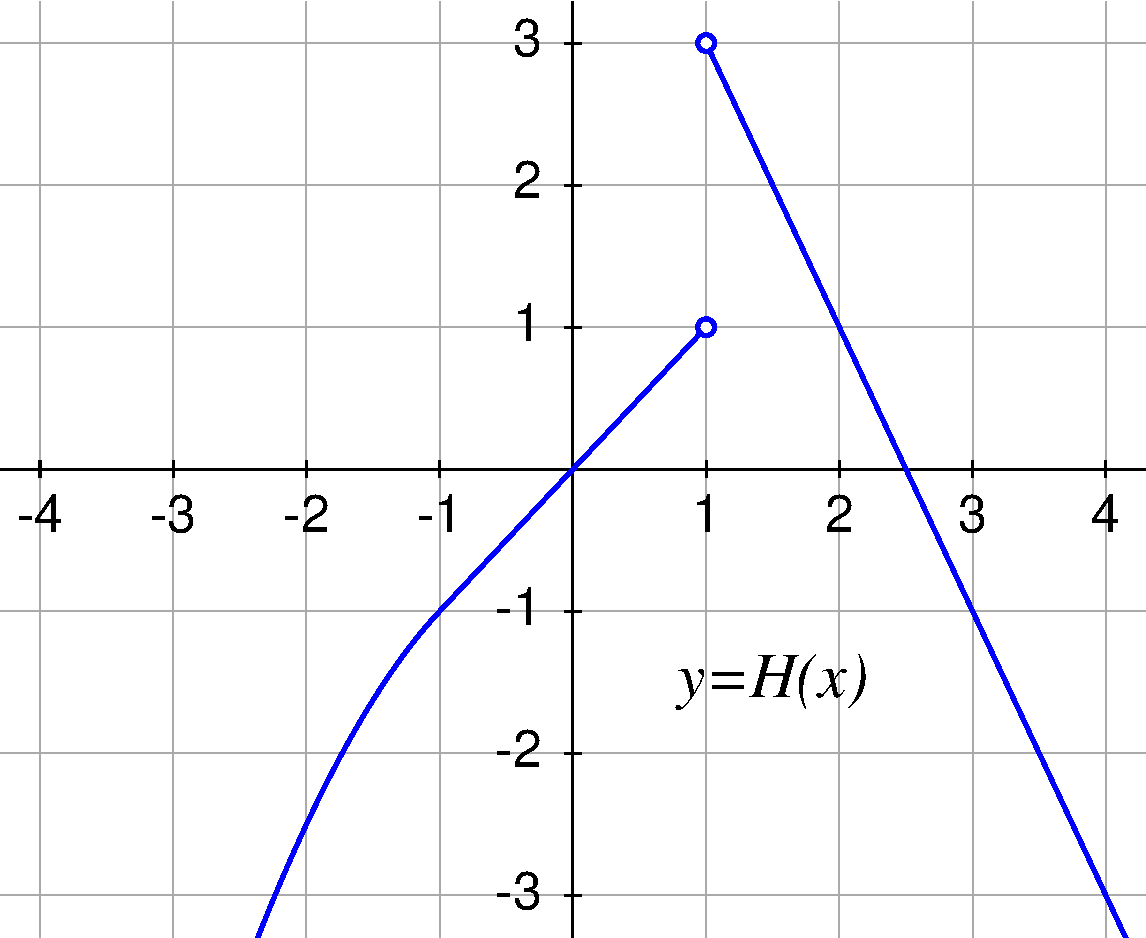
\includegraphics[scale=.29]{G14}
	\hfill
	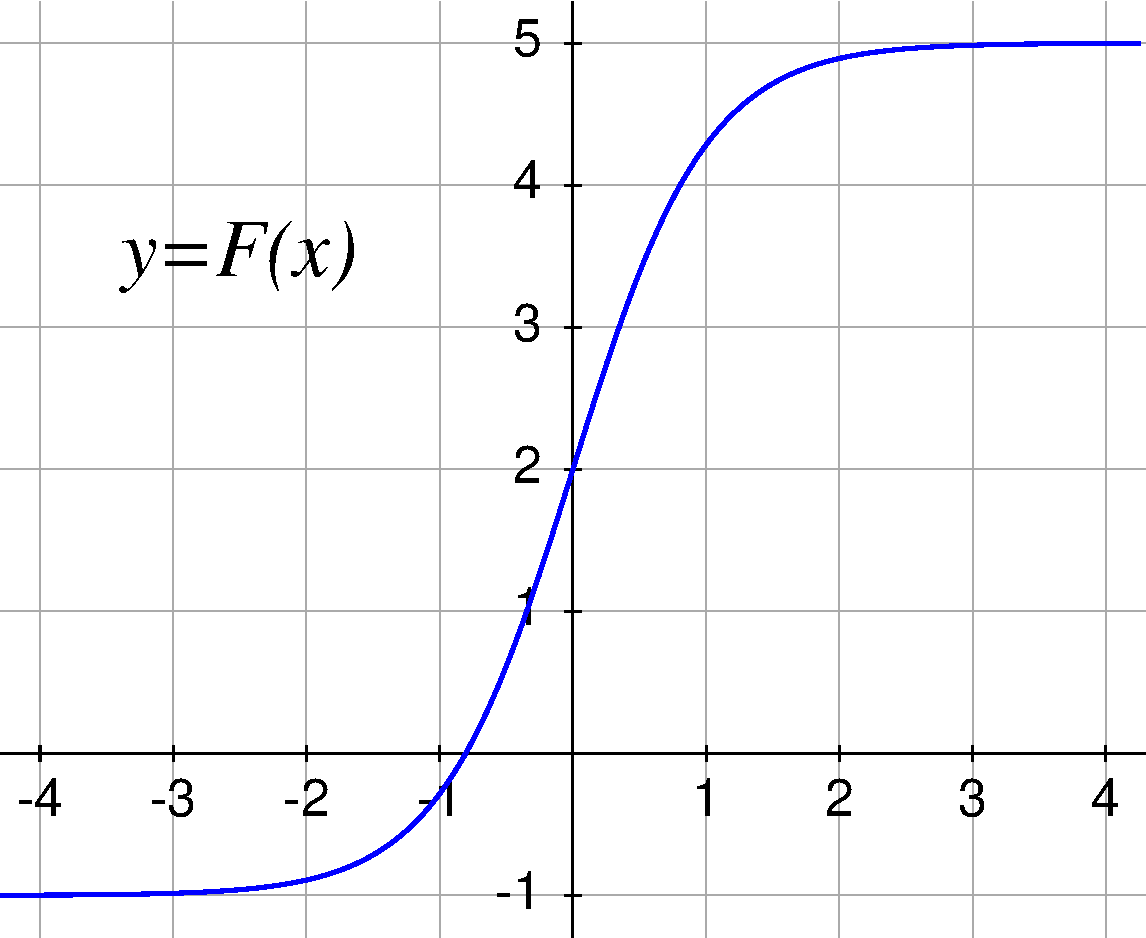
\includegraphics[scale=.29]{G15}
\end{frame}

\begin{frame}[t]
	\frametitle{Polynomial vs Exponential}

	\begin{enumerate}
		\item Use L'H\^{o}pital Rule to compute
			\[
				\lim_{x \to \infty}\frac{x^{7}+ 5x^{3}+2}{e^{x}}
			\]

			\
		% \pause

		\item Make a conjecture for the value of
			\[
				\lim_{x \to \infty}\frac{x^{N}}{e^{x}}
			\]
			where $N$ is a positive integer. Prove it by induction.
	\end{enumerate}
\end{frame}

\begin{frame}[t]
	\frametitle{Computations}

	Calculate:

	\begin{multicols}{2}
		\begin{enumerate}
			\item $\displaystyle \lim_{x \to 2}\frac{x^{2}+2x - 6}{x^{2}+3x-10}$

			\item $\displaystyle \lim_{x \to 0}\frac{e^{2x^2}- \cos x}{x \sin x}$

			\item $\displaystyle \lim_{x \to \infty}x^{3}e^{-x}$

			\item $\displaystyle \lim_{x \to \infty}\frac{e^{x}+ e^{-x}}{e^{x}- e^{-x}}$

			\item $\displaystyle \lim_{x \to 0}\, x \sin \frac{2}{x}$

			\item $\displaystyle \lim_{x \to \infty}x \sin \frac{2}{x}$

			\item $\displaystyle \lim_{x \to \infty}x \cos \frac{2}{x}$

			\item $\displaystyle \lim_{x \to 1}\left[ \left( \ln x \right) \tan \frac{\pi
				x}{2}\right]$
		\end{enumerate}
	\end{multicols}
\end{frame}

\begin{frame}[t]
	\frametitle{Infinity minus infinity}

	Calculate:

	\begin{enumerate}
		\item $\displaystyle \lim_{x \to 0}\left[ \frac{\csc x}{x}- \frac{\cot x}{x}\right
			]$

			\

		\item $\displaystyle \lim_{x \to \infty}\left[ \ln (x+2) - \ln(3x+4) \right]$

			\

		\item $\displaystyle \lim_{x \to 1}\left[ \frac{2}{x^{2}-1}- \frac{1}{x-1}\right
			]$

		\item $\displaystyle \lim_{x \to - \infty}\left[ \sqrt{x^{2}+3x}- \sqrt{x^{2}-3x}
			\right]$
	\end{enumerate}
\end{frame}

\begin{frame}[t]
	\frametitle{Exponential indeterminate forms}

	Calculate:

	\begin{enumerate}
		\item $\displaystyle \lim_{x \to 0}\left[ 1 + 2 \sin(3x) \right]^{4 \cot (5x)}$

		\item $\displaystyle \lim_{x \to \infty }\left( \frac{x+2}{x-2}\right)^{3x}$

		\item $\displaystyle \lim_{x \to 0^+}x^{x}$

		\item $\displaystyle \lim_{x \to {\frac{\pi}{2}}^{-}}\left( \tan x \right)^{\cos
			x}$

		\item $\displaystyle \lim_{x \to 0}\left( \frac{\sin x}{x}\right)^{1 /x^2}$
	\end{enumerate}
\end{frame}

\begin{frame}[t]
	\frametitle{Backwards L'H\^{o}pital}

	Construct a polynomial $P$ such that
	\[
		\lim_{x \to 1}\; \frac{P(x)}{e^{x}- e \cdot x}\; = \; \frac{1}{e}
	\]
\end{frame}

\begin{frame}[t]
	\fontsize{13}{13}\selectfont
	\frametitle{Come to the dark side}

	Help us write a difficult question for Test 3! We will ask you to compute a
	limit like this
	\[
		\lim_{x \to 0}\frac{e^{x}+ e^{-x}- 2 \cos x + bx^{N}}{x^{6}}
	\]
	where $b$ is a real number and $N$ is a natural number that we have not chosen
	yet.

	We do not want the answer to be $0$ or $\infty$ or $-\infty$ or ``DNE",
	because you could guess that randomly.

	What values of $b$ and $N$ should we choose? What will the value of the limit be?
\end{frame}

\begin{frame}[t]
	\frametitle{Indeterminate?}

	Which of the following are indeterminate forms for limits? \\ If any of them isn't,
	then what is the value of such limit?

	\begin{multicols}{4}
		\begin{enumerate}
			\setlength{\itemsep}{1em}

			\item $\displaystyle \frac{0}{0}$

			\item $\displaystyle \frac{0}{\infty}$

			\item $\displaystyle \frac{0}{1}$

			\item $\displaystyle \frac{\infty}{0}$

			\item $\displaystyle \frac{\infty}{\infty}$

			\item $\displaystyle \frac{1}{\infty}$

			\item $\displaystyle 0 \cdot \infty$ \phantom{$\displaystyle \frac{1}{1}$}

			\item $\displaystyle \infty \cdot \infty$ \phantom{$\displaystyle \frac{1}{1}$}

			\item $\displaystyle \sqrt{\infty}$

			\item $\displaystyle \infty - \infty$

			\item $\displaystyle 1^{\infty}$

			\item $\displaystyle 1^{-\infty}$

			\item $\displaystyle 0^{0}$

			\item $\displaystyle 0^{\infty}$

			\item $\displaystyle 0^{-\infty}$

			\item $\displaystyle \infty^{0}$

			\item $\displaystyle \infty^{\infty}$

			\item $\displaystyle \infty^{-\infty}$
		\end{enumerate}
	\end{multicols}
\end{frame}

\begin{frame}[t]
	\fontsize{13}{13}\selectfont
	\frametitle{Proving something is an indeterminate form}

	\begin{enumerate}
		\item Prove that $\displaystyle \forall c \in \mathbb{R}$,
			$\displaystyle \exists a \in \mathbb{R}$ and functions $f$ and $g$ such
			that
			\[
				\lim_{x \to a}f(x) = 0, \quad \lim_{x \to a}g(x) =0, \quad \lim_{x \to a}
				\frac{f(x)}{g(x)}= c
			\]

			This is how you show that $\displaystyle \frac{0}{0}$ is an indeterminate form.

			\
		% \pause

		\item Prove the same way that $\displaystyle \frac{\infty}{\infty}$,
			$\displaystyle 0 \cdot \infty$, and $\displaystyle \infty - \infty$ are also
			indeterminate forms.

			\
		% \pause

		\item Prove that $\displaystyle 1^{\infty}$, $\displaystyle 0^{0}$, and $\displaystyle
			\infty^{0}$ are indeterminate forms.

			(You will only get $c \geq 0$ this time)
	\end{enumerate}
\end{frame}

\begin{frame}[t]
	\frametitle{Find the coordinates of $P$ and $Q$}
	\vspace{-.5cm}
	\[
		g(x) = x^{4}- 6x^{2}+ 9
	\]

	\begin{center}
		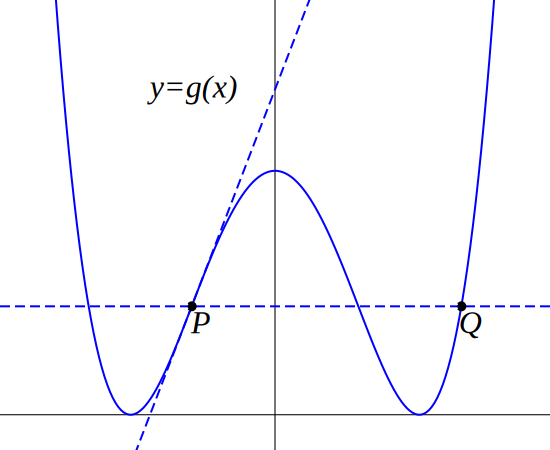
\includegraphics[scale=.4]{G16}
	\end{center}
\end{frame}

\begin{frame}[t]
	\frametitle{Find the coordinates of $P$ }

	\[
		f(x) = 3x+4 + \frac{2x-10}{x^{2}}
	\]

	\begin{center}
		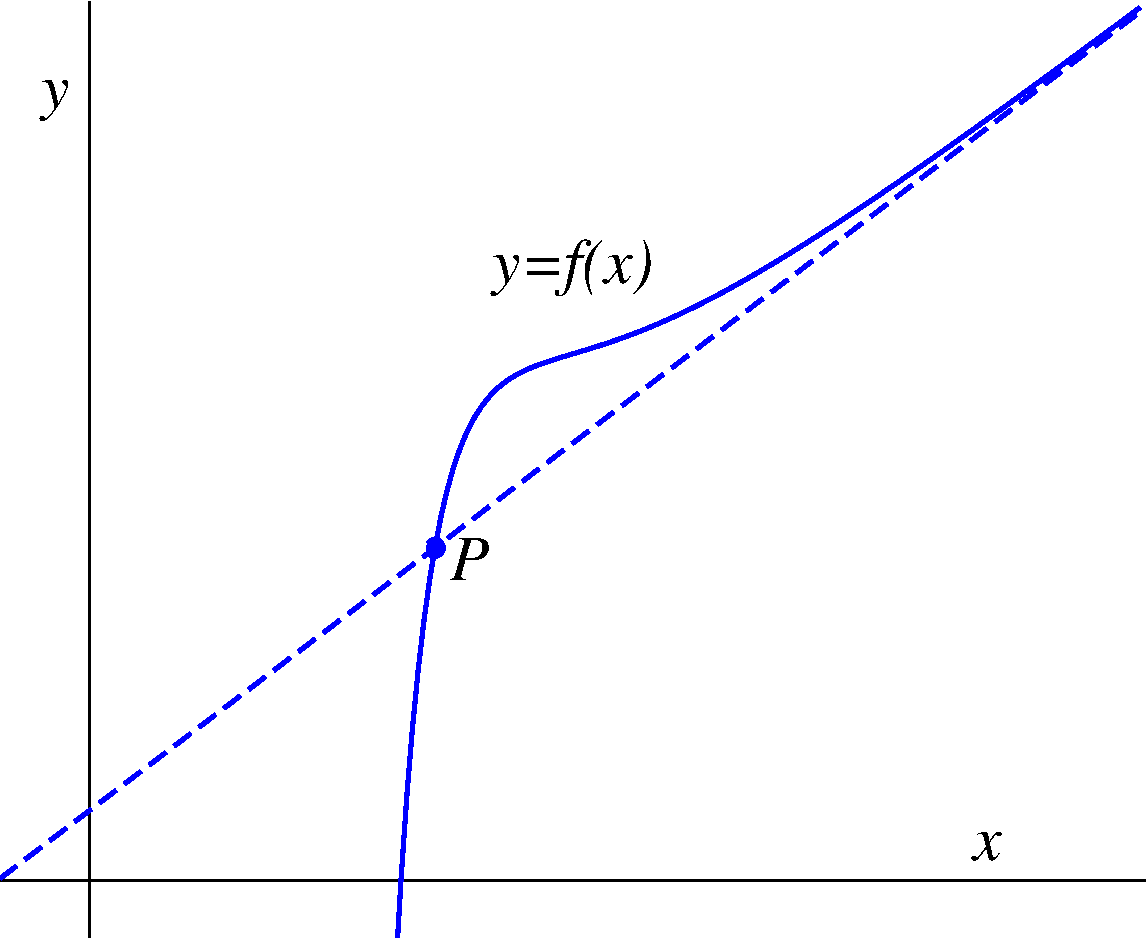
\includegraphics[scale=0.4]{G17}
	\end{center}
\end{frame}

\begin{frame}[t]
	\fontsize{13}{13}\selectfont
	\frametitle{True or False -- Concavity and inflection points}

	Let $f$ be a {{differentiable}} function with domain $\mathbb{R}$. \\ Let
	$c \in \mathbb{R}$. Let $I$ be an interval. Which implications are true?

	\begin{enumerate}
		\item IF {\color{red} $f$ is concave up on $I$}, \quad THEN
			{\color{blue} $\forall x \in I$, $f''(x) >0$}.

		\item IF {\color{blue} $\forall x \in I$, $f''(x) >0$}, \quad THEN
			{\color{red} $f$ is concave up on $I$}.

		\item IF {\color{red} $f$ is concave up on $I$} \quad THEN {\color{verde} $f'$ is increasing on $I$}.

		\item IF {\color{verde} $f'$ is increasing on $I$}, \quad THEN
			{\color{red} $f$ is concave up on $I$}.

		\item IF {\color{rosa} $f$ has an I.P.\ at $c$}, \quad THEN
			{\color{naranja} $f''(c)=0$}.

		\item IF {\color{naranja} $f''(c)=0$}, \quad THEN
			{\color{rosa} $f$ has an I.P.\ at $c$}.

		\item IF {\color{rosa} $f$ has an I.P. at $c$}, \quad THEN
			{\color{violet} $f'$ has a local extremum at $c$}

		\item IF {\color{violet} $f'$ has a local extremum at $c$}, \quad THEN
			{\color{rosa} $f$ has an I.P.\ at $c$}.
	\end{enumerate}
	\begin{center}
		I.P.\  = ``inflection point"
	\end{center}
\end{frame}

\begin{frame}[t]
	\fontsize{13}{13}\selectfont
	\frametitle{``Secant segments are above the graph"}

	Let $f$ be a function defined on an interval $I$.\\ In Video 6.13 you learned that
	an alternative to our definition of ``$f$ is concave up on $I$" is ``the
	secant segments stay above the graph".

	\begin{center}
		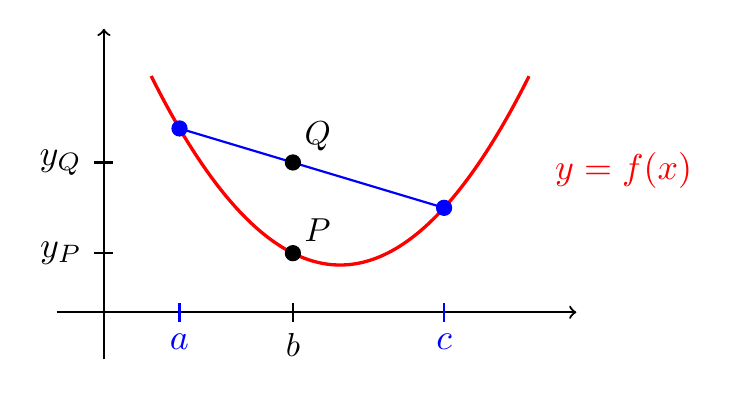
\begin{tikzpicture}[scale=1.2]
			\draw[thick, ->] (-0.5,0) -- (5,0);
			\draw[thick, ->] (0,-0.5) -- (0,3);
			\draw[domain=0.5:4.5, smooth, variable=\x, samples={200}, red, very thick]
				plot
				({\x}, {(\x-2.5)*(\x-2.5)/2 + .5});
			\node[red, scale=1.3] at (5.5,1.5) {$\displaystyle y=f(x)$};
			\draw[blue, fill] (.8,1.945) circle[radius=0.08];
			\draw[blue, fill] (3.6,1.105) circle[radius=0.08];
			\draw[thick, blue] (.8,-.1) to (.8,.1);
			\node[below, blue, scale=1.3] at (.8,-.1) {$a$};
			\draw[thick, blue] (3.6,-.1) to (3.6,.1);
			\node[below, blue, scale=1.3] at (3.6,-.1) {$c$};
			\draw[blue, thick] (.8,1.945) -- (3.6,1.105);
			\draw[thick] (2,-.1) to (2,.1);
			\node[below, black, scale=1.2] at (2,-.1) {$b$};
			\draw[black, fill] (2,0.625) circle[radius=0.08];
			\node[above right, black, scale=1.2] at (2,0.625) {$P$};
			\draw[black, fill] (2,1.585) circle[radius=0.08];
			\node[above right, black, scale=1.2] at (2,1.585) {$Q$};
			\draw[thick] (-.1,0.625) to (.1,.625);
			\node[left, black, scale=1.3] at (-.1,0.625) {$y_{P}$};
			\draw[thick] (-.1,1.585) to (.1,1.585);
			\node[left, black, scale=1.3] at (-.1,1.585) {$y_{Q}$};
		\end{tikzpicture}
	\end{center}

	Rewrite this as a precise mathematical statement of the form
	\[
		``\forall a,b,c \in I, \quad a<b<c \; \implies \; \boxed{\text{an inequality involving $f$, $a$, $b$, $c$}}
		"
	\]
\end{frame}

\begin{frame}[t]
	\frametitle{A polynomial from 3 points}

	Construct a polynomial that satisfies the following three properties at once:
	\begin{enumerate}
		\item It has an inflection point at $x=2$

		\item It has a a local extremum at $x=1$

		\item It has $y$-intercept at $y=1$.
	\end{enumerate}
\end{frame}

\begin{frame}[t]
	\frametitle{Monotonicity and concavity}

	Let $\displaystyle f(x) = x e^{-x^2/2}$.

	\begin{enumerate}
		\item Find the intervals where $f$ is increasing or decreasing, and its
			local extrema.

		\item Find the intervals where $f$ is concave up or concave down, and its
			inflection points.

		\item Calculate $\displaystyle \lim_{x \to \infty}f(x)$ and $\displaystyle \lim
			_{x \to - \infty}f(x)$.

		\item Using this information, sketch the graph of $f$.
	\end{enumerate}
\end{frame}

\begin{frame}[t]
	\frametitle{Fractional exponents}

	Let $\displaystyle h(x) = \frac{x^{2/3}}{(x-1)^{2/3}}$. Its first two derviatives
	are
	\begin{equation*}
		h'(x) = \frac{-2}{3x^{1/3}(x-1)^{5/3}}\; \quad \quad h''(x) = \frac{2(6x-1)}{9x^{4/3}(x-1)^{8/3}}
	\end{equation*}

	\begin{enumerate}
		\item Find all asymptotes of $h$

		\item Study the monotonicity of $h$ and local extrema

		\item Study the concavity of $h$ and inflection points

		\item With this information, sketch the graph of $h$
	\end{enumerate}
\end{frame}

\begin{frame}[t]
	\frametitle{Hyperbolic tangent}

	The function $\tanh$, defined by
	\[
		\tanh x = \frac{e^{x}- e^{-x}}{e^{x}+ e^{-x}},
	\]
	is called the ``hyperbolic tangent".
	\begin{enumerate}
		\item Find its two asymptotes

		\item Study its monotonicity

		\item Study its concavity

		\item With this information, sketch its graph.
	\end{enumerate}
\end{frame}

\begin{frame}[t]
	\frametitle{A very hard function to graph}

	The function $\displaystyle G(x) = x e^{1/x}$ is deceiving. To help you out:
	\[
		G'(x) = \frac{x-1}{x}e^{1/x}, \quad \quad G''(x) = \frac{e^{1/x}}{x^{3}}
	\]

	\begin{enumerate}
		\item Carefully study the behaviour as $x \to \pm \infty$. \\ You should
			find an asymptote, but it is not easy.

		\item Carefully study the behaviour as $x \to 0^{+}$ and $x\to 0^{-}$. The
			two are very different.

		\item Use $G'$ to study monotonocity.

		\item Use $G''$ to study concavity.

		\item Sketch the graph of $G$.
	\end{enumerate}
\end{frame}

\begin{frame}[t]
	\frametitle{Backwards graphing }

	$R$ is a rational function (a quotient of polynomials). \\ Find its equation.
	\begin{center}
		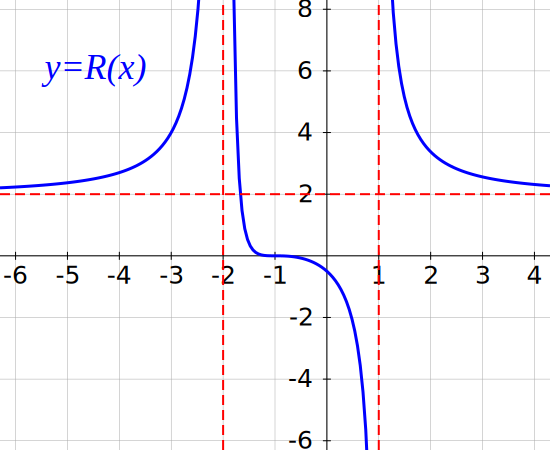
\includegraphics[scale=.4]{G19}
	\end{center}
\end{frame}

\begin{frame}[t]
	\frametitle{Unexpected asymptotes}

	Find the two asymptotes of the function
	\[
		F(x) = x + \sqrt{x^{2}+2x+ 2}
	\]

	\emph{Hint:} The behaviour as $x \to \infty$ is very different from
	$x \to - \infty$.

	\ \hfill \href{https://www.desmos.com/calculator/kffnbl6pnc}{\beamergotobutton{graph}}
\end{frame}

\begin{frame}[t]
	\frametitle{Unusual examples}

	Construct three functions $f$, $g$, and $h$.

	\begin{enumerate}
		\item $f$ has domain at least $(0,\infty)$, is continuous, is always concave
			up, and satisfies $\displaystyle \lim_{x \to \infty}f(x) = - \infty$

		\item $g$ has domain $\mathbb{R}$, is continuous, has a local minimum at $x=0$,
			and has an inflection point also at $x=0$.

		\item $h$ has domain $\mathbb{R}$, is differentiable, is strictly increasing.
			In addition, $h'$ is periodic with period $2$, and $h'$ is not constant.
	\end{enumerate}
\end{frame}

\begin{frame}[t]
	\frametitle{Warm-up: sums}

	Compute

	\begin{enumerate}
		\item $\displaystyle \sum_{i=2}^{4}(2i+1)$
			\vfill

		\item $\displaystyle \sum_{i=2}^{4}2i + 1$
			\vfill

		\item $\displaystyle \sum_{j=2}^{4}(2i + 1)$
			\vfill
	\end{enumerate}
\end{frame}

\begin{frame}[t]
	\fontsize{13}{13}\selectfont
	\frametitle{Write these sums with $\Sigma$ notation}

	\begin{enumerate}
		\item $\displaystyle 1^{5}+ 2^{5}+ 3^{5}+ 4^{5}+ \ldots + 100^{5}$
			\vfill

		\item $\displaystyle \frac{2}{4^{2}}+ \frac{2}{5^{2}}+ \frac{2}{6^{2}}+ \frac{2}{7^{2}}
			+ \ldots + \frac{2}{N^{2}}$
			\vfill

		\item $\displaystyle \cos 0 - \cos 1 + \cos 2 - \cos 3 + %\cos 4 -
			\ldots \pm \cos (N+1)$
			\vfill

		\item $\displaystyle \frac{1}{0!}+ \frac{1}{2!}+ \frac{1}{4!}+ \frac{1}{6!}+
			\ldots + \frac{1}{(2N)!}$
			\vfill

		\item $\displaystyle \frac{1}{1!}- \frac{1}{3!}+ \frac{1}{5!}- \frac{1}{7!}+
			\ldots + \frac{1}{81!}$
			\vfill

		\item $\displaystyle \frac{2x^{3}}{ 4!}+ \frac{3x^{4}}{5!}+ \frac{4x^{5}}{6!}
			+ \ldots + \frac{999x^{1000}}{1001!}$
	\end{enumerate}
\end{frame}

\begin{frame}[t]
	\fontsize{13}{13}\selectfont
	\frametitle{Re-writing sums}

	\begin{enumerate}
		\item $\displaystyle \sum_{i=1}^{100}\tan i \, - \, \sum_{i=1}^{50}\tan i \;
			= \; \sum_{\boxed{\phantom{???}}}^{\boxed{\phantom{???}}}\boxed{\phantom{?????^f_p}}$
			\vfill

		\item $\displaystyle \sum_{i=1}^{N}(2i-1)^{5}\; = \; \sum_{i=0}^{N-1}\boxed{\phantom{?????^f_p}}$
			\vfill

		\item $\displaystyle \left[ \sum_{k=1}^{N}x^{k}\right] \, + \, \left[ \sum_{k=0}
			^{N}k \; x^{k+1}\right] \; = \; \left[ \sum_{k=\boxed{\phantom{???}}}^{\boxed{\phantom{???}}}
			\!\!\boxed{\phantom{???}}\,x^{k}\right] \, + \, \boxed{\phantom{???}}$
			\vfill
	\end{enumerate}

	\emph{Hint:} Write out the sums on the left hand side first, simplify if
	possible, then write them back into sigma notation.
\end{frame}

\begin{frame}[t]
	\frametitle{Telescopic sum}

	\begin{itemize}
		\item Calculate the exact value of
			\[
				\sum_{i=1}^{137}\left[ \frac{1}{i}- \frac{1}{i+1}\right]
			\]
			\emph{Hint:} Write down the first few terms.

		% \pause

		\item Calculate the exact value of
			\[
				\sum_{i=1}^{10,000}\frac{1}{i(i+1)}
			\]
	\end{itemize}
\end{frame}

\begin{frame}[t]
	\frametitle{Double sums}

	Compute:
	\begin{multicols}{3}
		\begin{enumerate}
			\item $\displaystyle \sum_{i=1}^{N}\sum_{k=1}^{N}1$

			\item $\displaystyle \sum_{i=1}^{N}\sum_{k=1}^{i}1$

			\item $\displaystyle \sum_{i=1}^{N}\sum_{k=1}^{i}i$

			\item $\displaystyle \sum_{i=1}^{N}\sum_{k=1}^{i}k$

			\item $\displaystyle \sum_{i=1}^{N}\sum_{k=1}^{i}(ik)$
		\end{enumerate}
	\end{multicols}

	\vfill

	{\fontsize{10}{10}\selectfont Useful formulas: \begin{align*}&\sum_{j=1}^{N}j = \frac{N(N+1)}{2},&&\sum_{j=1}^{N}j^{2}= \frac{N(N+1)(2N+1)}{6},&&\sum_{j=1}^{N}j^{3}= \frac{N^{2}(N+1)^{2}}{4}\end{align*} }
\end{frame}

\begin{frame}[t]
	\fontsize{13}{13}\selectfont
	\frametitle{Harmonic sums}

	We define the $N$-th Harmonic term as the sum
	\[
		H_{N}\; = \; 1 + \frac{1}{2}+ \frac{1}{3}+ \ldots + \frac{1}{N}\; = \; \sum_{i=1}
		^{N}\frac{1}{i}.
	\]

	Write the following sums in terms of harmonic terms.

	\begin{multicols}{2}
		\begin{enumerate}
			\item $\displaystyle \sum_{i=k}^{N}\; \frac{1}{i}$

			\item $\displaystyle \frac{1}{2}+ \frac{1}{4}+ \frac{1}{6}+ \ldots + \frac{1}{2N}$

			\item $\displaystyle \sum_{i=1}^{N}\; \frac{1}{2i-1}$

			\item $\displaystyle \sum_{i=1}^{2N}\; \frac{(-1)^{i+1}}{i}$
		\end{enumerate}
	\end{multicols}
\end{frame}

\begin{frame}[t]
	\fontsize{13}{13}\selectfont
	\frametitle{Fubini-Tonelli}

	\begin{itemize}
		\item $A_{i,k}$ is a function of 2 variables. \; For example, $\displaystyle
			A_{i,k}= \frac{i}{k+i^{2}}$.

		\item Decide what to write instead of each ``\boxed{\mbox{{\color{red} ?}}}''
			so that the following identity is true:
	\end{itemize}

	{\fontsize{20}{20}\selectfont \begin{equation*}\sum_{i=1}^{N}\; \sum_{k=1}^{i}A_{i, k}= \sum_{k = \boxed{{\color{red} ?}}}^{\boxed{{\color{red} ?}}}\; \sum_{i=\boxed{{\color{red} ?}}}^{\boxed{{\color{red} ?}}}A_{i,k}\end{equation*} }
\end{frame}

\begin{frame}[t]
	\fontsize{13}{13}\selectfont
	\frametitle{Warm up: suprema and infima}

	Find the supremum, infimum, maximum, and minimum of the following sets (if they
	exist):

	\begin{enumerate}
		\vfill

		\item $\displaystyle A = [-1,5)$
			\vfill

		\item $\displaystyle B = (-\infty,6] \cup (8, 9)$
			\vfill

		\item $\displaystyle C = \{ 2, 3, 4\}$
			\vfill

		\item $\displaystyle D = \left\{ \frac{1}{n}\; : \; n \in \mathbb{Z}, \, n >0
			\right\}$
			\vfill

		\item $\displaystyle E = \left\{ \frac{(-1)^{n}}{n}\; : \; n \in \mathbb{Z},
			\, n >0 \right\}$
			\vfill

		\item $\displaystyle F = \left\{ 2^{n}\; : \; n \in \mathbb{Z}\right\}$
			\vfill
	\end{enumerate}
\end{frame}

\begin{frame}[t]
	\fontsize{13}{13}\selectfont
	\frametitle{Suprema from a graph}

	Calculate, for the function $g$ on the interval $[0.5, 1.5]$:
	\begin{enumerate}
		\begin{multicols}{4}
			\item supremum \item infimum \item maximum \item minimum
		\end{multicols}
	\end{enumerate}

	\begin{center}
		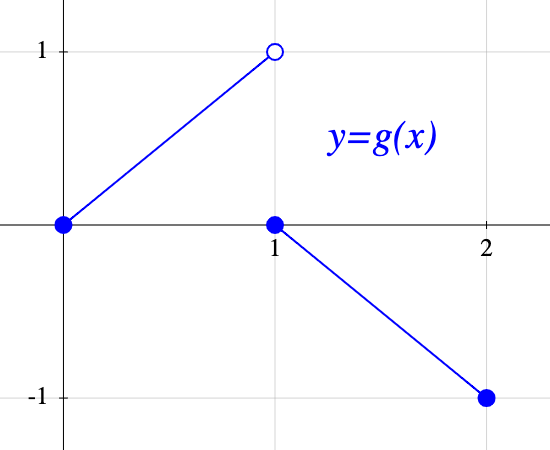
\includegraphics[scale=.35]{G20}
	\end{center}
\end{frame}

\begin{frame}[t]
	\frametitle{Trig suprema}

	Let $f(x) = \sin x$. \\ Find four open intervals $I_{1}$, $I_{2}$, $I_{3}$,
	$I_{4}$ such that

	\begin{enumerate}
		\item $f$ has a supremum and an infimum on $I_{1}$.

		\item $f$ has a supremum and no infimum on $I_{2}$.

		\item $f$ has a maximum and a minimum on $I_{3}$.

		\item $f$ has a maximum and no minimum on $I_{4}$.
	\end{enumerate}
\end{frame}

\begin{frame}[t]
	\frametitle{Empty set}

	\begin{enumerate}
		\item Does $\emptyset$ have an upper bound ?

		\item Does $\emptyset$ have a supremum?

		\item Does $\emptyset$ have a maximum?

		\item Is $\emptyset$ bounded above?
	\end{enumerate}
\end{frame}

\begin{frame}[t]
	\fontsize{13}{13}\selectfont
	\frametitle{Equivalent definitions of supremum}

	{\bfseries Assume $S$ is an upper bound of the set $A$.} \\ Which of the following
	is equivalent to ``$S$ is the supremum of $A$"?
	\vspace{.2cm}
	\begin{enumerate}
		\item If $R$ is an upper bound of $A$, \, then $S \leq R$.
			\vspace{.2cm}

		\item $\displaystyle \forall R \geq S$, \, $R$ is an upper bound of $A$.

		\item $\displaystyle \forall R \leq S$, \, $R$ is not an upper bound of $A$.

		\item $\displaystyle \forall R < S$, \, $R$ is not an upper bound of $A$.
			\vspace{.2cm}

		\item $\displaystyle \forall R < S$, \, $\displaystyle \exists x \in A$ \;
			such that \; $\displaystyle R < x$.

		\item $\displaystyle \forall R < S$, \, $\displaystyle \exists x \in A$ \;
			such that \; $\displaystyle R \leq x$.

		\item $\displaystyle \forall R < S$, \, $\displaystyle \exists x \in A$ \;
			such that \; $\displaystyle R < x \leq S$.

		\item $\displaystyle \forall R < S$, \, $\displaystyle \exists x \in A$ \;
			such that \; $\displaystyle R < x < S$.
			\vspace{.2cm}

		\item $\displaystyle \forall \varepsilon>0$, \; \,
			$\displaystyle \exists x \in A$ \; such that \;
			$\displaystyle S - \varepsilon < x$.

		\item $\displaystyle \forall \varepsilon>0$, \; \,
			$\displaystyle \exists x \in A$ \; such that \;
			$\displaystyle S - \varepsilon < x \leq S$.
	\end{enumerate}
\end{frame}

\begin{frame}[t]
	\fontsize{13}{13}\selectfont
	\frametitle{Fix these FALSE statements}

	\begin{enumerate}
		\item Let $f$ and $g$ be bounded functions on $[a,b]$. Then
			\[
				\; \substack{\text{ $\sup$ of $(f+g)$} \\ \text{on $[a,b]$} }\; \quad = \quad
				\; \substack{\text{ $\sup$ of $f$} \\ \text{on $[a,b]$} }\; \quad + \quad
				\; \substack{\text{ $\sup$ of $g$} \\ \text{on $[a,b]$} }\;
			\]

			\vfill

		\item Let $a < b < c$. Let $f$ be a bounded function on $[a,c]$. Then
			\[
				\; \substack{\text{ $\sup$ of $f$} \\ \text{on $[a,c]$} }\; \quad = \quad
				\; \substack{\text{ $\sup$ of $f$} \\ \text{on $[a,b]$} }\; \quad + \quad
				\; \substack{\text{ $\sup$ of $f$} \\ \text{on $[b,c]$} }\;
			\]

			\vfill

		\item Let $f$ be a bounded function on $[a,b]$. Let $c \in \mathbb{R}$. Then:
			\[
				\; \substack{\text{ $\sup$ of $(cf)$} \\ \text{on $[a,b]$} }\; \quad = \quad
				c \; \left( \; \substack{\text{ $\sup$ of $f$} \\ \text{on $[a,b]$} }\; \right
				)
			\]
	\end{enumerate}
\end{frame}

\begin{frame}[t]
	\fontsize{12}{12}\selectfont
	\frametitle{True or False - Suprema and infima}

	Let $A, B, C \subseteq \mathbb{R}$. Assume $C \subseteq A$. Which statements are
	true?
	\vspace{.1cm}

	If possible, fix the false statements
	\vspace{.2cm}
	\begin{enumerate}
		\item IF \;$A$ is bounded above, \; THEN \;$C$ is bounded above.

		\item IF \;$C$ is bounded below, \; THEN \;$A$ is bounded below.
			\vspace{.2cm}

		\item IF \;$A$ and $C$ are bounded above, \; THEN \;$\sup C \leq \sup A$.

		\item IF \;$A$ and $C$ are bounded below, \; THEN \;$\inf C \leq \inf A$.
			\vspace{.2cm}

		\item IF \;$A$ and $B$ are bounded, \;$\sup B \leq \sup A$, \;and \;$\inf A \leq
			\inf B$,
			\vspace{.1cm}

			THEN \;$B \subseteq A$.
			\vspace{.2cm}

		\item IF \;$A$ and $B$ are bounded above,
			\vspace{.1cm}

			THEN \;$\displaystyle \sup (A \cup B) =\max \{ \sup A, \sup B \}$.
			\vspace{.2cm}

		\item IF \;$A$ and $B$ are bounded above,
			\vspace{.1cm}

			THEN \;$\displaystyle \sup (A \cap B) =\min \{ \sup A, \sup B \}$.
	\end{enumerate}
\end{frame}

\begin{frame}[t]
	\frametitle{Warm up: partitions}

	Which ones are partitions of $[0,2]$?

	\begin{enumerate}
		\item $\displaystyle [0,2]$

		\item $\displaystyle \{0.5, \,1, \,1.5\}$

		\item $\displaystyle \{0,\,2\}$

		\item $\displaystyle \{1,\,2\}$

		\item $\displaystyle \{0, \,e, \,2 \}$

		\item $\displaystyle \{0, \,1.5, \,1.6, \,1.7, \,1.8, \,1.9, \,2\}$

		\item $\displaystyle \left\{ \frac{n}{n+1}\; : \; n \in \mathbb{N}\right\} \cup
			\{ 2 \}$
	\end{enumerate}
\end{frame}

\begin{frame}[t]
	\fontsize{13}{13}\selectfont
	\frametitle{Partitions of different intervals}

	Let $a<b<c$. Which of these statements are true?

	If any are false, fix them.
	\vspace{.1cm}
	\begin{enumerate}
		\item IF $P$ and $Q$ are partitions of $[a,b]$,
			\vspace{.1cm}

			THEN $P \cup Q$ is a partition of $[a,b]$.
			\vspace{.1cm}

		\item IF $P$ and $Q$ are partitions of $[a,b]$,
			\vspace{.1cm}

			THEN $P \cap Q$ is a partition of $[a,b]$.
			\vspace{.1cm}

		\item IF $P$ is a partition of $[a,b]$ and $Q$ is a partition of $[b,c]$
			\vspace{.1cm}

			THEN $P \cup Q$ is a partition of $[a,c]$
			\vspace{.1cm}

		\item IF $P$ is a partition of $[a,c]$,
			\vspace{.1cm}

			THEN $P \cap [a,b]$ is a partition of $[a,b]$
	\end{enumerate}
\end{frame}

\begin{frame}[t]
	\frametitle{Warm up: lower and upper sums}

	Let $\displaystyle f(x) = \sin x$.

	Consider the partition $\displaystyle P= \{0, 1, 3\}$ of the interval
	$\displaystyle [0,3]$.

	Calculate $\displaystyle L_{P}(f)$ and $\displaystyle U_{P}(f)$.
\end{frame}

\begin{frame}[t]
	\fontsize{13}{13}\selectfont
	\frametitle{Equations for lower and upper sums}

	Let $f$ be a {\bfseries decreasing}, bounded function on $[a,b]$. \\ Let $\displaystyle
	P = \{x_{0}, x_{1}, \ldots, x_{N}\}$ be a partition of $[a,b]$

	Which ones are a valid equation for $L_{P}(f)$? For $U_{P}(f)$?

	\begin{multicols}{3}
		\begin{enumerate}
			\item $\displaystyle \sum_{i=0}^{N}f(x_{i}) \, \Delta x_{i}$

			\item $\displaystyle \sum_{i = 1}^{N}f(x_{i}) \, \Delta x_{i}$

			\item $\displaystyle \sum_{i = 0}^{N-1}f(x_{i}) \, \Delta x_{i}$

			\item $\displaystyle \sum_{i = 1}^{N}f(x_{i+1}) \, \Delta x_{i}$

			\item $\displaystyle \sum_{i = 1}^{N}f(x_{i-1}) \, \Delta x_{i}$

			\item $\displaystyle \sum_{i = 0}^{N-1}f(x_{i}) \, \Delta x_{i+1}$
		\end{enumerate}
	\end{multicols}

	Recall: $\displaystyle \Delta x_{i}= x_{i}- x_{i-1}$.
\end{frame}

\begin{frame}[t]
	\frametitle{Easier than it looks}

	Let $f$ be a bounded function on $[a,b]$. \\ Assume $f$ is not constant. \\
	Prove that there exists a partition $P$ of $[a,b]$ such that
	\[
		L_{P}(f) \neq U_{P}(f).
	\]
\end{frame}

\begin{frame}[t]
	\frametitle{Joining partitions}

	Assume
	\begin{align*}
		L_{P}(f)=2, & \quad U_{P}(f)=6 \\
		L_{Q}(f)=3, & \quad U_{Q}(f)=8
	\end{align*}

	\begin{enumerate}
		\item Is $\displaystyle P \subseteq Q$?

		\item Is $\displaystyle Q \subseteq P$?

		\item What can you say about $\displaystyle L_{P \cup Q}(f) \text{ and }U_{P
			\cup Q}(f)$?
	\end{enumerate}
\end{frame}

\begin{frame}[t]
	\fontsize{13}{13}\selectfont
	\frametitle{A tricky question}

	Let $f$ be a bounded function on $[a,b]$. Which statement is true?

	\begin{enumerate}
		\item There exists a partition $P$ of $[a,b]$ such that
			\[
				\underline{I_a^b}(f)=L_{P}(f) \quad \quad \text{and}\quad \quad \overline
				{I_a^b}(f)=U_{P}(f).
			\]

		\item There exist partitions $P$ and $Q$ of $[a,b]$ such that
			\[
				\underline{I_a^b}(f)=L_{P}(f) \quad \quad \text{and}\quad \quad \overline
				{I_a^b}(f)=U_{Q}(f).
			\]
		% \pause

		\item There exists a partition $P$ of $[a,b]$ such that
			\[
				\underline{I_a^b}(f)=L_{P}(f).
			\]
	\end{enumerate}

	\begin{center}
		\begin{tikzpicture}
			\draw[thick] (-5,0) to (5,0);

			\draw[decorate, decoration={brace, amplitude=10pt}, yshift=10pt]
				(-1.04-3.5,-0) -- (-1.04-0,-0)
				node[red, midway, yshift=20pt] {lower sums};

			\draw[red, fill] (-1.04-2.5,0) circle[radius=0.1];
			\draw[red, fill] (-1.04-3.3,0) circle[radius=0.1];
			\draw[red, fill] (-1.04-2.0,0) circle[radius=0.1];
			\draw[red, fill] (-1.04-1.8,0) circle[radius=0.1];
			\draw[red, fill] (-1.04-1.3,0) circle[radius=0.1];
			\draw[red, fill] (-1.04-0.8,0) circle[radius=0.1];
			\draw[red, fill] (-1.04-0.5,0) circle[radius=0.1];
			\draw[red, fill] (-1.04-0.2,0) circle[radius=0.1];
			\draw[red, fill] (-1.04-0.05,0) circle[radius=0.1];

			\draw[decorate, decoration={brace, amplitude=10pt}, yshift=10pt]
				(1.04+0,0) -- (1.04+3.5,0)
				node[verde, midway, yshift=20pt] {upper sums};

			\draw[verde, fill] (1.04+2.7,0) circle[radius=0.1];
			\draw[verde, fill] (1.04+3.1,0) circle[radius=0.1];
			\draw[verde, fill] (1.04+1.8,0) circle[radius=0.1];
			\draw[verde, fill] (1.04+1.5,0) circle[radius=0.1];
			\draw[verde, fill] (1.04+1.2,0) circle[radius=0.1];
			\draw[verde, fill] (1.04+0.7,0) circle[radius=0.1];
			\draw[verde, fill] (1.04+0.4,0) circle[radius=0.1];
			\draw[verde, fill] (1.04+0.2,0) circle[radius=0.1];
			\draw[verde, fill] (1.04+0.03,0) circle[radius=0.1];
			\draw[very thick, black]
				(-1,0.3) to (-1,-0.3)
				node[yshift=-8pt] {$\underline{I_a^b}(f)$};
			\draw[very thick, black]
				(1,0.3) to (1,-0.3)
				node[yshift=-8pt] {$\overline{I_a^b}(f)$};
		\end{tikzpicture}
	\end{center}
\end{frame}

\begin{frame}[t]
	\fontsize{13}{13}\selectfont
	\frametitle{An alternative definition}

	Let $f$ be a bounded function on the interval $[a,b]$. Let $M \in \mathbb{R}$.

	Some of these four statements imply others. What implies what?
	\vspace{.2cm}
	\begin{enumerate}
		\item $\forall$ partition $P$ of $[a,b]$, \;
			$\displaystyle L_{P}(f) \,\leq\, M$,
			\vspace{.2cm}

		\item $\forall \varepsilon>0$, $\exists$ partition $P$ of $[a,b]$ \; s.t. \;
			$\displaystyle M - \varepsilon \,< \, L_{P}(f)$
			\vspace{.2cm}

		\item $\displaystyle M \, \leq \, \underline{I_a^b}(f)$

		\item $\displaystyle \underline{I_a^b}(f) \, \leq \, M$
	\end{enumerate}

	% \pause
	\vfill

	Based on this exercise, we could have defined $\underline{I_a^b}(f)$ as \\``the
	only number $M \in \mathbb{R}$ satisfying these two properties: ..."

	Use the same idea to write an alternative definition of $\overline{I_a^b}(f)$.

	\vfill
\end{frame}

\begin{frame}[t]
	\fontsize{11}{11}\selectfont
	\frametitle{The ``$\varepsilon$--characterization" of integrability}

	\begin{block}{\fontsize{11}{11}\selectfont True or False?}
		Let $f$ be a bounded function on $[a,b]$.
		\begin{enumerate}
			\item IF \hfill ``$\forall \varepsilon>0$, $\exists$ a partition $P$ of
				$[a,b]$ s.t. $\displaystyle U_{P}(f) - L_{P}(f) < \varepsilon$",
				\vspace{.1cm}

				THEN \; $f$ is integrable on $[a,b]$
				\vspace{.1cm}

			\item IF \quad \quad \, $f$ is integrable on $[a,b]$
				\vspace{.1cm}
				\\
				\vspace{.1cm}

				THEN \hfill ``$\forall \varepsilon>0$, $\exists$ a partition $P$ of $[a,b
				]$ s.t. $\displaystyle U_{P}(f) - L_{P}(f) < \varepsilon$".
				\vspace{.1cm}
		\end{enumerate}
	\end{block}

	\vfill

	\begin{center}
		\begin{tikzpicture}
			\draw[thick] (-5,0) to (5,0);

			\draw[decorate, decoration={brace, amplitude=10pt}, yshift=10pt]
				(-1.04-3.5,-0) -- (-1.04-0,-0)
				node[red, midway, yshift=20pt] {lower sums};

			\draw[red, fill] (-1.04-2.5,0) circle[radius=0.1];
			\draw[red, fill] (-1.04-3.3,0) circle[radius=0.1];
			\draw[red, fill] (-1.04-2.0,0) circle[radius=0.1];
			\draw[red, fill] (-1.04-1.8,0) circle[radius=0.1];
			\draw[red, fill] (-1.04-1.3,0) circle[radius=0.1];
			\draw[red, fill] (-1.04-0.8,0) circle[radius=0.1];
			\draw[red, fill] (-1.04-0.5,0) circle[radius=0.1];
			\draw[red, fill] (-1.04-0.2,0) circle[radius=0.1];
			\draw[red, fill] (-1.04-0.05,0) circle[radius=0.1];

			\draw[decorate, decoration={brace, amplitude=10pt}, yshift=10pt]
				(1.04+0,0) -- (1.04+3.5,0)
				node[verde, midway, yshift=20pt] {upper sums};

			\draw[verde, fill] (1.04+2.7,0) circle[radius=0.1];
			\draw[verde, fill] (1.04+3.1,0) circle[radius=0.1];
			\draw[verde, fill] (1.04+1.8,0) circle[radius=0.1];
			\draw[verde, fill] (1.04+1.5,0) circle[radius=0.1];
			\draw[verde, fill] (1.04+1.2,0) circle[radius=0.1];
			\draw[verde, fill] (1.04+0.7,0) circle[radius=0.1];
			\draw[verde, fill] (1.04+0.4,0) circle[radius=0.1];
			\draw[verde, fill] (1.04+0.2,0) circle[radius=0.1];
			\draw[verde, fill] (1.04+0.03,0) circle[radius=0.1];
			\draw[very thick, ->]
				(-1.04-3.5,-1) -- (-1.04-0,-1)
				node[black, midway, yshift=-20pt] {finer partitions};
			\draw[very thick, ->]
				(1.04+3.5,-1) -- (1.04+0,-1)
				node[black, midway, yshift=-20pt] {finer partitions};
			\draw[very thick, black]
				(-1,0.3) to (-1,-0.3)
				node[yshift=-8pt] {$\underline{I_a^b}(f)$};
			\draw[very thick, black]
				(1,0.3) to (1,-0.3)
				node[yshift=-8pt] {$\overline{I_a^b}(f)$};
			\node[yshift=-8pt] at (0,-0.3) {$\leq$};
		\end{tikzpicture}
	\end{center}
\end{frame}

\begin{frame}[t]
	\fontsize{11}{11}\selectfont
	\frametitle{The ``$\varepsilon$--characterization" of integrability - Part 1}

	\begin{block}{\fontsize{11}{11}\selectfont True or False?}
		Let $f$ be a bounded function on $[a,b]$.
		\begin{itemize}
			\item IF \hfill ``$\forall \varepsilon>0$, $\exists$ a partition $P$ of
				$[a,b]$ s.t. $\displaystyle U_{P}(f) - L_{P}(f) < \varepsilon$",

			\item THEN \; $f$ is integrable on $[a,b]$
		\end{itemize}
	\end{block}

	\emph{Hints:}
	\begin{enumerate}
		\item Recall the definition of ``$f$ is integrable on $[a,b]$".

		\item Let $P$ be a partition. \\ Order the numbers $\displaystyle U_{P}(f)$,
			$\displaystyle L_{P}(f)$, $\displaystyle \overline{I_a^b}(f)$, $\displaystyle
			\underline{I_a^b}(f)$. \\ (Draw a picture of these numbers in the real line.)
	\end{enumerate}
\end{frame}

\begin{frame}[t]
	\fontsize{11}{11}\selectfont
	\frametitle{The ``$\varepsilon$--characterization" of integrability - Part 2}

	\begin{block}{\fontsize{11}{11}\selectfont True or False?}
		Let $f$ be a bounded function on $[a,b]$.
		\begin{itemize}
			\item IF \quad \quad \, $f$ is integrable on $[a,b]$

			\item THEN \hfill ``$\forall \varepsilon>0$, $\exists$ a partition $P$ of
				$[a,b]$ s.t. $\displaystyle U_{P}(f) - L_{P}(f) < \varepsilon$".
		\end{itemize}
	\end{block}

	\emph{Hints:} Assume $f$ is integrable on $[a,b]$. Let $I$ be the integral. Fix
	$\varepsilon>0$.
	\begin{enumerate}
		\item Recall the definition of ``$f$ is integrable on $[a,b]$".

		\item There exist a partition $P_{1}$ s.t.
			$\displaystyle U_{P_1}(f) < I + \frac{\varepsilon}{2}$. Why?

		\item There exist a partition $P_{2}$ s.t.
			$\displaystyle L_{P_2}(f) > I - \frac{\varepsilon}{2}$. Why?

		\item What can you say about $\displaystyle U_{P_1}(f) - L_{P_2}(f)$?
			\vspace{.1cm}

		\item Construct a partition $P$ s.t.
			$\displaystyle L_{P_2}(f) \leq L_{P}(f) \leq U_{P}(f) \leq U_{P_1}(f)$.
	\end{enumerate}
\end{frame}

\begin{frame}[t]
	\fontsize{13}{13}\selectfont
	\frametitle{Example 1: a constant function}

	Consider the function \; $f(x)=2$ \; on \; $[0,4]$.
	\vspace{.2cm}

	\begin{enumerate}
		\item Given $\displaystyle P =\{ 0, 1, e, \pi, 4 \}$, compute
			$\displaystyle L_{P}(f)$ and $\displaystyle U_{P}(f)$.

		\item Explicitly compute \emph{all} the upper sums and \emph{all} the lower sums.
			\vspace{.2cm}

		\item Compute $\displaystyle \overline{I_0^4}(f)$
			\vspace{.2cm}

		\item Compute $\displaystyle \underline{I_0^4}(f)$
			\vspace{.2cm}

		\item Is $f$ integrable on $[0,4]$?
	\end{enumerate}
\end{frame}

\begin{frame}[t]
	\fontsize{13}{13}\selectfont
	\frametitle{Example 2: a non-continuous function}

	Consider the function \; $\displaystyle f(x) =
	\begin{cases}
		0 & x = 0        \\
		5 & 0 < x \leq 1
	\end{cases}$, \;defined on $[0,1]$.

	\begin{enumerate}
		\item Let $\displaystyle P = \{0, 0.2, 0.5, 0.9, 1 \}$.
			\vspace{.1cm}

			Calculate $\displaystyle L_{P}(f)$ and $\displaystyle U_{P}(f)$ for this partition.
			\vspace{.1cm}

		\item Fix an arbitrary partition $P = \{x_{0}, x_{1}, \dots, x_{N}\}$ of $[0,
			1]$. \\
			\vspace{.1cm}

			What is $U_{P}(f)$? What is $\displaystyle L_{P}(f)$? (Draw a picture!)
			\vspace{.1cm}

		\item Find a partition $P$ with exactly 3 points (2 subintervals) such that $\displaystyle
			L_{P}(f) = 4.99$.

		\item What is the upper integral, $\overline{I_0^1}(f)$?

		\item What is the lower integral, $\underline{I_0^1}(f)$?

		\item Is $f$ integrable on $[0,1]$?
	\end{enumerate}
\end{frame}

\begin{frame}[t]
	\fontsize{13}{13}\selectfont
	\frametitle{Example 3: a very non-continuous function}

	Consider the function $f$ defined on $[0,1]$:
	\[
		f(x) =
		\begin{cases}
			1/2 & \text{ if } 0 \leq x \leq 1/2                               \\
			1   & \text{ if } 1/2 < x \leq 1 \text{ and } x \in \mathbb{Q}    \\
			0   & \text{ if } 1/2 < x \leq 1 \text{ and } x \notin \mathbb{Q}
		\end{cases}
	\]

	\begin{enumerate}
		\item Draw a picture!

		\item Let $\displaystyle P= \{ 0, 0.2, 0.4, 0.6, 0.8, 1 \}$. Calculate
			$\displaystyle L_{P}(f)$ and $\displaystyle U_{P}(f)$.

		\item Construct a partition $P$ such that $\displaystyle L_{P}(f) = \frac{1}{4}$
			and $\displaystyle U_{P}(f) = \frac{3}{4}$

		\item What is the upper integral, $\overline{I_0^1}(f)$?

		\item What is the lower integral, $\underline{I_0^1}(f)$?

		\item Is $f$ integrable on $[0,1]$?
	\end{enumerate}
\end{frame}

\begin{frame}[t]
	\frametitle{Sum of non-integrable functions}

	Find bounded functions $f$ and $g$ on $[0,1]$ such that
	\begin{itemize}
		\item $f$ is non-integrable on $[0,1]$,

		\item $g$ is non-integrable on $[0,1]$,

		\item $f+g$ is integrable on $[0,1]$.
	\end{itemize}
	or prove this is impossible.
\end{frame}

\begin{frame}
	\fontsize{13}{13}\selectfont
	\frametitle{Properties of the integral}

	Assume we know the following
	\begin{align*}
		 & \int_{0}^{2}f(x) dx = 3, &  & \int_{0}^{4}f(x) dx = 9, &  & \int_{0}^{4}g(x) dx = 2.
	\end{align*}

	Compute:
	\begin{multicols}{2}
		\begin{enumerate}
			\item $\displaystyle \int_{0}^{2}f(t) dt$

			\item $\displaystyle \int_{0}^{2}f(x) dx$

			\item $\displaystyle \int_{0}^{2}f(t) dx$

			\item $\displaystyle \int_{2}^{0}f(x) dx$

			\item $\displaystyle \int_{2}^{4}f(x) dx$

			\item $\displaystyle \int_{-2}^{0}f(x) dx$

			\item $\displaystyle \int_{0}^{4}\left[ f(x) - 2g(x) \right] \; dx$
		\end{enumerate}
	\end{multicols}
	\vfill
\end{frame}

\begin{frame}[t]
	\fontsize{13}{13}\selectfont
	\frametitle{The norm of a partition}

	\begin{enumerate}
		\item Construct a partition $P$ of $[0,1]$ such that $\displaystyle ||P|| = \frac{\pi}{10}$.

		\item Construct a sequence of partitions of $[0,1]$
			\[
				P_{1}, P_{2}, P_{3}, \ldots
			\]
			\emph{as simple as possible}, such that $\displaystyle \lim_{n \to \infty}|
			|P_{n}|| = 0$.

		\item Construct a \emph{different} sequence of partitions of $[0,1$]
			\[
				Q_{1}, Q_{2}, Q_{3}, \ldots
			\]
			such that $\displaystyle \lim_{n \to \infty}||Q_{n}|| = 0$.
	\end{enumerate}
\end{frame}

\begin{frame}[t]
	\fontsize{13}{13}\selectfont
	\frametitle{Compute $\displaystyle \int_{1}^{2}\! x^{2}dx$ using Riemann sums}

	\begin{block}{}
		Let $\displaystyle f(x) = x^{2}$ on $[1,2]$. Let $P_{n}$ be the partition
		that breaks $[1,2]$ into $n$ subintervals of equal length.
		\begin{enumerate}
			\item Write a explicit formula for $P_{n}$.

			\item What is $\Delta x_{i}$?

			\item Write the Riemann sum $\displaystyle S^{*}_{P_n}(f)$ with sigma notation
				\\ (choose $x^{*}_{i}$ as the right endpoint).

			\item Add the sum

			\item Compute $\displaystyle \lim_{n \to \infty}S^{*}_{P_n}(f)$.

			\item Repeat the last 3 questions when we choose $x^{*}_{i}$ as the left endpoint.
		\end{enumerate}
	\end{block}
	{\fontsize{10}{10}\selectfont \emph{Helpful identities:} $\displaystyle \quad \sum_{i=1}^{N}i = \frac{N(N+1)}{2}, \quad \quad \sum_{i=1}^{N}i^{2}= \frac{N(N+1)(2N+1)}{6}$ }
\end{frame}

\begin{frame}[t]
	\frametitle{Riemann sums backwards}

	Interpret the following limits as integrals:
	\begin{enumerate}
		\begin{multicols}{2}
			\item $\displaystyle \lim_{n \to \infty}\sum_{i=1}^{n}\frac{1}{n}\sin \frac{i}{n}$
			\item $\displaystyle \lim_{n \to \infty}\sum_{i=1}^{n}\frac{n+i}{n^{2}}$
		\end{multicols}
	\end{enumerate}
	{\fontsize{10}{10}\selectfont \emph{Hint:} Let $f$ be a continuous function on $[0,1]$. Write a formula for $\displaystyle \int_{0}^{1}f(x) dx$ as a limit of Riemann sums, making the simplest choices you can. }
\end{frame}

\begin{frame}[t]
	\fontsize{13}{13}\selectfont
	\frametitle{The Mean Value Theorem for integrals}

	Prove the following theorem.

	\begin{block}{\fontsize{13}{13}\selectfont Theorem}
		Let $a < b$. Let $f$ be a continuous function on $[a,b]$. \\ There exists $c
		\in [a,b]$ such that
		\vspace{-.5cm}
		\[
			f(c) \; = \; \frac{1}{b-a}\int_{a}^{b}f(t) dt
		\]
	\end{block}

	% \pause

	\emph{Hints:}
	\begin{enumerate}
		\item Compute $L_{P}(f)$ and $U_{P}(f)$ for the partition $\displaystyle P=\{
			a,b\}$.

		\item Use that $\displaystyle L_{P}(f) \leq \int_{a}^{b}f(t)dt \leq U_{P}(f)$
			to prove that
			\vspace{-.6cm}
			\
			\[
				??? \; \leq \; \frac{1}{b-a}\int_{a}^{b}f(t) dt \; \leq \; \; ???
			\]
			\vspace{-.6cm}

		\item Use EVT and IVT.
	\end{enumerate}
\end{frame}

\begin{frame}[t]
	\frametitle{Initial Value Problem}

	Find a function $f$ such that
	\begin{itemize}
		\item For every $\displaystyle x \in \mathbb{R}$,
			$\displaystyle f''(x) = \sin x + x^{2}$,

		\item $\displaystyle f'(0) = 5$,

		\item $\displaystyle f(0) = 7$.
	\end{itemize}
\end{frame}

\begin{frame}[t]
	\fontsize{13}{13}\selectfont
	\frametitle{The most misunderstood antiderivative}
	\begin{enumerate}
		\item Find the \emph{domain} and the derivative of \;
			$\displaystyle F_{1}(x) = \ln x$
			\vspace{.1cm}

		\item Find the \emph{domain} and the derivative of \;
			$\displaystyle F_{2}(x) = \ln (-x)$
			\vspace{.1cm}

		\item Find the \emph{domain} and the derivative of \;
			$\displaystyle F_{3}(x) = \ln |x|$
			\vspace{.1cm}

			\emph{Suggestion:} Break the domain into two pieces.
			\vspace{.1cm}
		% \pause

		\item \label{qu:ln} Based on your answers, what is
			$\displaystyle \int \frac{1}{x}\,dx \,$?
			\vspace{.1cm}
		% \pause

		\item Find the \emph{domain} and the derivative of \;
			$\displaystyle F_{4}(x) = \ln |2x|$
			\vspace{.1cm}

			Why doesn't this contradict your answer to {\color{blue} 4} ?
	\end{enumerate}
\end{frame}

\begin{frame}[t]
	\fontsize{13}{13}\selectfont
	\frametitle{Compute these antiderivatives by guess 'n check}

	\begin{enumerate}
		\begin{multicols}{2}
			\item $\displaystyle \int x^{5}dx$ \item $\displaystyle \int \left( 3x^{8}-
			18x^{5}+ 1 \right) dx$ \item $\displaystyle \int \sqrt[3]{x}\; dx$ \item $\displaystyle
			\int \frac{1}{x^{9}}\;dx$ \item $\displaystyle \int \sqrt{x}\left( x^{2}+ 5
			\right) dx$ \item $\displaystyle \int \frac{1}{e^{2x}}\; dx$ \item $\displaystyle
			\int \sin (3x) \; dx$ \item $\displaystyle \int \cos (3x+2) \;dx$ \item $\displaystyle
			\int \sec^{2}x \;dx$ \item $\displaystyle \int \sec x \tan x \; dx$ \item $\displaystyle
			\int \frac{1}{x}\; dx$ \item $\displaystyle \int \frac{1}{x+3}\; dx$
		\end{multicols}
	\end{enumerate}
\end{frame}

\begin{frame}[t]
	\frametitle{Integration by parts 1}

	\begin{enumerate}
		\item $\displaystyle \frac{d}{dx}\left[ x \sin x \right] =$
			\vspace{.1cm}
			\vspace{.1cm}

		\item $\displaystyle \frac{d}{dx}\left[ \cos x \right] =$
			\vspace{.1cm}
			\vspace{.1cm}
	\end{enumerate}
	\vspace{.1cm}
	\vspace{.1cm}
	Use the previous answers to calculate
	\vspace{.1cm}
	\vspace{.1cm}
	\begin{enumerate}
		\addtocounter{enumi}{2}

		\item $\displaystyle \int x \cos x \, dx =$
	\end{enumerate}
\end{frame}

\begin{frame}[t]
	\frametitle{Integration by parts 2}

	\begin{enumerate}
		\item $\displaystyle \frac{d}{dx}\left[ x e^{x}\right] =$
			\vspace{.5cm}

		\item $\displaystyle ???$
			\vspace{.5cm}

		\item $\displaystyle \int x e^{x}\, dx =$
	\end{enumerate}
\end{frame}

\begin{frame}[t]
	\frametitle{Integration by parts 3}

	\begin{enumerate}
		\item $\displaystyle ???$
			\vspace{.3cm}

		\item $\displaystyle ???$
			\vspace{.3cm}

		\item $\displaystyle \int x e^{-x}\, dx =$
	\end{enumerate}
\end{frame}

\begin{frame}[t]
	\frametitle{Integration by parts 4}

	\begin{enumerate}
		\item $\displaystyle \frac{d}{dx}\left[ x^{2}e^{x}\right] =$
			\vspace{.1cm}
			\vspace{.1cm}

		\item $\displaystyle \frac{d}{dx}\left[ x e^{x}\right] =$
			\vspace{.5cm}

		\item $\displaystyle ???$
			\vspace{.5cm}

		\item $\displaystyle \int x^{2}e^{x}\, dx =$
	\end{enumerate}
\end{frame}

\begin{frame}[t]
	\frametitle{Trig-exp antiderivatives}

	\begin{enumerate}
		\item $\displaystyle \frac{d}{dx}\left[ e^{x}\sin x \right]=$
			\vspace{.1cm}
			\vspace{.1cm}

		\item $\displaystyle \frac{d}{dx}\left[ e^{x}\cos x \right]=$
	\end{enumerate}
	\vspace{.5cm}
	Use the previous answers to calculate:
	\vspace{.3cm}
	\begin{enumerate}
		\addtocounter{enumi}{2}

		\item $\displaystyle \int e^{x}\sin x \, dx =$
			\vspace{.1cm}
			\vspace{.1cm}

		\item $\displaystyle \int e^{x}\cos x \, dx =$
	\end{enumerate}
\end{frame}

\begin{frame}[t]
	\frametitle{A challenge for guess-and-check ninjas}
	\[
		\int x \, e^{x}\cos x \, dx \; = \; \; ???
	\]
\end{frame}

\begin{frame}[t]
	\fontsize{11}{11}\selectfont
	\frametitle{Functions defined by integrals}

	Which ones of these are valid ways to define functions?

	\vspace{.1cm}

	\begin{multicols}{2}
		\begin{enumerate}
			\item $\displaystyle F(x) = \int_{0}^{x}\frac{t}{1+ t^{8}}\; dt$
				\vspace{.3cm}

			\item $\displaystyle F(x) = \int_{0}^{x}\frac{x}{1+ x^{8}}\; dx$
				\vspace{.3cm}

			\item $\displaystyle F(x) = \int_{0}^{x}\frac{x}{1+ t^{8}}\; dt$
				\vspace{.3cm}

			\item $\displaystyle F(x) = \int_{0}^{x^2}\frac{t}{1+t^{8}}\; dt$
				\vspace{.3cm}

			\item $\displaystyle F(x) = \int_{\sin x}^{e^x}\frac{t}{1+t^{8}}\; dt$
				\vspace{.3cm}

			\item $\displaystyle F(x) = \int_{0}^{3}\frac{t}{1+x^{2}+t^{8}}\; dt$
				\vspace{.3cm}

			\item $\displaystyle F(x) = x \int_{\sin x}^{e^x}\frac{t}{1+x^{2}+t^{8}}\;
				dt$
				\vspace{.3cm}

			\item $\displaystyle F(x) = t \int_{\sin x}^{e^x}\frac{t}{1+x^{2}+t^{8}}\;
				dt$
				\vspace{.3cm}
		\end{enumerate}
	\end{multicols}
\end{frame}

\begin{frame}[t]
	\frametitle{Towards FTC}

	\begin{columns}
		\begin{column}{.7\textwidth}
			\begin{center}
				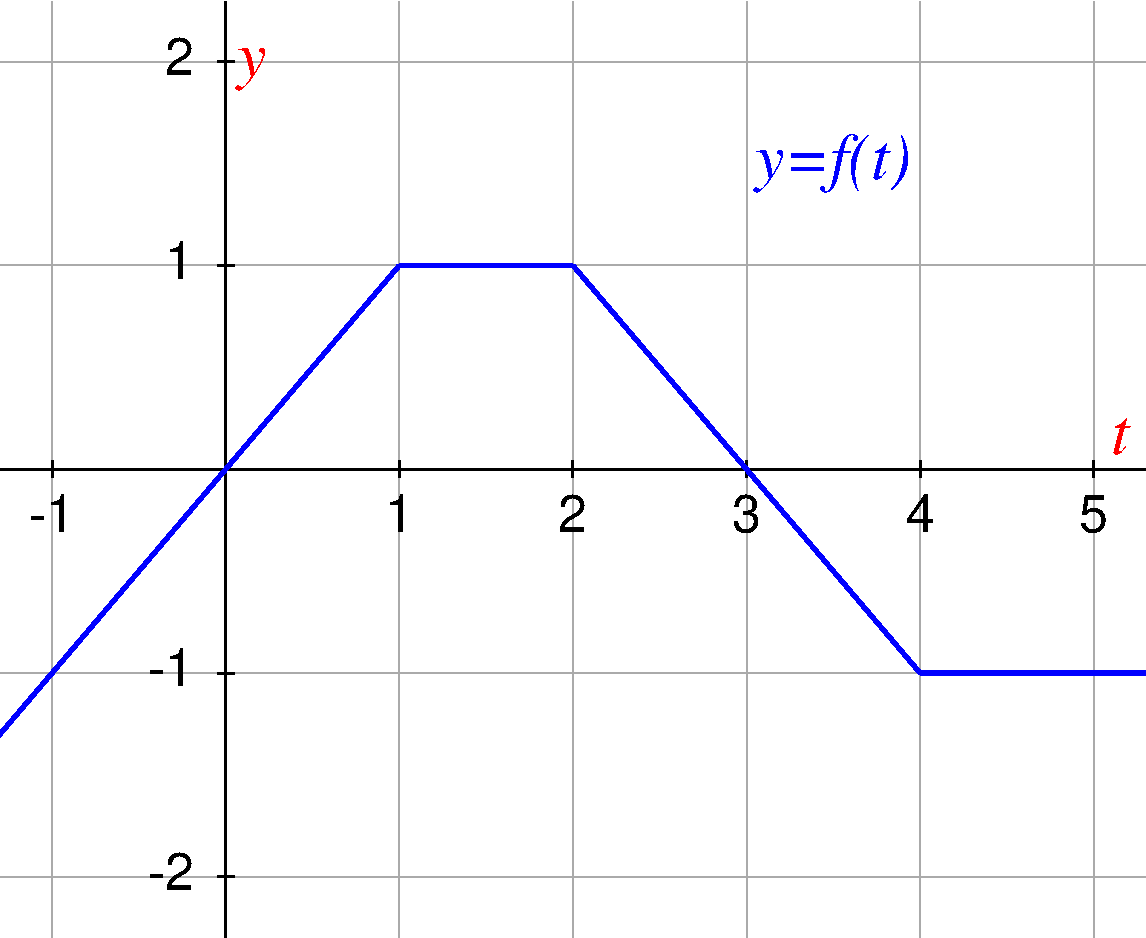
\includegraphics[scale=.4]{G21}
			\end{center}
		\end{column}

		\begin{column}{.3\textwidth}
			Compute:
			\begin{enumerate}
				\item $\displaystyle \int_{0}^{1}\! f(t) dt$

				\item $\displaystyle \int_{0}^{2}\! f(t) dt$

				\item $\displaystyle \int_{0}^{3}\! f(t) dt$

				\item $\displaystyle \int_{0}^{4}\! f(t) dt$

				\item $\displaystyle \int_{0}^{5}\! f(t) dt$
			\end{enumerate}
		\end{column}
	\end{columns}
\end{frame}

\begin{frame}[t]
	\fontsize{13}{13}\selectfont
	\frametitle{Towards FTC (continued)}

	\begin{center}
		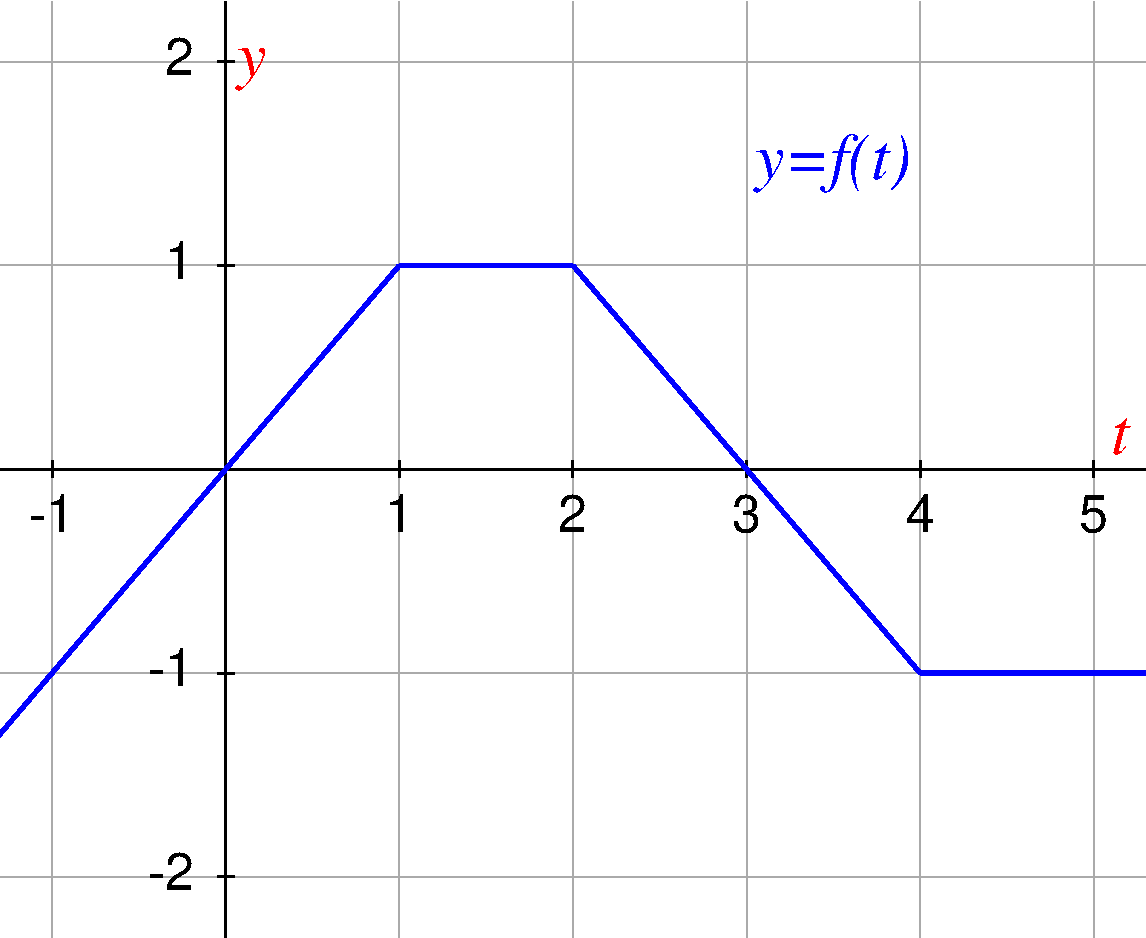
\includegraphics[width=8cm, height=5cm]{G21}
	\end{center}

	Call $\displaystyle F(x) = \int_{0}^{x}f(t) dt$. This is a new function.
	\begin{itemize}
		\item Sketch the graph of $\displaystyle y=F(x)$.

		\item Using the graph you just sketched, sketch the graph of
			$\displaystyle y=F'(x)$.
	\end{itemize}
\end{frame}

\begin{frame}[t]
	\frametitle{Filling the tank}

	A tank is being filled with water. At time $t$ water flows into the tank at a rate
	of
	\[
		A \, e^{-bt}\arctan (ct)
	\]
	litres per second, where $A$, $b$, and $c$ are constants. The amount of water in
	the tank at time $t=0s$ is $V_{0}$. Write an expression for the amount of
	water $V$ in the tank at time $t$.
\end{frame}

\begin{frame}[t]
	\fontsize{13}{13}\selectfont
	\frametitle{True or False?}

	\begin{enumerate}
		\item If $f$ is continuous on the interval $[a,b]$, then
			\[
				\frac{d}{dx}\left( \int_{a}^{b}f(t)dt\right)=f(x).
			\]

			\vspace{4mm}

		\item If $f$ is differentiable, then
			\[
				\frac{d}{dx}\left(\int_{a}^{x}f(t)\,dt \right) \; = \; \int_{a}^{x}f'(t)
				\,dt .
			\]
	\end{enumerate}
\end{frame}

\begin{frame}[t]
	\fontsize{13}{13}\selectfont
	\frametitle{More True or False}

	Let $f$ and $g$ be differentiable functions with domain $\displaystyle \mathbb{R}$.
	\\ Assume that $\displaystyle f'(x) = g(x)$ for all $x$. \\ Which of the following
	statements must be true?

	\begin{enumerate}
		\item $\displaystyle f(x) = \int_{0}^{x}g(t) dt$.

		\item If $\displaystyle f(0)=0$, then
			$\displaystyle f(x) = \int_{0}^{x}g(t) dt$.

		\item If $\displaystyle g(0)=0$, then
			$\displaystyle f(x) = \int_{0}^{x}g(t) dt$.

		\item There exists $C \in \mathbb{R}$ such that $\displaystyle f(x) = C + \int
			_{0}^{x}g(t) dt$.

		\item There exists $C\in \mathbb{R}$ such that $\displaystyle f(x) = C + \int
			_{1}^{x}g(t) dt$.
	\end{enumerate}
\end{frame}

\begin{frame}[t]
	\fontsize{11}{11}\selectfont
	\frametitle{True, False, or Shrug?}

	We want to find a function $H$ with domain $\mathbb{R}$ such that $\displaystyle
	H(1) = -2$ and such that $\displaystyle H'(x) = e^{\sin x}$ for all $x$.
	Decide whether each of the following statements is true, false, or we do not
	have enough information to decide.

	\begin{enumerate}
		\item The function $\displaystyle \quad H(x) = \int_{0}^{x}e^{\sin t}dt \quad$
			is a solution.

		\item The function $\displaystyle \quad H(x) = \int_{2}^{x}e^{\sin t}dt \quad$
			is a solution.

		\item $\forall C \in \mathbb{R}$, the function
			$\displaystyle \quad H(x) = \int_{0}^{x}e^{\sin t}dt + C \quad$ is a
			solution.

		\item $\exists C \in \mathbb{R}$ s.t.\ the function
			$\displaystyle \quad H(x) = \int_{0}^{x}e^{\sin t}dt + C \quad$ is a
			solution.

		\item The function $\displaystyle \quad H(x) = \int_{1}^{x}e^{\sin t}dt -2 \quad$
			is a solution.

		\item There is more than one solution.
	\end{enumerate}
\end{frame}

\begin{frame}[t]
	\fontsize{13}{13}\selectfont
	\frametitle{Examples of FTC-1}

	Compute the derivative of the following functions

	\begin{enumerate}
		\item $\displaystyle F_{1}(x) = \int_{0}^{1}e^{-t^2}dt$. \\
			\vfill

		\item $\displaystyle F_{2}(x) = \int_{0}^{x}e^{-\sin t}dt$. \\
			\vfill

		\item $\displaystyle F_{3}(x) = \int_{1}^{x^2}\frac{\sin t}{t^{2}}dt$. \\
			\vfill

		\item $\displaystyle F_{4}(x) = \! \int_{x}^{7}\sin^{3}\! \! \left( \sqrt{t}\right
			) \! dt$. \\
			\vfill

		\item $\displaystyle F_{5}(x) = \int_{2x}^{x^2}\frac{1}{1+t^{3}}dt$. \\
	\end{enumerate}
\end{frame}

\begin{frame}[t]
	\frametitle{A generalized version of FTC-1}

	Let $f$, $u$, $v$ be differentiable functions with domain $\mathbb{R}$. Let us
	call
	\[
		F(x) = \int_{u(x)}^{v(x)}f(t) dt
	\]
	Find a formula for
	\[
		F'(x)
	\]
	in terms of $f$, $u$, $v$, $f'$, $u'$, $v'$.
\end{frame}

\begin{frame}[t]
	\frametitle{An integral equation}

	Assume $f$ is a continuous function that satisfies, for every $x \in \mathbb{R}$:
	\[
		\int_{0}^{x}e^{t}f(t) = \frac{\sin x}{x^{2}+1}
	\]

	Find an explicit expression for $f(x)$.
\end{frame}

\begin{frame}[t]
	\frametitle{Compute these definite integrals}

	\begin{enumerate}
		\item $\displaystyle \int_{1}^{2}x^{3}dx$
			\vfill

		\item $\displaystyle \int_{0}^{1}\left[ e^{x}+ e^{-x}- \cos (2x) \right] dx$
			\vfill

		\item $\displaystyle \int_{1/2}^{1/\sqrt{2}}\frac{4}{\sqrt{1-x^{2}}}dx$
			\vfill

		\item $\displaystyle \int_{\pi/4}^{\pi/3}\sec^{2}x \; dx$
			\vfill

		\item $\displaystyle \int_{1}^{2}\left[ \frac{d}{dx}\left( \frac{\sin^{2}x }{1
			+ \arctan^{2}x + e^{-x^2}}\right) \right] dx$
			\vfill
	\end{enumerate}
\end{frame}

\begin{frame}[t]
	\frametitle{Find the error}

	\[
		\int_{-1}^{1}\frac{1}{x^{4}}dx \; = \; \left. \frac{-1}{3x^{3}}\right\vert_{-1}
		^{1}= \frac{-2}{3}
	\]

	However, $x^{4}$ is always positive, so the integral should be positive.
\end{frame}

\begin{frame}[t]
	\frametitle{Areas}

	Calculate the area of the bounded region...
	\vspace{.2cm}
	\begin{enumerate}
		\item ... between the $x$-axis and $\displaystyle y=4x-x^{2}$.
			\vspace{.2cm}

		\item ... between $y=\cos x$, the $x$-axis, from $x=0$ to $x=\pi$.
			\vspace{.2cm}

		\item ... between $\displaystyle y=x^{2}+3$ and $\displaystyle y=3x+1$.
			\vspace{.2cm}

		\item ... between $y=1$, the $y$-axis, and $y=\ln(x+1)$.
	\end{enumerate}
\end{frame}

\begin{frame}[t]
	\frametitle{Minimizing area}

	For each $a >0$ consider the function
	\[
		f_{a}(x) = 1 + a -ax^{2}
	\]

	Find the value of $a$ that minimizes the area of the region bounded by the graph
	of $f_{a}$ and the $x$-axis. \hfill
	\href{https://www.desmos.com/calculator/x7vkfcerdp}{\beamergotobutton{desmos}}
\end{frame}

\begin{frame}[t]
	\frametitle{Symmetry}

	Calculate the value of these integrals \emph{without computing any
	antiderivative}.

	\begin{enumerate}
		\begin{multicols}{3}
			\item $\displaystyle \int_{-2}^{2}\sin x^{3}dx$ \item $\displaystyle \int_{0}
			^{\pi}\cos^{2}x \, dx$ \item $\displaystyle \int_{-1}^{1}\arccos x \, dx$
		\end{multicols}
	\end{enumerate}

	\emph{Hint:} Sketch the graphs (use desmos) and use symmetry to compute the integral.
	\\ Once you guess the symmetry of the graph, try to write it algebraically.
	\hfill
	\href{https://www.desmos.com/calculator/ncysdsu3yv}{\beamergotobutton{1}}
	\href{https://www.desmos.com/calculator/fwjs5zoury}{\beamergotobutton{2}}
	\href{https://www.desmos.com/calculator/tjakgza6vf}{\beamergotobutton{3}}
\end{frame}

\begin{frame}[t]
	\fontsize{13}{13}\selectfont
	\frametitle{Average Velocity}

	You are traveling. \\ Your position at time $t$ is $s(t)$. \\ Your velocity at
	time $t$ is $v(t)$. \\ The function $v$ is continuous on an interval $[a,b]$.

	Which of the following represent your average velocity on $[a,b]$?

	\begin{enumerate}
		\item $\displaystyle \frac{s(b) - s(a)}{b-a}$

		\item $\displaystyle \frac{1}{b-a}\int_{a}^{b}v(t) dt$

		\item $v(c)$ for at least one $c$ between $a$ and $b$
	\end{enumerate}
\end{frame}

\begin{frame}[t]
	\fontsize{13}{13}\selectfont
	\frametitle{The Mean Value Theorem for integrals is back}

	Prove the following theorem.

	\begin{block}{\fontsize{13}{13}\selectfont Theorem}
		Let $a < b$. Let $f$ be a continuous function on $[a,b]$. \\ There exists $c
		\in [a,b]$ such that
		\vspace{-.5cm}
		\[
			f(c) \; = \; \frac{1}{b-a}\int_{a}^{b}f(t) dt
		\]
	\end{block}

	% \pause

	\emph{Hint:} Use MVT for the function
	$\displaystyle F(x) = \int_{a}^{x}f(t) dt$.
\end{frame}

\begin{frame}[t]
	\frametitle{Warm up}

	Calculate
	\[
		\int \frac{\sin \sqrt{x}}{\sqrt{x}}\, dx
	\]

	\emph{Hint:} Use the substitution $\displaystyle u=\sqrt{x}$.
\end{frame}

\begin{frame}[t]
	\frametitle{Computation practice: integration by substitution}

	Use substitutions to compute:
	\begin{multicols}{2}
		\begin{enumerate}
			\item $\displaystyle \int \frac{\sin \sqrt{x}}{\sqrt{x}}dx$
				\vspace{.2cm}

			\item $\displaystyle \int e^{x}\cos \left(e^{x}\right) dx$
				\vspace{.2cm}

			\item $\displaystyle \int \cot x \, dx$
				\vspace{.2cm}

			\item $\displaystyle \int x^{2}\sqrt{x+1}\, dx$
				\vspace{.2cm}
			% \pause

			\item $\displaystyle \int \frac{e^{2x}}{\sqrt{e^{x}+ 1}}\, dx$
				\vspace{.2cm}

			\item $\displaystyle \int \frac{\left( \ln \ln x \right)^{2}}{ x \ln x}\, d
				x$
				\vspace{.2cm}

			\item $\displaystyle \int x e^{-x^2}\, dx$
				\vspace{.2cm}

			\item $\displaystyle \int e^{-x^2}\, dx$
				\vspace{.2cm}
		\end{enumerate}
	\end{multicols}
\end{frame}

\begin{frame}
	\fontsize{13}{13}\selectfont
	\frametitle{Definite integral via substitution}

	This final answer is right, but the write-up is WRONG. Why?
	\vfill

	Calculate $\displaystyle I = \int_{0}^{2}\sqrt{x^{3}+1}\; x^{2}dx$
	\begin{block}{Wrong answer}
		Substitution: $\displaystyle u = x^{3}+1, \; du=3x^{2}dx$.
		\begin{align*}
			I \; & = \; \frac{1}{3}\int_{0}^{2}\sqrt{x^{3}+1}\; (3x^{2}dx)                             &  & = \; \frac{1}{3}\int_{0}^{2}u^{1/2}\; du                             \\
			     & = \; \frac{1}{3}\; \frac{2}{3}\; \left. u^{3/2}\right\vert_{0}^{2}                  &  & = \; \left. \frac{1}{9}\left(x^{3}+1\right)^{2/3}\right\vert_{0}^{2} \\
			     & = \; \frac{2}{9}\left( 2^{3}+ 1 \right)^{3/2}- \frac{2}{9}\left( 0 + 1\right)^{3/2} &  & = \; \frac{52}{9}
		\end{align*}
	\end{block}
\end{frame}

\begin{frame}[t]
	\fontsize{13}{13}\selectfont
	\frametitle{Integral of products of $\sin$ and $\cos$}
	We want to compute
	\vspace{-.5cm}
	\[
		I = \int \sin^{3}x \cos^{2}x \, dx
	\]

	\begin{enumerate}
		\item Attempt the substitution $\displaystyle u = \sin x$

		\item Attempt the substitution $\displaystyle u = \cos x$

		\item One worked better than the other. Which one? Why? \\ Finish the
			problem.
		% \pause

		\item Assume we want to compute
			\[
				\int \sin^{n}x \cos^{m}x \, dx
			\]
			When will the substitution $\displaystyle u = \sin x$ be helpful? \\ When
			will the substitution $\displaystyle u = \cos x$ be helpful?
	\end{enumerate}
\end{frame}

\begin{frame}[t]
	\fontsize{13}{13}\selectfont
	\frametitle{Odd functions}

	\begin{block}{Theorem}
		Let $f$ be a continuous function. Let $a >0$. IF $f$ is odd, THEN
		\[
			\int_{-a}^{a}f(x) dx = 0
		\]
	\end{block}

	% \pause

	\begin{enumerate}
		\item Write down the definition of ``odd function".

		\item Draw a picture to interpret the theorem geometrically.

		\item Prove the theorem!

			\emph{Hint:} Write the integral as sum of two pieces. Use a substitution to
			show that one of the two pieces equals minus the other.
	\end{enumerate}
\end{frame}

\begin{frame}[t]
	\frametitle{Computation practice: Integration by parts}

	Use integration by parts (possibly in combination with other methods) to
	compute:
	\begin{multicols}{2}
		\begin{enumerate}
			\item $\displaystyle \int x e^{-2x}dx$
				\vspace{.2cm}

			\item $\displaystyle \int x^{2}\sin x \, dx$
				\vspace{.2cm}

			\item $\displaystyle \int \ln x \, dx$
				\vspace{.2cm}

			\item $\displaystyle \int \sin \sqrt{x}\, dx$
				\vspace{.2cm}
			% \pause

			\item $\displaystyle \int x \arctan x \, dx$
				\vspace{.2cm}

			\item $\displaystyle \int x^{2}\arcsin x \, dx$
				\vspace{.2cm}

			\item $\displaystyle \int e^{\cos x}\sin^{3}x \, dx$
				\vspace{.2cm}

			\item $\displaystyle \int e^{ax}\sin (bx) dx$
				\vspace{.2cm}
		\end{enumerate}
	\end{multicols}
\end{frame}

\begin{frame}[t]
	\frametitle{Persistence}
	Compute
	\begin{multicols}{2}
		\begin{itemize}
			\item $\displaystyle \int_{1}^{e}\left( \ln x \right)^{3}dx$
				% \pause
				\vspace{.2cm}

			\item $\displaystyle \int_{1}^{e}\left( \ln x \right)^{10}dx$
		\end{itemize}
	\end{multicols}
	% \pause
	There is a more efficient approach. Call
	\[
		I_{n}= \int_{1}^{e}\left( \ln x \right)^{n}dx
	\]
	Use integration by parts on $I_{n}$. You will get an equation with $I_{n}$ and
	$I_{n-1}$. Now solve the previous questions.

	\vfill
	\hfill \href{https://oeis.org/}{\beamergotobutton{OEIS}}
\end{frame}

\begin{frame}[t]
	\frametitle{Integrals from a graph}

	\begin{columns}
		\begin{column}{.7\textwidth}
			\begin{center}
				\only<1>{
				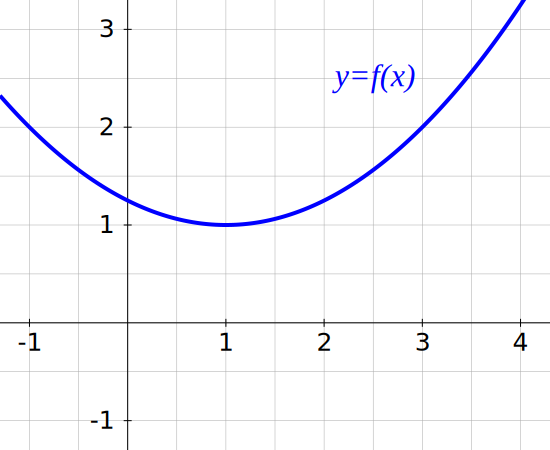
\includegraphics[scale=.4]{G22}
				} \only<2>{
				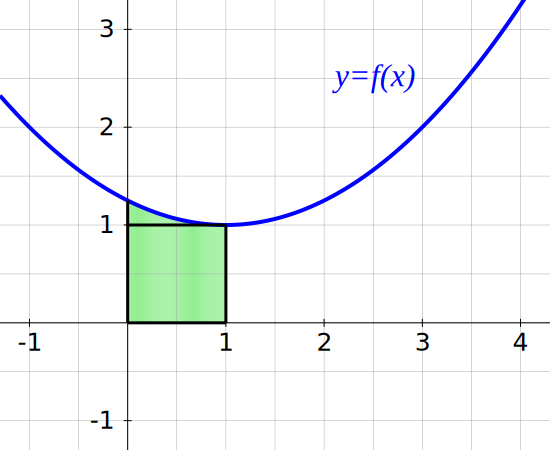
\includegraphics[scale=.4]{G22a}
				} \only<3>{
				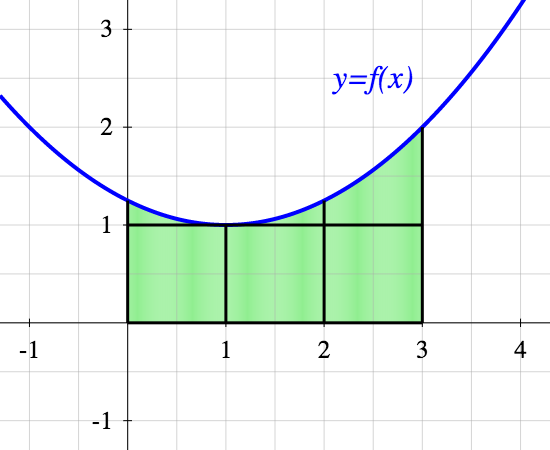
\includegraphics[scale=.4]{G22b}
				}
			\end{center}
		\end{column}

		\begin{column}{.32\textwidth}
			Estimate:
			\begin{enumerate}
				\item $\displaystyle \int_{0}^{1}f(x) dx$

				\item $\displaystyle \int_{0}^{1}f'(x) dx$

				\item $\displaystyle \int_{0}^{3}x \, f'(x) dx$

				\item $\displaystyle \int_{0}^{1}f(3x) dx$
			\end{enumerate}
		\end{column}
	\end{columns}
\end{frame}

\begin{frame}[t]
	\frametitle{The error function}

	The following function is tabulated.
	\[
		{\Large E(x) = \int_0^x e^{-t^2} dt}.
	\]
	Write the following quantities in terms of $E$:

	\begin{multicols}{2}
		\begin{enumerate}
			\item $\displaystyle \int_{1}^{2}e^{-t^2}dt$

				\vspace{.2cm}

			\item $\displaystyle \int_{0}^{x}t^{2}e^{-t^2}dt$

				\vspace{.2cm}

			\item $\displaystyle \int_{0}^{x}e^{-2t^2}dt$

				\vspace{.2cm}
			% \pause

			\item $\displaystyle \int_{0}^{1}e^{-t^2+6t}dt$

				\vspace{.2cm}

			\item $\displaystyle \int_{x_1}^{x_2}e^{-\frac{(t- \mu)^{2}}{\sigma^{2}}}dt$

				\vspace{.2cm}

			\item $\displaystyle \int_{1}^{2}\frac{e^{-t}}{\sqrt{t}}dt$
		\end{enumerate}
	\end{multicols}
\end{frame}

\begin{frame}[t]
	\frametitle{Exp-trig antiderivative}

	We want to compute
	\[
		I = \int e^{ax}\sin (bx) \; dx
	\]
	\begin{itemize}
		\item Try once integration by parts choosing $\displaystyle u = e^{ax}$.
			Stop.

		\item Go back to $I$. Now try integration by parts once choosing
			$\displaystyle u = \sin (bx)$ instead. Stop.

		\item Look at what you did. Think.
	\end{itemize}
\end{frame}

\begin{frame}[t]
	\fontsize{13}{13}\selectfont
	\frametitle{Practice: Integrals with trigonometric functions}

	Compute the following antiderivatives. (Once you get them to a form from where
	you see a path to finish them, even if long, you may stop.)

	\begin{multicols}{2}
		\begin{enumerate}
			\item $\displaystyle \int \sin^{10}x \cos x \ dx$
				\vspace{.2cm}

			\item $\displaystyle \int \sin^{10}x \cos^{7}x \, dx$
				\vspace{.2cm}

			\item $\displaystyle \int e^{\cos x}\cos x \sin^{3}x \, dx$
				\vspace{.2cm}

			\item $\displaystyle \int \cos^{2}x \, dx$
				\vspace{.2cm}

			\item $\displaystyle \int \cos^{4}x \, dx$
				\vspace{.2cm}

			\item $\displaystyle \int \csc x \, dx$
				\vspace{.2cm}
		\end{enumerate}
	\end{multicols}

	\vspace{-.5cm}
	{\fontsize{10}{10}\selectfont \begin{block}{ \fontsize{12}{12}\selectfont Useful trig identities}\vspace{-.5cm} \begin{align*}\large&\sin^{2}x + \cos^{2}x = 1&\sin^{2}x&= \frac{1 - \cos (2x)}{2}\\&\tan^{2}x + 1 = \sec^{2}x&\cos^{2}x&= \frac{1 + \cos (2x)}{2}\end{align*}\end{block} }
\end{frame}

\begin{frame}[t]
	\frametitle{Integral of products of secant and tangent}

	To integrate
	\[
		\int \sec^{n}x \tan^{m}x \, dx
	\]
	\begin{itemize}
		\item If \boxed{\phantom{spacespace}}, then use the substitution $\displaystyle
			u = \tan x$.

		\item If \boxed{\phantom{spacespace}}, then use the substitution $\displaystyle
			u = \sec x$.
	\end{itemize}

	\vfill

	{\fontsize{13}{13}\selectfont \emph{Hint:} You will need \begin{itemize}\begin{multicols}{2}\item $\displaystyle \frac{d}{dx}\left[ \tan x \right] = \ldots$ \item $\displaystyle \frac{d}{dx}\left[ \sec x \right] = \ldots$\end{multicols}

	\item The trig identity involving $\sec$ and $\tan$\end{itemize} }
\end{frame}

\begin{frame}[t]
	\fontsize{13}{13}\selectfont
	\frametitle{A reduction formula}

	Let $\displaystyle I_{n}= \int_{0}^{2\pi}\sin^{n}x \, dx$.
	\vspace{.3cm}

	\begin{enumerate}
		\item Compute $I_{0}$ and $I_{1}$.
			\vspace{.3cm}

		\item Write an equation for $\displaystyle I_{n}$ in terms of $\displaystyle
			I_{n-2}$. This is called a reduction formula.
			\vspace{.3cm}

			\emph{Hint:} Starting with $I_{n}$, use integration by parts once. \\ Then
			use $\displaystyle \sin^{2}x + \cos^{2}x = 1$ to rewrite the new integral in
			terms of $\displaystyle I_{n}$ and $\displaystyle I_{n-2}$.
			\vspace{.3cm}

		\item Write a a formula for $I_{n}$ for all natural numbers $n$.

		%\DS{I_8 = \frac{35}{64} \pi}.
	\end{enumerate}
\end{frame}

\begin{frame}[t]
	\frametitle{A different kind of substitution}

	Calculate
	\[
		\int_{0}^{1}\sqrt{1 - x^{2}}\; dx
	\]
	using the substitution
	\[
		\begin{cases}
			x = \sin \theta \\
			dx = ??
		\end{cases}
	\]
\end{frame}

\begin{frame}[t]
	\fontsize{13}{13}\selectfont
	\frametitle{Rational integrals}

	\begin{enumerate}
		\item Calculate $\displaystyle \int \frac{1}{x+a}\, dx$
			\vspace{.2cm}

		\item Reduce to common denominator \, $\displaystyle \frac{2}{x}- \frac{3}{x+3}$
			\vspace{.2cm}

		\item Calculate $\displaystyle \int \frac{-x + 6}{x^{2}+ 3x}\, dx$
			\vspace{.2cm}

		\item Calculate $\displaystyle \int \frac{1}{x^{2}+ 3x}\, dx$
			\vspace{.2cm}

		\item Calculate $\displaystyle \int \frac{1}{x^{3}-x}\, dx$
	\end{enumerate}
\end{frame}

\begin{frame}[t]
	\fontsize{13}{13}\selectfont
	\frametitle{Repeated factors}

	\begin{enumerate}
		\item Calculate $\displaystyle \int \frac{1}{(x+1)^{n}}\, dx$ \quad for $n >1$
			\vspace{.2cm}

		\item Calculate $\displaystyle \int \frac{(x+1) - 1}{(x+1)^{2}}\, dx$
			\vspace{.2cm}

		\item Calculate $\displaystyle \int \frac{2x + 6}{(x+1)^{2}}\, dx$
			\vspace{.2cm}

		\item Calculate $\displaystyle \int \frac{x^{2}}{(x+1)^{3}}\, dx$
	\end{enumerate}
\end{frame}

\begin{frame}[t]
	\fontsize{13}{13}\selectfont
	\frametitle{Irreducible quadratics}

	\begin{enumerate}
		\item Calculate $\displaystyle \int \frac{1}{x^{2}+ 1}\, dx$ and $\displaystyle
			\int \frac{x}{x^{2}+1}\, dx$.
			\vspace{.2cm}

			\emph{Hint:} These two are very short.
			\vspace{.2cm}

		\item Calculate $\displaystyle \int \frac{2x+ 3}{x^{2}+ 1}\, dx$
			\vspace{.2cm}

		\item Calculate $\displaystyle \int \frac{x^{2}}{x^{2}+ 1}\, dx$
			\vspace{.2cm}

		\item Calculate $\displaystyle \int \frac{x}{x^{2}+ x + 1 }\, dx$
			\vspace{.2cm}

			\emph{Hint:} Complete the square in the denominator and use a substitution
			to transform into one of the previous ones.
	\end{enumerate}
\end{frame}

\begin{frame}[t]
	\frametitle{Repeated quadratics}

	\begin{enumerate}
		\item Calculate
			\[
				\frac{d}{dx}\left[ \arctan x \right], \quad \quad \frac{d}{dx}\left[ \frac{x}{1+x^{2}}
				\right].
			\]

		\item Use the previous answer to calculate
			\[
				\int \frac{1}{\left(1+x^{2}\right)^{2}}\; dx
			\]
	\end{enumerate}
\end{frame}

\begin{frame}[t]
	\frametitle{The integral of secant}

	Compute
	\[
		\int \sec x \, dx
	\]
	using the substitution $\displaystyle u = \sin x$.
\end{frame}

\begin{frame}[t]
	\frametitle{Messier rational functions}

	\begin{enumerate}
		\item How could we compute an integral of the form
			\[
				\int \frac{\text{polynomial}}{(x+1)^{3}(x+2)}\, dx \; ?
			\]

		\item How could we compute an integral of the form
			\[
				\int \frac{\text{polynomial}}{x^{4}(x+1)^{3}(x+2)(x^{2}+1)(x^{2}+4)}\,dx
				\; ?
			\]
	\end{enumerate}
\end{frame}

\begin{frame}[t]
	\frametitle{An equation for volumes by the carrot method}

	Let $a < b$.

	Let $f$ be a continuous, positive function defined on $[a,b]$.

	Let $R$ be the region in the first quadrant bounded between the graph of $f$ and
	the $x$-axis.

	Find a formula for the volume of the solid of revolution obtained by rotation the
	region $R$ around the $x$-axis.
\end{frame}

\begin{frame}[t]
	\frametitle{Sphere}

	You know the formula for the volume of a sphere with radius $R$. Now you are able
	to prove it!

	\begin{enumerate}
		\item Write an equation for the circle with radius $R$ centered at $(0,0)$.

		\item If you rotate this circle around the $x$-axis, it will produce a
			sphere. Compute its volume as an integral by slicing it like a carrot.
	\end{enumerate}
\end{frame}

\begin{frame}[t]
	\frametitle{Pyramid}

	Compute the volume of a pyramid with height $H$ and square base with side
	length $L$.

	\emph{Hint:} Slice the pyramid like a carrot with cuts parallel to the base.
\end{frame}

\begin{frame}[t]
	\frametitle{Many axis of rotation}

	Let $R$ be the region in the first quadrant bounded between the curves with
	equations $\displaystyle y = x^{3}$ and $\displaystyle y=\sqrt{32x}$.

	Compute the volume of the solid of revolution obtained by rotating $R$ around...
	\begin{enumerate}
		\item ... the $x$-axis

		\item ... the $y$-axis

		\item ... the line $y=-1$
	\end{enumerate}
\end{frame}

\begin{frame}[t]
	\frametitle{An equation for volumes by ``cylindrical shells"}

	Let $a < b$.

	Let $f$ be a continuous, positive function defined on $[a,b]$.

	Let $R$ be the region in the first quadrant bounded between the graph of $f$ and
	the $x$-axis.

	Find a formula for the volume of the solid of revolution obtained by rotation the
	region $R$ around the $y$-axis.
\end{frame}

\begin{frame}[t]
	\frametitle{A hat}

	Let $R$ be the region in the first quadrant bounded between the graphs of
	$\displaystyle y=x^{5}+x-2$, $\displaystyle x=2$, and the $\displaystyle x$-axis.

	Compute the volume of the solid of revolution obtained by rotating $R$ around
	the $y$-axis.
\end{frame}

\begin{frame}[t]
	\fontsize{13}{13}\selectfont
	\frametitle{Doughnut}

	Let $R$ be the region inside the curve with equation
	\[
		(x-1)^{2}+ y^{2}=1.
	\]
	Rotate $R$ around the line with equation $\displaystyle x=4$. The resulting
	solid is called a \emph{torus}.

	\begin{enumerate}
		\item Draw a picture and convince yourself that a torus looks like a doughnut.

		\item Set up the volume of the torus as an integral using $x$ as the variable
			(``cylindrical shell method"). You do not need to compute the integral.

		\item Set up the volume of the torus as an integral using $y$ as the variable
			(``carrot method"). You do not need to compute the integral.
	\end{enumerate}
\end{frame}

\begin{frame}[t]
	\frametitle{Challenge}

	Two cylinders have the same radius $R$ and their axes are perpendicular. Find the
	volume of their intersection.

	\emph{Hint:} You can slice the resulting solid by parallel cuts in three
	different directions. One of the three makes the problem much, much simpler
	than the other two.
\end{frame}

\begin{frame}[t]
	\frametitle{Warm up}

	Write a formula for the general term of these sequences
	\vfill
	\begin{enumerate}
		\item $\displaystyle \{a_{n}\}_{n=0}^{\infty}= \{ \, 1, \, 4, \, 9, \, 16, \,
			25, \, \ldots \, \}$
			\vfill

		\item $\displaystyle \{b_{n}\}_{n=1}^{\infty}= \{ \, 1, \, -2, \, 4, \, -8, \,
			16, \, -32, \, \ldots \, \}$
			\vfill

		\item $\displaystyle \{c_{n}\}_{n=1}^{\infty}= \left\{ \, \frac{2}{1!}, \, \frac{3}{2!}
			, \, \frac{4}{3!}, \, \frac{5}{4!}, \, \ldots \, \right\}$
			\vfill

		\item $\displaystyle \{d_{n}\}_{n=1}^{\infty}= \{ \, 1, \, 4, \, 7, \, 10, \,
			13, \, \ldots \, \}$
	\end{enumerate}
\end{frame}

\begin{frame}[t]
	\frametitle{Sequences vs functions -- convergence}

	For any function $f$ with domain $[0, \infty)$, \\ we define a sequence as $a_{n}
	= f(n)$. \\ Let $L \in \mathbb{R}$. Which of these implications is true?

	\begin{enumerate}
		\item IF $\displaystyle \lim_{x \to \infty}f(x) = L$, \; THEN
			$\displaystyle \lim_{n \to \infty}a_{n}= L$.
			\vfill

		\item IF $\displaystyle \lim_{n \to \infty}a_{n}= L$, \; THEN
			$\displaystyle \lim_{x \to \infty}f(x) = L$.
			\vfill

		\item IF $\displaystyle \lim_{n \to \infty}a_{n}= L$, \; THEN
			$\displaystyle \lim_{n \to \infty}a_{n+1}= L$.
	\end{enumerate}
\end{frame}

\begin{frame}[t]
	\fontsize{13}{13}\selectfont
	\frametitle{Definition of limit of a sequence}

	Let $\displaystyle \left\{ a_{n} \right\}_{n=0}^{\infty}$ be a sequence. Let
	$\displaystyle L \in \mathbb{R}$. \\ Which statements are equivalent to $\displaystyle
	``\left\{ a_{n} \right\}_{n=0}^{\infty}\longrightarrow L"$?

	\begin{enumerate}
		\item $\displaystyle \forall \varepsilon>0, \; \exists n_{0}\in \mathbb{N}, \;
			\forall n \in \mathbb{N}, \; \quad n \geq n_{0}\implies |L-a_{n}| < \varepsilon
			.$

		\item $\displaystyle \forall \varepsilon>0, \; \exists n_{0}\in \mathbb{N}, \;
			\forall n \in \mathbb{N}, \; \quad n \;{\color{red} > }\; n_{0}\implies |L-
			a_{n}| < \varepsilon.$

		\item $\displaystyle \forall \varepsilon>0, \; \exists n_{0}\in{\color{red} \mathbb{R}}
			, \; \forall n \in \mathbb{N}, \; \quad n \geq n_{0}\implies |L-a_{n}| < \varepsilon
			.$

		\item $\displaystyle \forall \varepsilon>0, \; \exists n_{0}\in \mathbb{N}, \;
			\forall n \in{\color{red} \mathbb{R}}, \; \quad n \geq n_{0}\implies |L-a_{n}
			| < \varepsilon.$

		\item $\displaystyle \forall \varepsilon>0, \; \exists n_{0}\in \mathbb{N}, \;
			\forall n \in \mathbb{N}, \; \quad n \geq n_{0}\implies |L-a_{n}| \;{\color{red} \leq}
			\; \varepsilon.$

		\item $\displaystyle \forall \varepsilon \;{\color{red} \in (0,1)}, \; \exists
			n_{0}\in \mathbb{N}, \; \forall n \in \mathbb{N}, \; \quad n \geq n_{0}\implies
			|L-a_{n}| < \varepsilon.$

		\item $\displaystyle \forall \varepsilon>0, \; \exists n_{0}\in \mathbb{N}, \;
			\forall n \in \mathbb{N}, \; \quad n \geq n_{0}\implies |L-a_{n}| <{\color{red} \frac{1}{\varepsilon}}
			.$

		\item $\displaystyle \forall{\color{red} k \in \mathbb{Z}^{+}}, \; \exists n_{0}
			\in \mathbb{N}, \; \forall n \in \mathbb{N}, \; \quad n \geq n_{0}\implies
			|L-a_{n}| <{\color{red} k}.$

		\item $\displaystyle \forall{\color{red} k \in \mathbb{Z}^{+}}, \; \exists n_{0}
			\in \mathbb{N}, \; \forall n \in \mathbb{N}, \; \quad n \geq n_{0}\implies
			|L-a_{n}| <{\color{red} \frac{1}{k}}.$
	\end{enumerate}
\end{frame}

\begin{frame}[t]
	\fontsize{12}{12}\selectfont
	\frametitle{Definition of limit of a sequence (continued)}

	Let $\displaystyle \left\{ a_{n} \right\}_{n=0}^{\infty}$ be a sequence. Let
	$\displaystyle L \in \mathbb{R}$. \\ Which statements are equivalent to $\displaystyle
	``\left\{ a_{n} \right\}_{n=0}^{\infty}\longrightarrow L"$?

	\begin{enumerate}
		\addtocounter{enumi}{9}

		\item $\displaystyle \forall \varepsilon >0$, the interval
			$\displaystyle (L-\varepsilon, L+\varepsilon)$ contains all the elements
			of the sequence, except the first few.

		\item $\displaystyle \forall \varepsilon >0$, the interval
			$\displaystyle (L-\varepsilon, L+\varepsilon)$ contains infinitely many of
			the elements of the sequence.

		\item $\displaystyle \forall \varepsilon >0$, the interval
			$\displaystyle (L-\varepsilon, L+\varepsilon)$ contains \emph{{\color{red} almost all}}
			the elements of the sequence.

		\item $\displaystyle \forall \varepsilon >0$, the interval
			$\displaystyle [L-\varepsilon, L+\varepsilon]$ contains \emph{{\color{red} almost all}}
			the elements of the sequence.

		\item Every interval that contains $L$ must contain \emph{{\color{red} almost all}}
			all the elements of the sequence.

		\item Every open interval that contains $L$ must contain \emph{{\color{red} almost all}}
			all the elements of the sequence.
	\end{enumerate}

	\emph{Notation:} ``\emph{{\color{red} almost all}}" = ``all, except finitely
	many"
\end{frame}

\begin{frame}[t]
	\frametitle{Convergence and divergence}

	Let $\displaystyle \left\{ a_{n} \right\}_{n=0}^{\infty}$ be a sequence. \\ Write
	the formal definition of the following concepts:

	\begin{enumerate}
		\item $\displaystyle \left\{ a_{n} \right\}_{n=0}^{\infty}$ is convergent.

			\vfill

		\item $\displaystyle \left\{ a_{n} \right\}_{n=0}^{\infty}$ is divergent.

			\vfill

		\item $\displaystyle \left\{ a_{n} \right\}_{n=0}^{\infty}$ is divergent to $\infty$.

			\vfill
	\end{enumerate}
\end{frame}

\begin{frame}[t]
	\frametitle{Proof from the definition of limit}

	Prove, directly from the definition of limit, that
	\[
		\lim_{n \to \infty}\frac{n^{2}}{n^{2}+1}= 1.
	\]

	\emph{Suggestion:}
	\begin{enumerate}
		\item Write down the definition of what you want to show.

		\item Use itto decide the structure of the proof.

		\item Do some rough work if necessary.

		\item Write down the formal proof.
	\end{enumerate}
\end{frame}

\begin{frame}[t]
	\frametitle{Sequences vs functions -- monotonicity and boundness}

	For any function $f$ with domain $[0, \infty)$, \\ we define a sequence as $a_{n}
	= f(n)$. \\ Which of these implications is true?

	\begin{enumerate}
		\item IF $f$ is increasing, THEN
			$\displaystyle \left\{ a_{n} \right\}_{n=0}^{\infty}$ is increasing.
			\vfill

		\item IF $\displaystyle \left\{ a_{n} \right\}_{n=0}^{\infty}$ is increasing,
			THEN $f$ is increasing.
			\vfill

		\item IF $f$ is bounded, THEN
			$\displaystyle \left\{ a_{n} \right\}_{n=0}^{\infty}$ is bounded.
			\vfill

		\item IF $\displaystyle \left\{ a_{n} \right\}_{n=0}^{\infty}$ is bounded,
			THEN $f$ is bounded.
			\vfill
	\end{enumerate}
\end{frame}

\begin{frame}[t]
	\fontsize{13}{13}\selectfont
	\frametitle{Examples}

	Construct 8 examples of sequences. \\ If any of them is impossible, cite a theorem
	to justify it.

	\begin{center}
		\begin{tabular}{|c|c|c|c|}
			\hline
			                               &           & convergent                                               & divergent                                                \\
			\hline
			\multirow{2}{*}{monotonic}     & bounded   & \phantom{$\displaystyle \int_{\dfrac 11}^{9}$ ???????? } & \phantom{$\displaystyle \int_{\dfrac 11}^{9}$ ???????? } \\
			\cline{2-4}                    & unbounded & \phantom{$\displaystyle \int_{\dfrac 11}^{9}$ ???????? } & \phantom{$\displaystyle \int_{\dfrac 11}^{9}$ ???????? } \\
			\hline
			\multirow{2}{*}{not monotonic} & bounded   & \phantom{$\displaystyle \int_{\dfrac 11}^{9}$ ???????? } & \phantom{$\displaystyle \int_{\dfrac 11}^{9}$ ???????? } \\
			\cline{2-4}                    & unbounded & \phantom{$\displaystyle \int_{\dfrac 11}^{9}$ ???????? } & \phantom{$\displaystyle \int_{\dfrac 11}^{9}$ ???????? } \\
			\hline
		\end{tabular}
	\end{center}
\end{frame}

\begin{frame}[t]
	\frametitle{A sequence defined by recurrence}

	Consider the sequence $\displaystyle \left\{ R_{n} \right\}_{n=0}^{\infty}$
	defined by
	\begin{equation*}
		\begin{cases}
			                                & R_{0}= 1                           \\
			\forall n \in \mathbb{N}, \quad & R_{n+1}= \dfrac{ R_n + 2}{R_n + 3}
		\end{cases}
	\end{equation*}
	Compute $\displaystyle R_{1}, \, R_{2}, \, R_{3}$.
\end{frame}

\begin{frame}[t]
	\fontsize{13}{13}\selectfont
	\frametitle{Is this proof correct?}
	Let $\displaystyle \left\{ R_{n} \right\}_{n=0}^{\infty}$ be the sequence in
	the previous slide.
	\begin{block}{Claim:}
		$\displaystyle \left\{ R_{n} \right\}_{n=0}^{\infty}\longrightarrow -1 + \sqrt{3}$.
	\end{block}
	% \pause
	\begin{proof}
		\begin{multicols}{2}
			\begin{itemize}
				\item Let $\displaystyle L = \lim_{n \to \infty}R_{n}$.

				\item $\displaystyle R_{n+1}= \frac{R_{n}+ 2}{ R_{n}+ 3}$

				\item $\displaystyle \lim_{n \to \infty }R_{n+1}= \lim_{n \to \infty }\frac{R_{n}+
					2}{ R_{n}+ 3}$

				\item $\displaystyle L = \frac{L + 2}{ L + 3}$

				\item $\displaystyle L(L+3) = L + 2$

				\item $\displaystyle L^{2}+2L - 2 = 0$

				\item $\displaystyle L = -1 \pm \sqrt{3}$

				\item $\displaystyle L$ must be positive, so
					$\displaystyle L = -1 + \sqrt{3}$
			\end{itemize}
		\end{multicols}
	\end{proof}
\end{frame}

\begin{frame}[t]
	\frametitle{Another sequence defined by recurrence}
	Consider the sequence $\displaystyle \left\{ a_{n} \right\}_{n=0}^{\infty}$ defined
	by
	\begin{equation*}
		\begin{cases}
			                                & a_{0}= 1           \\
			\forall n \in \mathbb{N}, \quad & a_{n+1}= 1 - a_{n}
		\end{cases}
	\end{equation*}

	\begin{itemize}
		\item Use the same method as in the previous slide to compute its limit.

		\item {\bfseries After} you have computed the limit, calculate $a_{1}$, $a_{2}$,
			$a_{3}$, and $a_{4}$.

		\item What happened?
	\end{itemize}
\end{frame}

\begin{frame}[t]
	\frametitle{The original sequence defined by recurrence -- done right}

	Consider the sequence $\displaystyle \left\{ R_{n} \right\}_{n=0}^{\infty}$
	defined by
	\begin{equation*}
		\begin{cases}
			                                & R_{0}= 1                           \\
			\forall n \in \mathbb{N}, \quad & R_{n+1}= \dfrac{ R_n + 2}{R_n + 3}
		\end{cases}
	\end{equation*}

	\begin{enumerate}
		\item Prove $\displaystyle \left\{ R_{n} \right\}_{n=0}^{\infty}$ is bounded
			below by 0.

		\item Prove $\displaystyle \left\{ R_{n} \right\}_{n=0}^{\infty}$ is decreasing
			(use induction)

		\item Prove $\displaystyle \left\{ R_{n} \right\}_{n=0}^{\infty}$ is convergent
			(use a theorem)

		\item Now the calculation in the earlier slide is correct, and we can get
			the value of the limit.
	\end{enumerate}
\end{frame}

\begin{frame}[t]
	\fontsize{13}{13}\selectfont
	\frametitle{\fontsize{13}{13}\selectfont True or False - convergence,
	monotonicity, and boundedness}

	\begin{enumerate}
		\item If a sequence is convergent, then it is bounded above.

		\item If a sequence is bounded, then it is convergent

		\item If a sequence is convergent, then it is eventually monotonic.

		\item If a sequence is positive and converges to 0, then it is eventually
			monotonic.

		\item If a sequence diverges to $\infty$, then it is eventually monotonic.

		\item If a sequence diverges, then it is unbounded.

		\item If a sequence diverges and is unbounded above, then it diverges to
			$\infty$.

		\item If a sequence is eventually monotonic, then it is either convergent, divergent
			to $\infty$, or divergent to $-\infty$.
	\end{enumerate}
\end{frame}

\begin{frame}[t]
	\frametitle{True or False - Rapid fire}

	\begin{enumerate}
		\item (convergent) $\displaystyle \implies$ (bounded)
			\vfill

		\item (convergent) $\displaystyle \implies$ (monotonic)
			\vfill

		\item (convergent) $\displaystyle \implies$ (eventually monotonic)
			\vfill

		\item (bounded) $\displaystyle \implies$ (convergent)
			\vfill

		\item (monotonic) $\displaystyle \implies$ (convergent)
			\vfill

		\item (bounded + monotonic) $\displaystyle \implies$ (convergent)
			\vfill

		\item (divergent to $\infty$) $\displaystyle \implies$ (eventually monotonic)
			\vfill

		\item (divergent to $\infty$) $\displaystyle \implies$ (unbounded above)
			\vfill

		\item (unbounded above) $\displaystyle \implies$ (divergent to $\infty$)
	\end{enumerate}
	\vfill

	\vfill
\end{frame}

\begin{frame}[t]
	\fontsize{13}{13}\selectfont
	\frametitle{Fill in the blanks}

	Let $\displaystyle \{a_{n}\}$ be a decreasing, bounded sequence. \\ Assume $a_{1}
	= 1$ and $a_{n}$ is never $0$. \\ Let $m$ be the greatest lower bound of
	$\displaystyle \{a_{n}\}$.\\
	\medskip

	For each of the statements below, find \textbf{all} the values of $m$ that make
	the statement true.

	\begin{enumerate}
		\item IF \boxed{\phantom{????????????}} THEN $\displaystyle \{1/a_{n}\}$ is
			bounded

		\item IF \boxed{\phantom{????????????}} THEN $\displaystyle \{1/a_{n}\}$ is
			increasing

		\item IF \boxed{\phantom{????????????}} THEN $\displaystyle \{\sin a_{n}\}$
			is bounded

		\item IF \boxed{\phantom{????????????}} THEN $\displaystyle \{\sin a_{n}\}$
			is decreasing
	\end{enumerate}
\end{frame}

\begin{frame}[t]
	\fontsize{13}{13}\selectfont
	\frametitle{Proof of Theorem 3}
	Write a proof for the following Theorem
	\begin{block}{\fontsize{13}{13}\selectfont Theorem 3}
		Let $\displaystyle \left\{ a_{n} \right\}_{n=0}^{\infty}$ be a sequence.
		\begin{itemize}
			\item IF $\displaystyle \left\{ a_{n} \right\}_{n=0}^{\infty}$ is increasing
				AND unbounded above,

			\item THEN $\displaystyle \left\{ a_{n} \right\}_{n=0}^{\infty}$ is divergent
				to $\infty$
		\end{itemize}
	\end{block}
	% \pause
	\begin{enumerate}
		\item Write the definitions of ``increasing", ``unbounded above", and ``divergent
			to $\infty$"

		\item Using the definition of what you want to prove, write down the
			structure of the formal proof.

		\item Do some rough work if necessary.

		\item Write a formal proof.
	\end{enumerate}
\end{frame}

\begin{frame}[t]
	\frametitle{Proof feedback}

	\begin{enumerate}
		\item Does your proof have the correct structure?

		\item Are all your variables fixed (not quantified)? In the right order? Do you
			know what depends on what?

		\item Is the proof self-contained? Or do I need to read the rough work to
			understand it?

		\item Does each statement follow logically from previous statements?

		\item Did you explain what you were doing? Would your reader be able to
			follow your thought process without reading your mind?
	\end{enumerate}
\end{frame}

\begin{frame}[t]
	\fontsize{13}{13}\selectfont
	\frametitle{Critique this proof - \#1}

	\begin{itemize}
		\vfill

		\item $\displaystyle \forall M \in \mathbb{R}, \; \exists n_{0}\in \mathbb{N}
			, \; \forall n \in \mathbb{N}, \quad n\geq n_{0}\implies x_{n}> M$
			\vfill
			\vfill

		\item $M$ is not an upper bound: $\displaystyle \exists n_{0}\in \mathbb{N}$
			s.t. $\displaystyle x_{n_0}> M$
			\vfill
			\vfill

		\item $\displaystyle n \geq n_{0}\; \implies \; x_{n}\geq x_{n_0}> M$
			\vfill
	\end{itemize}
\end{frame}

\begin{frame}[t]
	\fontsize{13}{13}\selectfont
	\frametitle{Critique this proof - \#2}

	\begin{itemize}
		\vfill

		\item WTS $a_{n}\rightarrow \infty$. This means:
			\vspace{.2cm}
			\quad $\displaystyle \forall M \in \mathbb{R}, \; \exists n_{0}\in \mathbb{N}
			, \; \forall n \in \mathbb{N}, \quad n\geq n_{0}\implies x_{n}> M$
			\vfill
			\vfill

		\item bounded above: \quad
			$\displaystyle \exists M \in \mathbb{R}, \; \forall n \in \mathbb{N}, \; x_{n}
			\leq M$
			\vfill
			\vfill

		\item negation: \quad
			$\displaystyle \forall M \in \mathbb{R}, \; \exists n \in \mathbb{N}, \; x_{n}
			> M$
			\vfill
			\vfill

		\item $\forall n \in \mathbb{N}$, take $n=n_{0}$.
			\vfill
	\end{itemize}
\end{frame}

\begin{frame}[t]
	\fontsize{13}{13}\selectfont
	\frametitle{Composition law}
	Write a proof for the following Theorem
	\begin{block}{Theorem}
		Let $\displaystyle \left\{ a_{n} \right\}_{n=0}^{\infty}$ be a sequence. Let
		$\displaystyle L \in \mathbb{R}$. Let $f$ be a function.
		\begin{itemize}
			\item IF $\displaystyle
				\begin{cases}
					\left\{ a_{n} \right\}_{n=0}^{\infty}\longrightarrow L \\
					f \text{ is continuous at }L
				\end{cases}$

			\item THEN $\displaystyle \left\{ f(a_{n}) \right\}_{n=0}^{\infty}\longrightarrow
				f(L)$ .
		\end{itemize}
	\end{block}
	% \pause
	\begin{enumerate}
		\item Write the definition of your hypotheses and your conclusion.

		\item Using the definition of your conclusion, figure out the structure of
			the proof.

		\item Do some rough work if necessary.

		\item Write a formal proof.
	\end{enumerate}
\end{frame}

\begin{frame}[t]
	\frametitle{Calculations}

	\begin{enumerate}
		\item $\displaystyle \lim_{n \to \infty}\frac{n! + 2 e^{n}}{3n! + 4 e^{n}}$

			\vfill

		\item $\displaystyle \lim_{n \to \infty}\frac{2^{n}+ (2n)^{2}}{2^{n+1}+ n^{2}}$

			\vfill

		\item $\displaystyle \lim_{n \to \infty}\frac{5n^{5}+ 5^{n}+ 5n! }{n^{n}}$
	\end{enumerate}

	\vfill
\end{frame}

\begin{frame}[t]
	\fontsize{13}{13}\selectfont
	\frametitle{True or False -- The Big Theorem}

	Let $\displaystyle \left\{ a_{n} \right\}_{n=0}^{\infty}$ and $\displaystyle \left
	\{ b_{n} \right\}_{n=0}^{\infty}$ be positive sequences.
	\vspace{.15cm}
	\begin{enumerate}
		\item IF \; {\color{red} $\displaystyle a_{n}\ll b_{n}$}, \quad THEN \;
			{\color{blue} $\displaystyle \forall m \in \mathbb{N}$, $\displaystyle a_{m}< b_{m}$}.
			\vfill

		\item IF \; {\color{red} $\displaystyle a_{n}\ll b_{n}$}, \quad THEN \;
			{\color{blue} $\displaystyle \exists m \in \mathbb{N}$ s.t. $\displaystyle a_{m}< b_{m}$}.
			\vfill

		\item IF \; {\color{red} $\displaystyle a_{n}\ll b_{n}$}, \quad THEN \;
			{\color{blue} $\displaystyle \exists n_{0}\in \mathbb{N}$ s.t.}
			\vspace{.15cm}

			{\color{blue} $\displaystyle \forall m \in \mathbb{N}, \; m\geq n_{0}\implies a_{m}< b_{m}$}.
			\vfill
		% \pause

		\item IF \; {\color{blue} $\displaystyle \forall m \in \mathbb{N}, \, a_{m}< b_{m}$},
			\quad THEN \; {\color{red} $\displaystyle a_{n}\ll b_{n}$}.
			\vfill

		\item IF \; {\color{blue} $\displaystyle \exists m \in \mathbb{N}$ s.t. $\displaystyle a_{m}< b_{m}$},
			\quad THEN \; {\color{red} $\displaystyle a_{n}\ll b_{n}$}.
			\vfill

		\item IF \; {\color{blue} $\displaystyle \exists n_{0}\in \mathbb{N}$ s.t. $\displaystyle \forall m \in \mathbb{N}, \; m\geq n_{0}\implies a_{m}< b_{m}$},
			\vspace{.15cm}

			THEN \; {\color{red} $\displaystyle a_{n}\ll b_{n}$}.
			\vfill
	\end{enumerate}
\end{frame}

\begin{frame}[t]
	\frametitle{Refining the Big Theorem - 1}

	\begin{enumerate}
		\item Construct a sequence $\displaystyle \left\{ u_{n} \right\}_{n}$ such that
			\[
				\begin{cases}
					\forall a < 0,    & n^{a}\ll u_{n} \\
					\forall a \geq 0, & u_{n}\ll n^{a}
				\end{cases}
			\]

		\item Construct a sequence $\displaystyle \left\{ v_{n} \right\}_{n}$ such that
			\[
				\begin{cases}
					\forall a \leq 0, & n^{a}\ll v_{n} \\
					\forall a > 0,    & v_{n}\ll n^{a}
				\end{cases}
			\]
	\end{enumerate}
\end{frame}

\begin{frame}[t]
	\frametitle{Refining the Big Theorem - 2}

	\begin{enumerate}
		\item Construct a sequence $\displaystyle \left\{ u_{n} \right\}_{n}$ such that
			\[
				\begin{cases}
					\forall a < 2,    & n^{a}\ll u_{n} \\
					\forall a \geq 2, & u_{n}\ll n^{a}
				\end{cases}
			\]

		\item Construct a sequence $\displaystyle \left\{ v_{n} \right\}_{n}$ such that
			\[
				\begin{cases}
					\forall a \leq 2, & n^{a}\ll v_{n} \\
					\forall a > 2,    & v_{n}\ll n^{a}
				\end{cases}
			\]
	\end{enumerate}
\end{frame}

\begin{frame}[t]
	\fontsize{13}{13}\selectfont
	\frametitle{True or False - Review}

	\begin{enumerate}
		\item If $\displaystyle \left\{ a_{n} \right\}_{n=0}^{\infty}$ diverges and is
			increasing, then $\exists n \in \mathbb{N}$ s.t. $a_{n}> 100$.
			\vfill

		\item If $\displaystyle \lim_{n \to \infty}a_{n}= L$, then
			$\forall n \in \mathbb{N}$, $\displaystyle a_{n}< L+1$.
			\vfill

		\item If $\displaystyle \lim_{n \to \infty}a_{n}= L$, then
			$\exists n \in \mathbb{N}$ s.t. $\displaystyle a_{n}< L+1$.
			\vfill

		\item If $\displaystyle \lim_{n \to \infty}a_{n}= L$, then
			$\exists \varepsilon>0$ s.t. $\forall n \in \mathbb{N}$,
			$\displaystyle a_{n}< L+\varepsilon$.
			\vfill

		\item If $\left\{ a_{n} \right\}_{n=0}^{\infty}$ is convergent and $b_{n}=a_{n}$
			for \emph{almost all} $n \in \mathbb{N}$, then $\left\{ b_{n} \right\}_{n=0}
			^{\infty}$ is convergent.
			\vfill

		\item If $a_{n}\ll b_{n}$, then $\exists n \in \mathbb{N}$ s.t. $a_{n}< b_{n}$.
			\vfill

		\item If $a_{n}\ll b_{n}$, then $\forall \varepsilon >0$, $\exists n \in \mathbb{N}$
			s.t. $a_{n}< \varepsilon b_{n}$.
			\vfill

		\item If $a_{n}\ll b_{n}$, then $\forall \varepsilon >0$, $\exists n_{0}\in \mathbb{N}$
			s.t. $\forall n \in \mathbb{N}$, $n \geq n_{0}\implies a_{n}< \varepsilon b
			_{n}$,
			\vfill
	\end{enumerate}
\end{frame}

\begin{frame}[t]
	\frametitle{Recall the definitions}

	\begin{enumerate}
		\item {\bfseries Type-1 improper integrals.} Let $f$ be a bounded,
			continuous function on $\displaystyle [c, \infty)$. How do we define the improper
			integral
			\[
				\int_{c}^{\infty}f(x) dx \, ?
			\]

			\vfill

		\item {\bfseries Type-2 improper integrals.} Let $f$ be a continuous function
			on $\displaystyle (a,b]$, possibly with $x=a$ as a vertical asymptote. How
			do we define the improper integral
			\[
				\int_{a}^{b}f(x) dx \, ?
			\]

			\vfill
	\end{enumerate}
\end{frame}

\begin{frame}[t]
	\frametitle{Computation}

	Calculate, using the definition of improper integral
	\[
		\int_{1}^{\infty}\frac{1}{x^{2}+x}dx
	\]
	\emph{Hint:} $\displaystyle \frac{1}{x^{2}+x}= \frac{(x+1) - (x)}{x(x+1)}$
\end{frame}

\begin{frame}[t]
	\frametitle{The most important improper integrals}

	Use the definition of improper integral to determine for which values of
	$\displaystyle p \in \mathbb{R}$ each of the following improper integrals
	converges.

	\begin{enumerate}
		\item $\displaystyle \int_{1}^{\infty}\frac{1}{x^{p}}\, dx$
			\vfill

		\item $\displaystyle \int_{0}^{1}\frac{1}{x^{p}}\, dx$
			\vfill

		\item $\displaystyle \int_{0}^{\infty}\frac{1}{x^{p}}\, dx$
			\vfill
	\end{enumerate}
\end{frame}

\begin{frame}[t]
	\frametitle{Quick review}

	For which values of $\displaystyle p \in \mathbb{R}$ is each of the following
	improper integrals convergent?

	\begin{enumerate}
		\item $\displaystyle \int_{1}^{\infty}\frac{1}{x^{p}}\, dx$

			\vfill

		\item $\displaystyle \int_{0}^{1}\frac{1}{x^{p}}\, dx$

			\vfill

		\item $\displaystyle \int_{0}^{\infty}\frac{1}{x^{p}}\, dx$
	\end{enumerate}
\end{frame}

\begin{frame}[t]
	\frametitle{Examples}

	\begin{enumerate}
		\item Let $f$ be continuous on $[a, \infty)$. Let
			$\displaystyle A = \int_{a}^{\infty}f(x) dx$

			Then $A$ may be $\displaystyle
			\begin{cases}
				\text{ convergent (a number) }                                                                                  \\
				\text{ divergent } \begin{cases}\text{ to } \infty \\ \text{ to } - \infty \\ \text{ ``oscillating"}\end{cases}
			\end{cases}$

			Give one example of each of the four results.
			\vfill
		% \pause

		\item Now do the same thing for ``type 2" improper integrals.
	\end{enumerate}
	\vfill
\end{frame}

\begin{frame}[t]
	\fontsize{13}{13}\selectfont
	\frametitle{Positive functions}

	\begin{itemize}
		\item Let $f$ be continuous on $[a, \infty)$. Let
			$\displaystyle A = \int_{a}^{\infty}f(x) dx$

			Then $A$ may be $\displaystyle
			\begin{cases}
				\text{ convergent (a number) }                                                                                  \\
				\text{ divergent } \begin{cases}\text{ to } \infty \\ \text{ to } - \infty \\ \text{ ``oscillating"}\end{cases}
			\end{cases}$

			\
		% \pause

		\item Assume $\displaystyle \forall x \geq a, f(x) \geq 0$.
			\vspace{.2cm}

			\boxed{\mbox{Which of the four options are still possible? }}

			\
		% \pause

		\item Assume $\displaystyle \exists M \geq a, \text{ s.t. }\forall x \geq M,
			f(x) \geq 0$.
			\vspace{.2cm}

			\boxed{\mbox{Which of the four options are still possible? }}
	\end{itemize}
\end{frame}

\begin{frame}[t]
	\frametitle{A ``simple" integral}

	What is $\displaystyle \int_{-1}^{1}\frac{1}{x}\, dx$ \; ?
	% \pause

	\begin{enumerate}
		\vfill

		\item $\displaystyle \int_{-1}^{1}\frac{1}{x}\, dx \; = \; \left( \ln |x| \right
			) \Big\vert_{-1}^{1}\; = \; \ln|1| - \ln|-1| = 0$
			\vfill

		\item $\displaystyle \int_{-1}^{1}\frac{1}{x}\, dx = 0$ \; because $\displaystyle
			f(x) = \frac{1}{x}$ is an odd function.
			\vfill

		\item $\displaystyle \int_{-1}^{1}\frac{1}{x}\, dx$ is divergent.
			\vfill
	\end{enumerate}
\end{frame}

\begin{frame}[t]
	\frametitle{What is wrong with this computation?}

	\[
		\begin{aligned}
			\int_{-1}^{1}\frac{1}{x}\, dx \; & = \; \lim_{\varepsilon \to 0^+}\left[ \int_{-1}^{-\varepsilon}\frac{1}{x}\, dx \; + \; \int_{\varepsilon}^{1}\frac{1}{x}\, dx \, \right]                                                \\
			\;                               & = \; \lim_{\varepsilon \to 0^+}\left[ \left. \phantom{\frac{1}{1}}\ln|x| \right\vert_{-1}^{-\varepsilon}\; + \left. \phantom{\frac{1}{1}}\ln|x| \right\vert_{\varepsilon}^{1}\; \right] \\
			\;                               & = \; \lim_{\varepsilon \to 0^+}\left[ \, \ln|-\varepsilon| - \ln |\varepsilon| \, \right] \phantom{\int}                                                                                \\
			\;                               & = \; \lim_{\varepsilon \to 0^+}\left[ \, 0 \, \right] \; = \; 0 \phantom{\int}
		\end{aligned}
	\]
\end{frame}

\begin{frame}[t]
	\fontsize{13}{13}\selectfont
	\frametitle{Probability}

	\fontsize{13}{13}\selectfont
	\vspace{-2mm}

	A nonnegative function $f$ defined on $(-\infty,\infty)$ is called a {\bfseries probability density function }
	if
	\vspace{-2mm}
	\[
		\int_{-\infty}^{\infty}f(x)\, dx=1.
	\]
	The \emph{mean} of a probability density function is defined as
	\vspace{-2mm}
	\[
		\mu=\int_{-\infty}^{\infty}x \, f(x)\, dx.
	\]
	Let $\displaystyle f(x) =
	\begin{cases}
		Ce^{-kx} & \text{ if }x\geq 0 \\
		0        & \text{ if }x <0
	\end{cases}$
	\begin{enumerate}
		\item For $k>0$, find a constant $C$ such that the function $f$ is a
			probability density function.

		\item Calculate the mean $\mu$.
	\end{enumerate}
\end{frame}

\begin{frame}[t]
	\fontsize{13}{13}\selectfont
	\frametitle{Collection of antiderivatives}

	Let $\displaystyle f$ be a positive, continuous function with domain
	$\mathbb{R}$. \\ We know two ways to describe a collection of antiderivatives:
	\begin{enumerate}
		\item $\displaystyle G(x) + C$ for $C \in \mathbb{R}$, where $G$ is any one
			antiderivative.

		\item The collection of functions $\displaystyle F_{a}$ for $\displaystyle a
			\in \mathbb{R}$, where
			\[
				F_{a}(x) = \int_{a}^{x}f(t) dt
			\]
	\end{enumerate}

	% \pause
	These two collections are not always the same. Why not? Are they the same for some
	functions $f$? When are they the same?

	\vspace{2.5cm}
	\hfill \emph{Hint:} \quad \href{https://tinyurl.com/137antiderivatives}{\beamergotobutton{https://tinyurl.com/137antiderivatives}}
\end{frame}

\begin{frame}[t]
	\fontsize{13}{13}\selectfont
	\frametitle{A simple BCT application}

	We want to determine whether $\displaystyle \int_{1}^{\infty}\frac{1}{x+e^{x}}\;
	dx$ \\ is convergent or divergent.

	We can try at least two comparisons:

	\begin{enumerate}
		\item Compare $\displaystyle \frac{1}{x}$ and $\displaystyle \frac{1}{x+ e^{x}}$.

		\item Compare $\displaystyle \frac{1}{e^{x}}$ and $\displaystyle \frac{1}{x+
			e^{x}}$.
	\end{enumerate}

	Try both. What can you conclude from each one of them?
\end{frame}

\begin{frame}[t]
	\fontsize{11}{11}\selectfont
	\frametitle{True or False - Comparisons}

	Let $a \in \mathbb{R}$. \\ Let $f$ and $g$ be continuous functions on
	$[a, \infty)$. \\ Assume that $\displaystyle \boxed{\forall x \geq a, \quad 0 \leq {\color{blue} f(x)} \leq {\color{red} g(x)}}$.
	\\ What can we conclude?

	\begin{enumerate}
		\item IF $\displaystyle{\color{blue} \int_a^{\infty} f(x) dx}$ is convergent,
			\, THEN $\displaystyle{\color{red} \int_a^{\infty} g(x) dx}$ is convergent.

		\item IF $\displaystyle{\color{blue} \int_a^{\infty} f(x) dx}= \infty$, \,
			THEN $\displaystyle{\color{red} \int_a^{\infty} g(x) dx}= \infty$.

		\item IF $\displaystyle{\color{red} \int_a^{\infty} g(x) dx}$ is convergent,
			\, THEN $\displaystyle{\color{blue} \int_a^{\infty} f(x) dx}$ is
			convergent.

		\item IF $\displaystyle{\color{red} \int_a^{\infty} g(x) dx}= \infty$, \,
			THEN $\displaystyle{\color{blue} \int_a^{\infty} f(x) dx}= \infty$.
	\end{enumerate}
\end{frame}

\begin{frame}[t]
	\fontsize{11}{11}\selectfont
	\frametitle{True or False - Comparisons II}

	Let $a \in \mathbb{R}$. \\ Let $f$ and $g$ be continuous functions on
	$[a, \infty)$. \\ Assume that $\displaystyle \boxed{\forall x \geq a, \quad {\color{blue} f(x)} \leq {\color{red} g(x)}}$.
	\\ What can we conclude?

	\begin{enumerate}
		\item IF $\displaystyle{\color{blue} \int_a^{\infty} f(x) dx}$ is convergent,
			\, THEN $\displaystyle{\color{red} \int_a^{\infty} g(x) dx}$ is convergent.

		\item IF $\displaystyle{\color{blue} \int_a^{\infty} f(x) dx}= \infty$, \,
			THEN $\displaystyle{\color{red} \int_a^{\infty} g(x) dx}= \infty$.

		\item IF $\displaystyle{\color{red} \int_a^{\infty} g(x) dx}$ is convergent,
			\, THEN $\displaystyle{\color{blue} \int_a^{\infty} f(x) dx}$ is
			convergent.

		\item IF $\displaystyle{\color{red} \int_a^{\infty} g(x) dx}= \infty$, \,
			THEN $\displaystyle{\color{blue} \int_a^{\infty} f(x) dx}= \infty$.
	\end{enumerate}
\end{frame}

\begin{frame}[t]
	\fontsize{11}{11}\selectfont
	\frametitle{True or False - Comparisons III}

	Let $a \in \mathbb{R}$. \\ Let $f$ and $g$ be continuous functions on
	$[a, \infty)$. \\ Assume that $\displaystyle \boxed{\exists M \geq a \; \text{ s.t. } \; \forall x \geq M, \quad 0 \leq {\color{blue} f(x)} \leq {\color{red} g(x)}}$.
	\\ What can we conclude?

	\begin{enumerate}
		\item IF $\displaystyle{\color{blue} \int_a^{\infty} f(x) dx}$ is convergent,
			\, THEN $\displaystyle{\color{red} \int_a^{\infty} g(x) dx}$ is convergent.

		\item IF $\displaystyle{\color{blue} \int_a^{\infty} f(x) dx}= \infty$, \,
			THEN $\displaystyle{\color{red} \int_a^{\infty} g(x) dx}= \infty$.

		\item IF $\displaystyle{\color{red} \int_a^{\infty} g(x) dx}$ is convergent,
			\, THEN $\displaystyle{\color{blue} \int_a^{\infty} f(x) dx}$ is
			convergent.

		\item IF $\displaystyle{\color{red} \int_a^{\infty} g(x) dx}= \infty$, \,
			THEN $\displaystyle{\color{blue} \int_a^{\infty} f(x) dx}= \infty$.
	\end{enumerate}
\end{frame}

\begin{frame}[t]
	\fontsize{13}{13}\selectfont
	\frametitle{What can you conclude?}

	Let $a \in \mathbb{R}$. Let $f$ be a continuous, {\bfseries positive} function
	on $[a, \infty)$. \\ In each of the following cases, what can you conclude about
	$\displaystyle \int_{a}^{\infty}f(x) dx$? \; Is it convergent, divergent, or
	we do not know?

	\begin{enumerate}
		\item $\displaystyle \forall b \geq a, \; \exists M \in \mathbb{R}\; \text{ s.t.
			}\; \quad \int_{a}^{b}f(x)\,dx \; \leq \; M$.

		\item $\displaystyle \exists M \in \mathbb{R}\; \text{ s.t. }\; \forall b \geq
			a, \; \quad \int_{a}^{b}f(x)\, dx \; \leq \; M$.
			\vspace{.3cm}

		\item $\displaystyle \exists M >0 \; \text{ s.t. }\; \quad \forall x \geq a,
			\; f(x) \leq M$.
			\vspace{.3cm}

		\item $\displaystyle \exists M >0 \; \text{ s.t. }\; \quad \forall x \geq a,
			\; f(x) \geq M$.
	\end{enumerate}
\end{frame}

\begin{frame}[t]
	\frametitle{BCT calculations}

	Use BCT to determine whether each of the following is convergent or divergent

	\begin{enumerate}
		\begin{multicols}{2}
			\item $\displaystyle \int_{1}^{\infty}\frac{1 + \cos^{2}x}{x^{2/3}}\, dx$
			\vspace{.3cm}
			\item $\displaystyle \int_{1}^{\infty}\frac{1 + \cos^{2}x}{x^{4/3}}\, dx$
			\vspace{.3cm}
			\item $\displaystyle \int_{0}^{\infty}\frac{\arctan x^{2}}{1 + e^{x}}\, dx$
			\vspace{.3cm}
			% \pause
			\item $\displaystyle \int_{0}^{\infty}e^{-x^2}dx$
			\vspace{.3cm}
			\item $\displaystyle \int_{2}^{\infty}\frac{(\ln x)^{10}}{x^{2}}\, dx$
			\vspace{.3cm}
		\end{multicols}
	\end{enumerate}
\end{frame}

\begin{frame}[t]
	\frametitle{Rapid questions: convergent or divergent?}

	\begin{enumerate}
		\begin{multicols}{3}
			\item $\displaystyle \int_{1}^{\infty}\frac{1}{x^{2}}\, dx$
			\vspace{.4cm}
			\item $\displaystyle \int_{1}^{\infty}\frac{1}{\sqrt{x}}\, dx$
			\vspace{.4cm}
			\item $\displaystyle \int_{1}^{\infty}\frac{1}{x}\, dx$
			\vspace{.4cm}
			\item $\displaystyle \int_{0}^{1}\frac{1}{x^{2}}\, dx$
			\vspace{.3cm}
			\item $\displaystyle \int_{0}^{1}\frac{1}{\sqrt{x}}\, dx$
			\vspace{.3cm}
			\item $\displaystyle \int_{0}^{1}\frac{1}{x}\, dx$
			\vspace{.3cm}
			\item $\displaystyle \int_{1}^{\infty}\frac{3}{x^{2}}\, dx$
			\vspace{.3cm}
			\item $\displaystyle \int_{1}^{\infty}\frac{1}{x^{2}+3}\, dx$
			\vspace{.3cm}
			\item $\displaystyle \int_{1}^{\infty}\! \! \! \left( \frac{1}{x^{2}}+ 3 \right
			) \! dx$
			\vspace{.3cm}
		\end{multicols}
	\end{enumerate}
\end{frame}

\begin{frame}[t]
	\fontsize{13}{13}\selectfont
	\frametitle{Slow questions: convergent or divergent?}

	\begin{enumerate}
		\begin{multicols}{2}
			\item $\displaystyle \int_{1}^{\infty}\! \! \frac{x^{3}+ 2x + 7}{x^{5}+ 11x^{4}+
			1}\, dx$
			\vspace{.4cm}
			\item $\displaystyle \int_{1}^{\infty}\! \! \frac{1}{\sqrt{x^{2}+x+1}}\, dx$
			\vspace{.4cm}
			\item $\displaystyle \int_{0}^{1}\frac{3 \cos x}{x + \sqrt{x}}\, dx$
			\vspace{.4cm}
			\item $\displaystyle \int_{0}^{1}\sqrt{\cot x}\, dx$
			\vspace{.4cm}
			\item $\displaystyle \int_{0}^{1}\frac{\sin x}{x^{3/2}}\, dx$
			\vspace{.4cm}
			\item $\displaystyle \int_{0}^{\infty}e^{-x^2}dx$
			\vspace{.4cm}
			\item $\displaystyle \int_{2}^{\infty}\frac{(\ln x)^{10}}{x^{2}}\, dx$
			\vspace{.4cm}
		\end{multicols}
	\end{enumerate}
\end{frame}

\begin{frame}[t]
	\frametitle{A harder calculation}

	For which values of $a>0$ is the integral
	\[
		\int_{0}^{\infty}\frac{\arctan x}{x^{a}}\, dx
	\]
	convergent?
\end{frame}

\begin{frame}[t]
	\fontsize{12}{12}\selectfont
	\frametitle{A variation on LCT}

	This is the theorem you have learned:
	\begin{block}{\fontsize{13}{13}\selectfont Theorem (Limit-Comparison Test)}
		Let $\displaystyle a \in \mathbb{R}$. Let $f$ and $g$ be positive, continuous
		functions on $\displaystyle [a, \infty)$.
		\begin{itemize}
			\item IF the limit \; $\displaystyle L = \lim_{x \to \infty}\frac{f(x)}{g(x)}$
				\; exists and \; $\displaystyle L>0$

			\item THEN $\displaystyle \int_{a}^{\infty}\! \! f(x) dx$ \; and \; $\displaystyle
				\int_{a}^{\infty}\! \! g(x) dx$ \\ are both convergent or both divergent.
		\end{itemize}
	\end{block}

	% \pause
	\vspace{.2cm}
	{\bfseries What if we change the hypotheses to $L=0$?}
	\begin{enumerate}
		\item Write down the new theorem (different conclusion).

		\item Prove it.
	\end{enumerate}

	% \pause
	\vspace{.2cm}
	\emph{Hint:} If $\displaystyle \lim_{x \to \infty}\frac{f(x)}{g(x)}=0$, what
	is larger $f(x)$ or $g(x)$?
\end{frame}

\begin{frame}[t]
	\fontsize{12}{12}\selectfont
	\frametitle{A variation on LCT - 2}

	This is the theorem you have learned:
	\begin{block}{\fontsize{13}{13}\selectfont Theorem (Limit-Comparison Test)}
		Let $\displaystyle a \in \mathbb{R}$. Let $f$ and $g$ be positive, continuous
		functions on $\displaystyle [a, \infty)$.
		\begin{itemize}
			\item IF the limit \; $\displaystyle L = \lim_{x \to \infty}\frac{f(x)}{g(x)}$
				\; exists and \; $\displaystyle L>0$

			\item THEN $\displaystyle \int_{a}^{\infty}\! \! f(x) dx$ \; and \; $\displaystyle
				\int_{a}^{\infty}\! \! g(x) dx$ \\ are both convergent or both divergent.
		\end{itemize}
	\end{block}

	\vspace{.2cm}
	{\bfseries What if we change the hypotheses to $L=\infty$?}
	\begin{enumerate}
		\item Write down the new theorem (different conclusion).

		\item Prove it.
	\end{enumerate}
\end{frame}

\begin{frame}[t]
	\fontsize{12}{12}\selectfont
	\frametitle{Absolute Convergence}
	\vspace{-.3cm}

	\begin{block}{\fontsize{12}{12}\selectfont Definition}
		The integral $\displaystyle \int_{a}^{\infty}f(x)\, dx$ is called \textbf{absolutely
		convergent} when $\displaystyle \int_{a}^{\infty}|f(x)|\, dx$ converges.
	\end{block}

	Prove that
	\begin{itemize}
		\item IF an improper integral is absolutely convergent

		\item THEN it is convergent
	\end{itemize}

	\vspace{.5cm}

	\textit{Hint:} Consider the functions
	\[
		f_{+}(x) =
		\begin{cases}
			f(x) & \text{ if } f(x) \geq 0 \\
			0    & \text{ if } f(x) \leq 0
		\end{cases}
		\quad \quad f_{-}(x) =
		\begin{cases}
			0      & \text{ if }f(x) \geq 0 \\
			|f(x)| & \text{ if }f(x) \leq 0
		\end{cases}
	\]
	Write $f(x)$ and $|f(x)|$ in terms of $f_{+}(x)$ and $f_{-}(x)$. Use BCT.
\end{frame}

\begin{frame}[t]
	\fontsize{12}{12}\selectfont
	\frametitle{Dirichlet integral}

	Let $\displaystyle f(x) =
	\begin{cases}
		\frac{\sin x}{x} & \text{ if } x \neq 0 \\
		1                & \text{ if } x = 0
	\end{cases}$
	\vspace{.1cm}

	\begin{enumerate}
		\item Is \; $\displaystyle \int_{0}^{1}\! f(x) \, dx$ \; an inproper integral?

		\item Show that \; $\displaystyle \int_{1}^{\infty}\frac{\cos x}{x^{2}}\, dx$
			\;is absolutely convergent.
			\vspace{.1cm}

			\emph{Hint:} Use BCT.

		\item The same argument is inconclusive for $\displaystyle \int_{1}^{\infty}\!
			\! f(x) \, dx$. Why?

		\item Show that \; $\displaystyle \int_{1}^{\infty}\! \! f(x) dx$ \; is convergent
			\vspace{.1cm}

			\emph{Hint:} Use the definition of improper integral, not comparison tests.
			Use integration by parts with $u=\frac{1}{x}$ and $dv= \sin x \,dx$.
			\vspace{.1cm}
	\end{enumerate}

	{\fontsize{10}{10}\selectfont \emph{Note:} It is possible to prove that \; $\displaystyle \int_{1}^{\infty}\! \! \frac{\sin x}{x}\, dx$ is not absolutely convergent. }
\end{frame}

\begin{frame}[t]
	\fontsize{13}{13}\selectfont
	\frametitle{A telescopic series}
	I want to calculate the value of the series \;
	$\displaystyle \sum_{n=1}^{\infty}\frac{1}{n^{2}+2n}.$
	\vspace{.5cm}
	\begin{enumerate}
		\item Find a formula for the $k$-th partial sum $\displaystyle S_{k}= \sum_{n=1}
			^{k}\frac{1}{n^{2}+2n}.$

			\emph{Hint:} \; $\displaystyle \frac{1}{n^{2}+2n}\; = \; \frac{A}{n}+ \frac{B}{n+2}$
			\vspace{.5cm}

		\item Using the definition of series, compute the value of
			\[
				\sum_{n=1}^{\infty}\frac{1}{n^{2}+2n}
			\]
	\end{enumerate}
\end{frame}

\begin{frame}[t]
	\fontsize{13}{13}\selectfont
	\frametitle{What is wrong with this calculation? Fix it}

	{\bfseries Claim:} \; $\displaystyle \sum_{n=2}^{\infty}\ln \frac{n}{n+1}\, =\,
	\ln 2$

	\begin{block}{``Proof"}
		\vspace{-.4cm}
		\begin{align*}
			\sum_{n=2}^{\infty}\ln \frac{n}{n+1}\; & = \; \sum_{n=2}^{\infty}\left[ \ln{n}- \ln(n+1) \right]                                             \\
			\;                                     & = \; \sum_{n=2}^{\infty}\ln (n) \; - \; \sum_{n=2}^{\infty}\ln (n+1)                                \\
			\;                                     & = \; \left( \ln 2 + \ln 3 + \ln 4 + \ldots \right) \; - \; ( \ln 3 + \ln 4 + \ldots) \phantom{\int} \\
			\;                                     & = \; \ln 2
		\end{align*}
	\end{block}
\end{frame}

\begin{frame}[t]
	\frametitle{Trig series: convergent or divergent?}

	\begin{enumerate}
		\begin{multicols}{2}
			\item $\displaystyle \sum_{n=0}^{\infty}\sin (n \pi)$

			\item $\displaystyle \sum_{n=0}^{\infty}\cos (n \pi)$
		\end{multicols}
	\end{enumerate}
\end{frame}

\begin{frame}[t]
	\frametitle{Help me write the next assignment}

	In the next assignment I want to give you a series and ask you to calculate
	its value from the definition. I want the sequence of partial sums $\displaystyle
	\left\{ S_{n}\right\}_{n=1}^{\infty}$ to be
	\[
		\forall n \geq 1, \; S_{n}= n^{2}
	\]

	What series should I ask you to calculate?
\end{frame}

\begin{frame}[t]
	\fontsize{13}{13}\selectfont
	\frametitle{What can you conclude?}

	Assume $\displaystyle \forall n \in \mathbb{N}, \; a_{n}>0$. Consider the
	series $\displaystyle \sum_{n=0}^{\infty}a_{n}$.

	Let $\displaystyle \left\{ S_{n}\right\}_{n=0}^{\infty}$ be its sequence of
	partial sums.
	\vspace{.5cm}

	In each of the following cases, what can you conclude about the \emph{series}?
	Is it convergent, divergent, or we do not know?
	\vspace{.5cm}

	\begin{enumerate}
		\item $\displaystyle \forall n \in \mathbb{N}, \; \text{ \phantom{s.t.} }\quad
			\exists M \in \mathbb{R}\; \text{ s.t. }\; \quad S_{n}\leq M$.

		\item $\displaystyle \exists M \in \mathbb{R}\; \text{ s.t. }\quad \forall n
			\in \mathbb{N}, \; \text{ \phantom{s.t.} }\quad S_{n}\leq M$.

		\item $\displaystyle \exists M >0 \; \text{ s.t. }\; \quad \forall n \in \mathbb{N}
			, \; \text{ \phantom{s.t.} }\quad a_{n}\leq M$.

		\item $\displaystyle \exists M >0 \; \text{ s.t. }\; \quad \forall n \in \mathbb{N}
			, \; \text{ \phantom{s.t.} }\quad a_{n}\geq M$.
	\end{enumerate}
\end{frame}

\begin{frame}[t]
	\fontsize{13}{13}\selectfont
	\frametitle{Harmonic series}

	For each $n >0$ we define
	\[
		r_{n}= \; \, \text{smallest power of $2$ that is greater than or equal to
		$n$}\,
	\]
	\vspace{-.7cm}

	Consider the series $\displaystyle S = \sum_{n=1}^{\infty}\frac{1}{r_{n}}$
	\vspace{.2cm}

	\begin{enumerate}
		\item Compute $\displaystyle r_{1}$ through $\displaystyle r_{8}$
			\vspace{.5cm}

		\item Compute the partial sums $\displaystyle S_{1}, S_{2}, S_{4}, S_{8}$ for
			the series $S$.
			\vspace{.2cm}

		\item Calculate $\displaystyle S = \sum_{n=1}^{\infty}\frac{1}{r_{n}}$.

		\item Calculate $\displaystyle H = \sum_{n=1}^{\infty}\frac{1}{n}$. \hfill
			\emph{Hint:} ``Compare" $H$ and $S$.
	\end{enumerate}
\end{frame}

\begin{frame}[t]
	\fontsize{12}{12}\selectfont
	\frametitle{True or False -- Definition of series}

	Let $\displaystyle \sum_{n=0}^{\infty}a_{n}$ be a series. Let
	$\displaystyle \{ S_{n}\}_{n=0}^{\infty}$ be its partial-sum sequence.

	\begin{enumerate}
		\item IF {\color{blue} the series $\displaystyle \sum_{n=0}^{\infty}a_{n}$ is convergent},
			\\ THEN
			{\color{red} the sequence $\displaystyle \{ S_{n}\}_{n=0}^{\infty}$ is bounded}.
			\vspace{.5cm}

		\item IF {\color{blue} the series $\displaystyle \sum_{n=0}^{\infty}a_{n}$ is convergent},
			\\ THEN
			{\color{red} the sequence $\displaystyle \{ S_{n}\}_{n=0}^{\infty}$ is eventually monotonic}.
			\vspace{.8cm}

		\item IF {\color{red} the sequence $\displaystyle \{ S_{n}\}_{n=0}^{\infty}$ is bounded and eventually monotonic},
			\\ THEN
			{\color{blue} the series $\displaystyle \sum_{n=0}^{\infty}a_{n}$ is convergent}.
	\end{enumerate}
\end{frame}

\begin{frame}[t]
	\fontsize{12}{12}\selectfont
	\frametitle{True or False -- Definition of series}

	Let $\displaystyle \sum_{n=0}^{\infty}a_{n}$ be a series. Let
	$\displaystyle \{ S_{n}\}_{n=0}^{\infty}$ be its partial-sum sequence.

	\begin{enumerate}
		\addtocounter{enumi}{3}

		\item IF {\color{blue} $\displaystyle \forall n >0$, $\displaystyle a_{n}>0$},
			\vspace{.2cm}

			THEN {\color{red} the sequence $\displaystyle \{ S_{n}\}_{n=0}^{\infty}$ is increasing}.
			\vspace{.5cm}

		\item IF {\color{red} the sequence $\displaystyle \{ S_{n}\}_{n=0}^{\infty}$ is increasing},
			\\
			\vspace{.2cm}

			THEN {\color{blue} $\displaystyle \forall n >0$, $\displaystyle a_{n}>0$}.
			\vspace{.5cm}

		\item IF {\color{blue} $\displaystyle \forall n >0$, $\displaystyle a_{n}\geq0$},
			\vspace{.2cm}

			THEN {\color{red} the sequence $\displaystyle \{ S_{n}\}_{n=0}^{\infty}$ is non-decreasing}.

			\vspace{.5cm}

		\item IF {\color{red} the sequence $\displaystyle \{ S_{n}\}_{n=0}^{\infty}$ is non-decreasing},
			\\
			\vspace{.2cm}

			THEN {\color{blue} $\displaystyle \forall n >0$, $\displaystyle a_{n}\geq0$}
	\end{enumerate}
\end{frame}

\begin{frame}[t]
	\frametitle{Rapid questions: geometric series}

	Convergent or divergent?

	\begin{enumerate}
		\begin{multicols}{2}
			\item $\displaystyle \sum_{n=0}^{\infty}\frac{1}{2^{n}}$
			\vspace{.5cm}
			\item $\displaystyle \sum_{n=1}^{\infty}\frac{(-1)^{n}}{2^{n}}$
			\vspace{.5cm}
			\item $\displaystyle \sum_{n=1}^{\infty}\frac{1}{2^{n/2}}$
			\vspace{.5cm}
			\item $\displaystyle \sum_{n=5}^{\infty}\frac{3^{n}}{2^{2n+1}}$
			\vspace{.5cm}
			\item $\displaystyle \sum_{n=3}^{\infty}\frac{3^{n}}{1000 \cdot 2^{n+2}}$
			\vspace{.5cm}
			\item $\displaystyle \sum_{n=0}^{\infty}(-1)^{n}$
			\vspace{.5cm}
		\end{multicols}
	\end{enumerate}
\end{frame}

\begin{frame}[t]
	\fontsize{13}{13}\selectfont
	\frametitle{Geometric series}

	Calculate the value of the following series:

	\begin{enumerate}
		\item $\displaystyle 1 + \frac{1}{3}+ \frac{1}{9}+ \frac{1}{27}+ \frac{1}{81}
			+ \ldots$
			\vspace{.5cm}

		\item $\displaystyle \frac{1}{2}- \frac{1}{4}+ \frac{1}{8}- \frac{1}{16}+ \frac{1}{32}
			- \ldots$
			\vspace{.5cm}

		\item $\displaystyle \frac{3}{2}- \frac{9}{4}+ \frac{27}{8}- \frac{81}{16}+ \ldots$
			\vspace{.5cm}

		\item $\displaystyle 1 + \frac{1}{2^{0.5}}+ \frac{1}{2}+ \frac{1}{2^{1.5}}+ \frac{1}{2^{2}}
			+ \frac{1}{2^{2.5}}+ \ldots$
			\vspace{.5cm}
			\begin{multicols}{2}
				\item $\displaystyle \sum_{n=1}^{\infty}(-1)^{n}\frac{3^{n}}{2^{2n+1}}$ \item
				$\displaystyle \sum_{n=k}^{\infty}x^{n}$
			\end{multicols}
	\end{enumerate}
\end{frame}

\begin{frame}[t]
	\frametitle{Is $\displaystyle 0.999999\ldots = 1$?}

	% \pause
	\begin{enumerate}
		\item Write the number \; $\displaystyle 0.9999999\ldots$ \; as a series

			\emph{Hint:} $\displaystyle 427 = 400 + 20 + 7$.
			\vspace{.5cm}

		\item Compute the first few partial sums
			\vspace{.5cm}

		\item Add up the series.

			\emph{Hint:} it is geometric.
	\end{enumerate}
\end{frame}

\begin{frame}[t]
	\fontsize{13}{13}\selectfont
	\frametitle{Decimal expansions of rational numbers}

	We can interpret any finite decimal expansion as a finite sum. For example:
	\[
		2.13096 \, = \, 2 + \frac{1}{10}+ \frac{3}{10^{2}}+ \frac{0}{10^{3}}+ \frac{9}{10^{4}}
		+ \frac{6}{10^{5}}
	\]
	Similarly, we can interpret any infinite decimal expansion as an infinite
	series.
	\vspace{.5cm}

	Interpret the following numbers as series, and add up the series to calculate their
	value as fractions:
	\begin{enumerate}
		\begin{multicols}{2}
			\item $0.99999 \ldots$ \item $0.11111 \ldots$ \item $0.252525 \ldots$ \item
			$0.3121212 \ldots$
		\end{multicols}
	\end{enumerate}
	\emph{Hint:} Use geometric series
\end{frame}

\begin{frame}[t]
	\fontsize{13}{13}\selectfont
	\frametitle{Functions as series}

	You know that when $|x|<1$:
	\vspace{-.2cm}
	\[
		f(x) = \frac{1}{1-x}= \sum_{n=0}^{\infty}x^{n}
	\]
	Find similar ways to write the following functions as series:
	\begin{enumerate}
		\begin{multicols}{2}
			\item $\displaystyle g(x) = \frac{1}{1+x}$
			\vspace{.2cm}
			\item $\displaystyle h(x) = \frac{1}{1-x^{2}}$
			\vspace{.2cm}
			\item $\displaystyle A(x) = \frac{1}{2-x}$
			\vspace{.2cm}
			% \pause
			\item $\displaystyle G(x) = \ln ( 1+ x)$
			\vspace{.2cm}
		\end{multicols}
	\end{enumerate}
	\vspace{.2cm}
	\emph{Hint:} For the last one, compute $G'$.
\end{frame}

\begin{frame}[t]
	\fontsize{13}{13}\selectfont
	\frametitle{Challenge}

	We want to calculate the value of
	\[
		A \, = \, \sum_{n=0}^{\infty}\frac{1}{2^{n}}, \quad \quad B \, = \, \sum_{n=1}
		^{\infty}\frac{n}{2^{n}}, \quad \quad C \, = \, \sum_{n=1}^{\infty}\frac{n^{2}}{2^{n}}
	\]
	Let $\displaystyle f(x)= \frac{1}{1-x}$.

	\hrulefill

	\begin{enumerate}
		\item Recall that \, $\displaystyle f(x) = \sum_{n=0}^{\infty}x^{n}$ \, for $\displaystyle
			|x|<1$. Use it to compute $A$.

		\item Pretend you can take derivatives of series the way you take them of finite
			sums. Write $\displaystyle f'(x)$ as a series.
			\vspace{.2cm}

		\item Use it to compute $B$.
			\vspace{.2cm}

		\item Do something similar to compute $C$.
	\end{enumerate}
\end{frame}

\begin{frame}[t]
	\fontsize{13}{13}\selectfont
	\frametitle{Challenge - 2}

	We want to calculate the value of
	\[
		\sum_{n=0}^{\infty}\frac{(-1)^{n}}{(2n+1) \, 3^{n}}
	\]

	\hrulefill

	\begin{enumerate}
		\item Compute $\displaystyle \sum_{n=0}^{\infty}(-1)^{n}x^{2n}$

		\item Compute $\displaystyle \frac{d}{dx}\left[ \arctan x \right]$
			\vspace{.2cm}

		\item Pretend you can take derivatives and antiderivatives of series the way
			you can take them of finite sums. Which series adds up to
			$\displaystyle \arctan x$?
			\vspace{.2cm}

		\item Now calculate the value of the original series.
	\end{enumerate}
\end{frame}

\begin{frame}[t]
	\frametitle{Examples}

	\begin{enumerate}
		\item A series $\displaystyle \sum_{n=0}^{\infty}a_{n}$ may be $\displaystyle
			\begin{cases}
				\text{ convergent (a number) }                                                                                  \\
				\text{ divergent } \begin{cases}\text{ to } \infty \\ \text{ to } - \infty \\ \text{ ``oscillating"}\end{cases}
			\end{cases}$
			\vspace{.5cm}

			Give one example of each of the four results.
			\vspace{.5cm}
		% \pause

		\item Now assume $\displaystyle \forall n \in \mathbb{N}, \; a_{n}\geq 0$.

			Which of the four outcomes is still possible?
	\end{enumerate}
\end{frame}

\begin{frame}[t]
	\fontsize{12}{12}\selectfont
	\frametitle{True or False -- The tail of a series}

	\begin{enumerate}
		\item IF the series {\color{blue} $\displaystyle \sum_{n=0}^{\infty}a_{n}$} converges,

			THEN the series {\color{red} $\displaystyle \sum_{n=7}^{\infty}a_{n}$} converges
			\vspace{.2cm}

		\item IF the series {\color{red} $\displaystyle \sum_{n=7}^{\infty}a_{n}$} converges,

			THEN the series {\color{blue} $\displaystyle \sum_{n=0}^{\infty}a_{n}$} converges
			\vspace{.2cm}

		\item IF the series {\color{red} $\displaystyle \sum_{n=0}^{\infty}a_{n}$} converges,

			THEN the series {\color{blue} $\displaystyle \sum_{n=7}^{\infty}a_{n}$} converges
			to a smaller number.
	\end{enumerate}
\end{frame}

\begin{frame}[t]
	\frametitle{True or False -- The Necessary Condition}

	\begin{enumerate}
		\item IF $\displaystyle \lim_{n \to \infty}a_{n}= 0$, \quad THEN
			$\displaystyle \sum_{n}^{\infty}a_{n}$ is convergent.
			\vfill

		\item IF $\displaystyle \lim_{n \to \infty}a_{n}\neq 0$, \quad THEN
			$\displaystyle \sum_{n}^{\infty}a_{n}$ is divergent.
			\vfill

		\item IF $\displaystyle \sum_{n}^{\infty}a_{n}$ is convergent \quad THEN $\displaystyle
			\lim_{n \to \infty}a_{n}= 0$.
			\vfill

		\item IF $\displaystyle \sum_{n}^{\infty}a_{n}$ is divergent \quad THEN $\displaystyle
			\lim_{n \to \infty}a_{n}\neq 0$.
			\vfill
	\end{enumerate}
\end{frame}

\begin{frame}[t]
	\fontsize{12}{12}\selectfont
	\frametitle{True or False -- Harder questions}
	\vspace{-.2cm}
	\begin{enumerate}
		\item IF $\displaystyle \sum_{n=0}^{\infty}a_{n}$ is convergent, \quad THEN
			$\displaystyle \lim_{k \to \infty}\left[ \sum_{n=k}^{\infty}a_{n}\right] =
			0$.
			\vspace{.2cm}

		\item IF $\displaystyle \lim_{k \to \infty}\left[ \sum_{n=k}^{\infty}a_{n}\right
			] = 0$, \quad THEN $\displaystyle \sum_{n=0}^{\infty}a_{n}$ is convergent.
			\vspace{.2cm}

		\item IF $\displaystyle \sum_{n=1}^{\infty}a_{2n}$ and $\displaystyle \sum_{n=1}
			^{\infty}a_{2n+1}$ are convergent,

			THEN $\displaystyle \sum_{n=1}^{\infty}a_{n}$ is convergent.
			\vspace{.2cm}

		\item IF $\displaystyle \sum_{n=1}^{\infty}a_{n}$ is convergent,

			THEN $\displaystyle \sum_{n=1}^{\infty}a_{2n}$ and $\displaystyle \sum_{n=1}
			^{\infty}a_{2n+1}$ are convergent.
	\end{enumerate}
\end{frame}

\begin{frame}[t]
	\fontsize{13}{13}\selectfont
	\frametitle{Series are linear}

	Let $\displaystyle \sum_{n=0}^{\infty}a_{n}$ be a series. Let
	$c \in \mathbb{R}$. Prove that
	\begin{itemize}
		\item IF $\displaystyle \sum_{n=0}^{\infty}a_{n}$ is convergent.

		\item THEN $\displaystyle \sum_{n=0}^{\infty}( ca_{n})$ is convergent and $\displaystyle
			\sum_{n=0}^{\infty}( c a_{n}) = c \left[ \sum_{n=0}^{\infty}a_{n}\right].$
	\end{itemize}
	\vspace{.5cm}

	Write a proof directly from the definition of series.
\end{frame}

\begin{frame}[t]
	\frametitle{Rapid questions: improper integrals}

	Convergent or divergent?

	\begin{enumerate}
		\begin{multicols}{2}
			\item $\displaystyle \int_{1}^{\infty}\frac{1}{x^{2}}\, dx$
			\vspace{.5cm}
			\item $\displaystyle \int_{1}^{\infty}\frac{1}{x}\, dx$
			\vspace{.5cm}
			\item $\displaystyle \int_{1}^{\infty}\frac{1}{\sqrt{x}}\, dx$
			\vspace{.5cm}
			% \pause
			\item $\displaystyle \int_{1}^{\infty}\frac{x+1}{x^{3}+2}\, dx$
			\vspace{.5cm}
			\item $\displaystyle \int_{1}^{\infty}\frac{\sqrt{x^{2}+5}}{x^{2}+6}\, dx$
			\vspace{.5cm}
			\item $\displaystyle \int_{1}^{\infty}\frac{x^{2}+3}{\sqrt{x^{5}+2}}\, dx$
			\vspace{.5cm}
		\end{multicols}
	\end{enumerate}
\end{frame}

\begin{frame}[t]
	\frametitle{For which values of $a \in \mathbb{R}$ are these series convergent?}

	\begin{enumerate}
		\begin{multicols}{2}
			\item $\displaystyle \sum_{n}^{\infty}\frac{1}{a^{n}}$
			\vspace{.5cm}
			\item $\displaystyle \sum_{n}^{\infty}\frac{1}{n^{a}}$
			\vspace{.5cm}
			\item $\displaystyle \sum_{n}^{\infty}a^{n}$
			\vspace{.5cm}
			\item $\displaystyle \sum_{n}^{\infty}n^{a}$
			\vspace{.5cm}
		\end{multicols}
	\end{enumerate}
\end{frame}

\begin{frame}[t]
	\frametitle{Quick comparisons: convergent or divergent?}

	\begin{enumerate}
		\begin{multicols}{2}
			\item $\displaystyle \sum_{n}^{\infty}\frac{n+ 1}{n^{2}+ 1}$
			\vspace{.5cm}
			\item $\displaystyle \sum_{n}^{\infty}\frac{n^{2}+ 3n}{n^{4}+5n + 1}$
			\vspace{.5cm}
			\item $\displaystyle \sum_{n}^{\infty}\frac{\sqrt{n} + 1}{n^{2}+ 1}$
			\vspace{.5cm}
			\item $\displaystyle \sum_{n}^{\infty}\frac{\sqrt[3]{n^{2}+ 1} + 1 }{\sqrt{n^{3}+
			n }
			+ n + 1}$
			\vspace{.5cm}
		\end{multicols}
	\end{enumerate}
\end{frame}

\begin{frame}[t]
	\frametitle{Slow comparisons: convergent or divergent?}

	\begin{enumerate}
		\begin{multicols}{2}
			\item $\displaystyle \sum_{n}^{\infty}\frac{2^{n}- 40}{3^{n}- 20}$
			\vspace{.5cm}
			\item $\displaystyle \sum_{n}^{\infty}\frac{\left( \ln n \right)^{20}}{n^{2}}$
			\vspace{.5cm}
			\item $\displaystyle \sum_{n}^{\infty}\sin^{2}\frac{1}{n}$
			\vspace{.5cm}
			\item $\displaystyle \sum_{n}^{\infty}\frac{1}{n \, (\ln n)^{3}}$
			\vspace{.5cm}
			\item $\displaystyle \sum_{n}^{\infty}\frac{1}{n \, \ln n}$
			\vspace{.5cm}
			\item $\displaystyle \sum_{n}^{\infty}e^{-n^2}$
			\vspace{.5cm}
		\end{multicols}
	\end{enumerate}
\end{frame}

\begin{frame}[t]
	\frametitle{Convergence tests: ninja level}

	We know
	\begin{itemize}
		\item $\displaystyle \forall n \in \mathbb{N}$, $\displaystyle a_{n}> 0$.

		\item the series $\displaystyle \sum_{n}^{\infty}a_{n}$ is convergent
	\end{itemize}

	Determine whether the following series are convergent, divergent, or we do not
	have enough information to decide:
	\begin{multicols}{2}
		\begin{enumerate}
			\item $\displaystyle \sum_{n}^{\infty}\sin a_{n}$

			\item $\displaystyle \sum_{n}^{\infty}\cos a_{n}$

			\item $\displaystyle \sum_{n}^{\infty}\sqrt{a_{n}}$

			\item $\displaystyle \sum_{n}^{\infty}\left( a_{n}\right)^{2}$
		\end{enumerate}
	\end{multicols}
\end{frame}

\begin{frame}[t]
	\fontsize{13}{13}\selectfont
	\frametitle{Are all decimal expansions well-defined?}

	We had defined a real number as ``any number with a decimal expansion". Now we
	understand what it means to write a number with an infinite decimal expansion.
	It is a series!
	\[
		0.a_{1}a_{2}a_{3}a_{4}a_{5}\cdots \; = \; \frac{a_{1}}{10}+ \frac{a_{2}}{100}
		+ \frac{a_{3}}{1000}+ \ldots
	\]
	for any ``digits" $a_{1}$, $a_{2}$, $a_{3}$, \ldots

	But this raises a question: are these series always convergent, no matter
	which infinite string of digits we choose?

	Yes, they are! Prove it. \\ (Hint: all the terms in the series are positive.)
\end{frame}

\begin{frame}[t]
	\frametitle{Rapid questions: alternating series test}

	Convergent or divergent?

	\begin{enumerate}
		\begin{multicols}{2}
			\item $\displaystyle \sum_{n=1}^{\infty}\frac{1}{n^{0.5}}$
			\vspace{.5cm}
			\item $\displaystyle \sum_{n=1}^{\infty}\frac{1}{n^{3}}$
			\vspace{.5cm}
			\item $\displaystyle \sum_{n=1}^{\infty}\frac{1}{\sin n}$
			\vspace{.5cm}
			\item $\displaystyle \sum_{n=1}^{\infty}\frac{(-1)^{n}}{n^{0.5}}$
			\vspace{.5cm}
			\item $\displaystyle \sum_{n=1}^{\infty}\frac{(-1)^{n}}{n^{3}}$
			\vspace{.5cm}
			\item $\displaystyle \sum_{n=1}^{\infty}\frac{(-1)^{n}}{\sin n}$
			\vspace{.5cm}
		\end{multicols}
	\end{enumerate}
\end{frame}

\begin{frame}[t]
	\fontsize{12}{12}\selectfont
	\frametitle{True or False - Odd and even partial sums}

	Let $\displaystyle \sum_{n=0}^{\infty}a_{n}$ be a series. Let
	$\displaystyle \{ S_{n}\}_{n=0}^{\infty}$ be its partial-sum sequence.

	\begin{enumerate}
		\item IF $\displaystyle \lim_{n \to \infty}S_{2n}$ exists, \quad THEN \;
			{\color{blue} $\displaystyle \sum_{n=0}^{\infty}a_{n}$ is convergent}.
			\vspace{.5cm}

		\item IF $\displaystyle \lim_{n \to \infty}S_{2n}$ exists \; and \; $\displaystyle
			\lim_{n \to \infty}S_{2n+1}$ exists,

			THEN \; {\color{blue} $\displaystyle \sum_{n=0}^{\infty}a_{n}$ is convergent}.
			\vspace{.5cm}

		\item IF $\displaystyle \lim_{n \to \infty}S_{2n}$ exists \; and \; $\displaystyle
			\lim_{n \to \infty}a_{n}= 0$,

			THEN \; {\color{blue} $\displaystyle \sum_{n=0}^{\infty}a_{n}$ is convergent}.
	\end{enumerate}
\end{frame}

\begin{frame}[t]
	\frametitle{ An Alternating Series Test example}

	Verify carefully the 3 hypotheses of the Alternating Series Test for
	\[
		\sum_{n=0}^{\infty}\, (-1)^{n}\, \frac{n - \pi}{e^{n}}
	\]

	Can we conclude it is convergent?
\end{frame}

\begin{frame}[t]
	\frametitle{Estimation}

	Estimate the sum
	\[
		S = \sum_{n=0}^{\infty}\frac{(-1)^{n}}{(2n+1)!}
	\]
	with an error smaller than 0.001. Write your final answer as a rational number
	(i.e.\ as a quotient of two integers).
\end{frame}

\begin{frame}[t]
	\fontsize{13}{13}\selectfont
	\frametitle{Not exactly alternating}

	Are these series convergent or divergent?

	\[
		A ={\color{blue} 1 + \frac{1}{2}}\,{\color{red} - \frac{1}{3} - \frac{1}{4}}\,
		{\color{blue} + \frac{1}{5} + \frac{1}{6}}\,{\color{red} - \frac{1}{7} - \frac{1}{8}}
		\,{\color{blue} + \frac{1}{9} + \frac{1}{10}}\,{\color{red} - \frac{1}{11} - \frac{1}{12}}
		\, + \ldots
	\]

	\[
		B ={\color{blue} 1 + \frac{1}{2} + \frac{1}{3}}\,{\color{red} - \frac{1}{4} - \frac{1}{5}}
		\,{\color{blue} + \frac{1}{6} + \frac{1}{7} + \frac{1}{8}}\,{\color{red} - \frac{1}{9} - \frac{1}{10}}
		\,{\color{blue} + \frac{1}{11} + \frac{1}{12} + \frac{1}{13}}\, - \ldots
	\]
	\vspace{.2cm}

	\emph{Suggestion:} Draw the partial sums on the real line.
\end{frame}

\begin{frame}[t]
	\frametitle{A counterexample to Alternating Series Test?}

	Construct a series of the form
	$\displaystyle \sum_{n=1}^{\infty}(-1)^{n}b_{n}$ such that
	\begin{itemize}
		\item $\displaystyle b_{n}>0$ for all $n \geq 1$
			\vspace{.4cm}

		\item $\displaystyle \lim_{n \to \infty}b_{n}= 0$

		\item the series $\displaystyle \sum_{n=1}^{\infty}(-1)^{n}b_{n}$ is divergent.
	\end{itemize}
\end{frame}

\begin{frame}[t]
	\frametitle{Absolutely convergent or conditionally convergent?}

	\begin{enumerate}
		\item $\displaystyle \sum_{n=1}^{\infty}\frac{(-1)^{n}}{n^{0.5}}$
			\vspace{.5cm}

		\item $\displaystyle \sum_{n=1}^{\infty}\frac{(-1)^{n}}{n^{1.5}}$
			\vspace{.5cm}

		\item $\displaystyle \sum_{n=1}^{\infty}\frac{(-1)^{n}}{\sin n}$
			\vspace{.5cm}
	\end{enumerate}
\end{frame}

\begin{frame}[t]
	\fontsize{13}{13}\selectfont
	\frametitle{ True or False - Absolute Values}

	\begin{enumerate}
		\item IF {\color{blue} $\displaystyle \left\{ a_{n}\right\}_{n=1}^{\infty}$}
			is convergent, \quad THEN
			{\color{red} $\displaystyle \left\{ \, |a_{n}| \, \right\}_{n=1}^{\infty}$}
			is convergent.
			\vspace{.5cm}

		\item IF {\color{red} $\displaystyle \left\{ \, |a_{n}| \, \right\}_{n=1}^{\infty}$}
			is convergent, \quad THEN
			{\color{blue} $\displaystyle \left\{ a_{n}\right\}_{n=1}^{\infty}$} is
			convergent.
			\vspace{.5cm}

		\item IF \; {\color{blue} $\displaystyle \sum_{n=1}^{\infty}a_{n}$} \; is convergent,
			\quad THEN \; {\color{red} $\displaystyle \sum_{n=1}^{\infty}|a_{n}|$} \;
			is convergent.
			\vspace{.2cm}

		\item IF \; {\color{red} $\displaystyle \sum_{n=1}^{\infty}|a_{n}|$} \; is convergent,
			\quad THEN \; {\color{blue} $\displaystyle \sum_{n=1}^{\infty}a_{n}$} \;
			is convergent.
	\end{enumerate}
\end{frame}

\begin{frame}[t]
	\fontsize{13}{13}\selectfont
	\frametitle{Positive and negative terms - 1}

	\begin{itemize}
		\item Let $\displaystyle \sum a_{n}$ be a series.

		\item Call $\displaystyle \sum \text{(P.T.)}$ the sum of only the positive terms
			of the same series.

		\item Call $\displaystyle \sum \text{(N.T.)}$ the sum of only the negative terms
			of the same series.
	\end{itemize}

	% \pause

	\begin{center}
		\begin{tabular}{c|c|c}
			{\color{blue} IF $\displaystyle \sum \text{(P.T.)}$ is...} & {\color{blue} AND $\displaystyle \sum \text{(N.T.)}$ is...} & {\color{blue} THEN $\displaystyle \sum a_{n}$ may be...} \\
			\hline
			CONV                                                       & CONV                                                        & \phantom{$\displaystyle \frac{1}{1}$}                    \\
			\hline
			$\infty$                                                   & CONV                                                        & \phantom{$\displaystyle \frac{1}{1}$}                    \\
			\hline
			CONV                                                       & $-\infty$                                                   & \phantom{$\displaystyle \frac{1}{1}$}                    \\
			\hline
			$\infty$                                                   & $-\infty$                                                   & \phantom{$\displaystyle \frac{1}{1}$}                    \\
			\hline
		\end{tabular}
	\end{center}
\end{frame}

\begin{frame}[t]
	\fontsize{11}{11}\selectfont
	\frametitle{Positive and negative terms - 2}

	\begin{itemize}
		\item Let $\displaystyle \sum a_{n}$ be a series.

		\item $\displaystyle \sum \text{(P.T.)}$ \; = \; sum of only the positive terms
			of the same series.

		\item $\displaystyle \sum \text{(N.T.)}$ \; = \; sum of only the negative terms
			of the same series.
	\end{itemize}
	% \pause
	\begin{center}
		\begin{tabular}{c|c|c|c|}
			                                                 & $\displaystyle \sum \text{(P.T.)}$ may be... & $\displaystyle \sum \text{(N.T.)}$ may be... \\
			\hline
			If $\displaystyle \sum a_{n}$ is CONV            &                                              & \phantom{$\displaystyle \frac{1}{1}$}        \\
			\hline
			If $\displaystyle \sum |a_{n}|$ is CONV          &                                              & \phantom{$\displaystyle \frac{1}{1}$}        \\
			\hline
			If $\displaystyle \sum a_{n}$ is ABS CONV        &                                              & \phantom{$\displaystyle \frac{1}{1}$}        \\
			\hline
			If $\displaystyle \sum a_{n}$ is COND CONV       &                                              & \phantom{$\displaystyle \frac{1}{1}$}        \\
			\hline
			If $\displaystyle \sum a_{n}= \infty$            &                                              & \phantom{$\displaystyle \frac{1}{1}$}        \\
			\hline
			If $\displaystyle \sum a_{n}$ is DIV oscillating &                                              & \phantom{$\displaystyle \frac{1}{1}$}        \\
			\hline
		\end{tabular}
	\end{center}
\end{frame}

\begin{frame}[t]
	\frametitle{Quick review: Convergent or divergent?}
	\vspace{-.4cm}
	\begin{enumerate}
		\begin{multicols}{2}
			\item $\displaystyle \sum_{n}^{\infty}(1.1)^{n}$
			\vspace{.5cm}
			\item $\displaystyle \sum_{n}^{\infty}(0.9)^{n}$
			\vspace{.5cm}
			\item $\displaystyle \sum_{n}^{\infty}\frac{1}{n^{1.1}}$
			\vspace{.5cm}
			\item $\displaystyle \sum_{n}^{\infty}\frac{1}{n^{0.9}}$
			\vspace{.5cm}
			\item $\displaystyle \sum_{n}^{\infty}\frac{(-1)^{n}}{\ln n}$
			\vspace{.5cm}
			\item $\displaystyle \sum_{n}^{\infty}\frac{(-1)^{n}}{e^{1/n}}$
			\vspace{.5cm}
			\item $\displaystyle \sum_{n}^{\infty}\frac{n^{3}+ n^{2}+ 11}{n^{4}+ 2n - 3}$
			\vspace{.5cm}
			\item $\displaystyle \sum_{n}^{\infty}\frac{\sqrt{n^{5}+ 2n + 16}}{n^{4}-
			11n + 7}$
			\vspace{.5cm}
		\end{multicols}
	\end{enumerate}
\end{frame}

\begin{frame}[t]
	\frametitle{Ratio Test: Convergent or divergent?}

	Use Ratio Test to decide which series are convergent.

	\begin{enumerate}
		\begin{multicols}{2}
			\item $\displaystyle \sum_{n=1}^{\infty}\frac{3^{n}}{n!}$
			\vspace{.5cm}
			\item $\displaystyle \sum_{n=1}^{\infty}\frac{(2n)!}{\left(n!\right)^{2}\;
			3^{n+1}}$
			\vspace{.5cm}
			\item $\displaystyle \sum_{n=2}^{\infty}\frac{n!}{n^{n}}$
			\vspace{.5cm}
			\item $\displaystyle \sum_{n=2}^{\infty}\frac{1}{\ln n}$
			\vspace{.5cm}
		\end{multicols}
	\end{enumerate}
\end{frame}

\begin{frame}[t]
	\fontsize{13}{13}\selectfont
	\frametitle{Root test}

	Here is a new convergence test
	\begin{block}{Theorem}
		Let $\displaystyle \sum_{n}a_{n}$ be a series. Assume the limit
		$\displaystyle L= \lim_{n \to \infty}\sqrt[n]{|a_{n}|}$ exists.
		\begin{itemize}
			\item IF $0 \leq L <1$ THEN the series is ???

			\item IF $L > 1$ THEN the series is ???
		\end{itemize}
	\end{block}

	Without writing an actual proof, guess the conclusion of the theorem and argue
	why it makes sense.

	\emph{Hint:} Imitate the argument on Video 13.18 for the Ratio Test.

	For large values of $n$, what is $|a_{n}|$ approximately?
\end{frame}

\begin{frame}[t]
	\frametitle{Interval of convergence}

	Find the interval of convergence of each power series:

	\begin{enumerate}
		\begin{multicols}{2}
			\item $\displaystyle \sum_{n=0}^{\infty}\frac{x^{n}}{n!}$
			\vspace{.5cm}
			\item $\displaystyle \sum_{n=1}^{\infty}\frac{(x-5)^{n}}{n^{2}\, 2^{2n+1}}$
			\vspace{.5cm}
			\item $\displaystyle \sum_{n=1}^{\infty}\frac{n^{n}}{42^{n}}x^{n}$
			\vspace{.5cm}
			% \pause
			\item {(Hard!)} $\displaystyle \sum_{n=0}^{\infty}\frac{(3n)!}{n!(2n)!}\, x
			^{n}$
			\vspace{.5cm}
		\end{multicols}
	\end{enumerate}
\end{frame}

\begin{frame}[t]
	\fontsize{13}{13}\selectfont
	\frametitle{What can you conclude?}

	Think of the power series $\displaystyle \sum_{n}^{\infty}a_{n}x^{n}$. Do not
	assume $a_{n}\geq0$.

	In each case, may the given series be absolutely convergent (AC)?
	conditionally convergent (CC)? divergent (D)? all of them?

	\begin{center}
		\begin{tabular}{c|c|c|c|c|}
			\hline
			IF               & $\displaystyle \sum_{n}^{\infty}a_{n}3^{n}$ is ...        & AC                                                                              & CC                                                                              & D                                                                               \\
			\hline
			\hline
			                 & $\displaystyle \sum_{n}^{\infty}a_{n}2^{n}$ may be ...    & \phantom{$\displaystyle \frac{1}{1}$} ??? \phantom{$\displaystyle \frac{1}{1}$} & \phantom{$\displaystyle \frac{1}{1}$} ??? \phantom{$\displaystyle \frac{1}{1}$} & \phantom{$\displaystyle \frac{1}{1}$} ??? \phantom{$\displaystyle \frac{1}{1}$} \\
			\cline{2-5} THEN & $\displaystyle \sum_{n}^{\infty}a_{n}(-3)^{n}$ may be ... & \phantom{$\displaystyle \frac{1}{1}$} ??? \phantom{$\displaystyle \frac{1}{1}$} & \phantom{$\displaystyle \frac{1}{1}$} ??? \phantom{$\displaystyle \frac{1}{1}$} & \phantom{$\displaystyle \frac{1}{1}$} ??? \phantom{$\displaystyle \frac{1}{1}$} \\
			\cline{2-5}      & $\displaystyle \sum_{n}^{\infty}a_{n}4^{n}$ may be ...    & \phantom{$\displaystyle \frac{1}{1}$} ??? \phantom{$\displaystyle \frac{1}{1}$} & \phantom{$\displaystyle \frac{1}{1}$} ??? \phantom{$\displaystyle \frac{1}{1}$} & \phantom{$\displaystyle \frac{1}{1}$} ??? \phantom{$\displaystyle \frac{1}{1}$} \\
			\hline
		\end{tabular}
	\end{center}
\end{frame}

\begin{frame}[t]
	\frametitle{Writing functions as power series}

	You know that \quad $\displaystyle \frac{1}{1-x}= \sum_{n=0}^{\infty}x^{n}$
	\quad for $|x|<1$

	Manipulate it to write the following functions as power series centered at 0:
	\begin{enumerate}
		\begin{multicols}{2}
			\item $\displaystyle g(x) = \frac{1}{1+x}$
			\vspace{.5cm}
			\item $\displaystyle A(x) = \frac{1}{2-x}$
			\vspace{.5cm}

			\emph{Hint:} Factor $\displaystyle 1/2$. \item
			$\displaystyle h(x) = \frac{1}{1-x^{2}}$
			\vspace{.5cm}
			\item $\displaystyle F(x) = \ln (1 + x)$
			\vspace{.5cm}

			\emph{Hint:} Compute $\displaystyle F'$
		\end{multicols}
	\end{enumerate}
\end{frame}

\begin{frame}[t]
	\frametitle{Challenge}

	Compute \quad $\displaystyle A = \sum_{n=1}^{\infty}\frac{n}{3^{n}}$

	\hrulefill
	% \pause

	\begin{enumerate}
		\item What is the value of the sum $\displaystyle \sum_{n=0}^{\infty}x^{n}$ ?

		\item Use derivatives to relate $\displaystyle \sum_{n}^{\infty}x^{n}$ and $\displaystyle
			\sum_{n}^{\infty}nx^{n-1}$.

		\item Compute $\displaystyle \sum_{n=1}^{\infty}n x^{n-1}$. \quad Then
			compute $\displaystyle \sum_{n=1}^{\infty}n x^{n}$.

		\item Compute the value of series $A$.
	\end{enumerate}
\end{frame}

\begin{frame}[t]
	\frametitle{Challenge}

	Compute \quad $\displaystyle A = \sum_{n=1}^{\infty}\frac{n}{3^{n}}$ \quad and
	\quad $\displaystyle B = \sum_{n=1}^{\infty}\frac{n^{2}}{3^{n}}$

	\hrulefill
	% \pause

	\begin{enumerate}
		\item What is the value of the sum $\displaystyle \sum_{n=0}^{\infty}x^{n}$ ?

		\item Use derivatives to relate $\displaystyle \sum_{n}^{\infty}x^{n}$ and $\displaystyle
			\sum_{n}^{\infty}nx^{n-1}$.

		\item Compute $\displaystyle \sum_{n=1}^{\infty}n x^{n-1}$. \quad Then
			compute $\displaystyle \sum_{n=1}^{\infty}n x^{n}$.

		\item Compute the value of series $A$.

		\item Compute the value of series $B$.
	\end{enumerate}
\end{frame}

\begin{frame}[t]
	\frametitle{Challenge - 2}

	We want to calculate the value of
	\[
		\sum_{n=0}^{\infty}\frac{(-1)^{n}}{(2n+1) \, 3^{n}}
	\]

	% \pause
	\hrulefill

	\begin{enumerate}
		\item Write $\displaystyle F(x) = \arctan x$ as a power series.
			\vspace{.5cm}

			\emph{Hint:} Compute $\displaystyle F'(x)$. Using the geometric series,
			write $\displaystyle F'(x)$ as a series. Then integrate.
			\vspace{.5cm}

		\item Now calculate the original sum.
	\end{enumerate}
\end{frame}

\begin{frame}[t]
	\frametitle{Warm up}

	Write down the (various equivalent) definitions of Taylor polynomial you have
	learned so far.
\end{frame}

\begin{frame}[t]
	\frametitle{Tangent line}

	Let $f$ be a $C^{1}$ function at $a \in \mathbb{R}$.

	Then the tangent line of $f$ at $a$ is given by
	\[
		y = L(x)
	\]
	\begin{enumerate}
		\item Recall the explicit formula for $L$

		\item Prove that $L$ is the 1-st Taylor polynomial for $f$ at $a$ using the 1st
			definition.

		\item Prove that $L$ is the 1-st Taylor polynomial for $f$ at $a$ using the 2nd
			definition.
	\end{enumerate}
\end{frame}

\begin{frame}[t]
	\frametitle{Taylor polynomial of a polynomial}

	Let $f(x) = x^{3}$.

	Let $Q_{n,a}$ be the $n$-th Taylor polynomial for $f$ at $a$.
	\vspace{.2cm}

	\begin{enumerate}
		\item Using the 2nd definition, find $Q_{2,0}$.

			Then verify it also satisfies the 1st definition.
			\vspace{.2cm}
		% \pause

		\item Repeat for $Q_{3,0}$
			\vspace{.2cm}

		\item Repeat for $Q_{3,1}$
			\vspace{.2cm}

		\item Repeat for $Q_{2,1}$.
	\end{enumerate}
\end{frame}

\begin{frame}[t]
	\fontsize{13}{13}\selectfont
	\frametitle{True or False -- Taylor polynomials}

	Let $f$ be a function defined at and near $a \in \mathbb{R}$. Let
	$\displaystyle n \in \mathbb{N}$. \\ Let $P_{n}$ be the $n$-th Taylor polynomial
	for $f$ at $a$. \\ Which ones of these are true?

	\begin{enumerate}
		\item $P_{n}$ is an approximation for $f$ of order $n$ near $a$.
			\vfill

		\item $f$ is an approximation for $P_{n}$ of order $n$ near $a$.
			\vfill

		\item $P_{3}$ is an approximation for $f$ of order $4$ near $a$.
			\vfill

		\item $P_{4}$ is an approximation for $f$ of order $3$ near $a$.
			\vfill

		\item $\displaystyle \lim_{x \to a}\left[ f(x) - P_{n}(x) \right] = 0$
			\vfill

		\item $\displaystyle \lim_{x \to a}\frac{f(x) - P_{n}(x)}{(x-a)^{n}}= 0$
			\vfill

		\item If $x$ is close to $a$, then $f(x) = P_{n}(x)$.
			\vfill
	\end{enumerate}
\end{frame}

\begin{frame}[t]
	\frametitle{True or False -- smooth functions}

	Let $f$ be a function. Let $a \in \mathbb{R}$. Let $m \in \mathbb{N}$.
	\vspace{.2cm}
	\begin{enumerate}
		\item IF $f$ is continuous, \; THEN $f$ is $C^{0}$.

		\item IF $f$ is $C^{0}$, \; THEN $f$ is continuous.

		\item IF $f$ is differentiable, \; THEN $f$ is $C^{1}$.

		\item IF $f$ is $C^{1}$, \; THEN $f$ is differentiable.

		\item IF $f$ is $C^{\infty}$, \; THEN $\forall n \in \mathbb{N}$, $f$ is $C^{n}$.

		\item IF $\forall n \in \mathbb{N}$, $f$ is $C^{n}$, \; THEN $f$ is $C^{\infty}$.

		\item IF $f$ is $C^{m}$ at $a$, \\ \; THEN $f$ is $C^{m}$ on some interval
			centered at $a$.

		\item IF $f$ is $C^{m}$ at $a$, \\ \; THEN $f$ is $C^{m-1}$ on some interval
			centered at $a$.
	\end{enumerate}
\end{frame}

\begin{frame}[t]
	\frametitle{True or False -- Operations with smooth functions}

	Let $f$ and $g$ be two functions with domain $\mathbb{R}$. Let $n \in \mathbb{N}$.
	\vspace{.2cm}

	\begin{enumerate}
		\item IF $f$ and $g$ are $C^{n}$, \; THEN $f + g$ is $C^{n}$.

		\item IF $f$ and $g$ are $C^{n}$, \; THEN $f \cdot g$ is $C^{n}$.

		\item IF $f$ and $g$ are $C^{n}$, \; THEN $f \circ g$ is $C^{n}$.

		\item IF $f$ and $g$ are $C^{\infty}$, \; THEN $f + g$ is $C^{\infty}$.

		\item IF $f$ and $g$ are $C^{\infty}$, \; THEN $f \cdot g$ is $C^{\infty}$.

		\item IF $f$ and $g$ are $C^{\infty}$, \; THEN $f \circ g$ is $C^{\infty}$.
	\end{enumerate}
\end{frame}

\begin{frame}[t]
	\frametitle{Approximating functions }

	Which one of the following functions is a better approximation for \;
	$\displaystyle F(x) = \sin x + \cos x$ \; near 0?
	\vspace{.2cm}
	\begin{enumerate}
		\item $\displaystyle f(x) = 1 + x - \frac{x^{2}}{2}$
			\vspace{.2cm}

		\item $\displaystyle g(x) = e^{x}-x^{2}$
			\vspace{.2cm}

		\item $\displaystyle h(x) = 1 + \ln (1+x)$
	\end{enumerate}

	\ \hfill \href{https://www.desmos.com/calculator/1hqedw17c8}{$\clubsuit$}
\end{frame}

\begin{frame}[t]
	\fontsize{13}{13}\selectfont
	\frametitle{A polynomial given its derivatives}

	\begin{enumerate}
		\item Consider the polynomial $\displaystyle P(x)= c_{0}+ c_{1}x + c_{2}x^{2}
			+ c_{3}x^{3}$. Find values of the coefficients that satisfy
			\[
				P(0) = 1, \quad P'(0) = 5, \quad P''(0) = 3, \quad P'''(0) = -7
			\]

		\item Find \emph{all} polynomials $P$ (of any degree) that satisfy
			\[
				P(0) = 1, \quad P'(0) = 5, \quad P''(0) = 3, \quad P'''(0) = -7
			\]

		\item Find a polynomial $P$ of smallest possible degree that satisfies
			\[
				P(0) = A, \quad P'(0) = B, \quad P''(0) = C, \quad P'''(0) = D
			\]
	\end{enumerate}
\end{frame}

\begin{frame}[t]
	\frametitle{Competition!}

	\begin{itemize}
		\item Do you prefer cats or dogs? You MUST choose one.

			% \pause
			Now you are in the $C$-team or the $D$-team.

		% \pause

		\item Copy only one polynomial ($C$ or $D$):
	\end{itemize}
	{\fontsize{13}{13}\selectfont \begin{align*}C(x)&\, = \, -\frac{293}{8}\, + \, 29x \, + \, \frac{13}{4}x^{2}-3x^{3}\, + \, \frac{3}{8}x^{4}\phantom{\int}\\ D(x)&\, = \, 29 \, + \, 8(x -3) \, - \, \frac{7}{2}(x-3)^{2}\, + \, \frac{9}{6}(x-3)^{3}\, + \, \frac{9}{24}(x-3)^{4}\end{align*} }
	\begin{itemize}
		\item I will ask you questions.

			Answer only about your polynomial ($C$ or $D$).

			{\bfseries No calculators!}
	\end{itemize}
\end{frame}

\begin{frame}[t]
	\frametitle{Competition!}
	\vspace{-.8cm}
	{\fontsize{13}{13}\selectfont \begin{align*}C(x)&\, = \, -\frac{293}{8}\, + \, 29x \, + \, \frac{13}{4}x^{2}-3x^{3}\, + \, \frac{3}{8}x^{4}\phantom{\int}\\ D(x)&\, = \, 29 \, + \, 8(x -3) \, - \, \frac{7}{2}(x-3)^{2}\, + \, \frac{9}{6}(x-3)^{3}\, + \, \frac{9}{24}(x-3)^{4}\end{align*} }
	% \pause
	\vspace{-1cm}

	\begin{multicols}{2}
		$C$-team compute...
		\begin{itemize}
			\item $C(3)$

			\item $C'(3)$

			\item $C''(3)$

			\item $C'''(3)$

			\item $C^{(4)}(3)$
		\end{itemize}

		$D$-team compute...
		\begin{itemize}
			\item $D(3)$

			\item $D'(3)$

			\item $D''(3)$

			\item $D'''(3)$

			\item $D^{(4)}(3)$
		\end{itemize}
	\end{multicols}
	Simplify your answers (write them as rational numbers)
\end{frame}

\begin{frame}[t]
	\frametitle{I spy a polynomial with my little eye}

	I'm thinking of a cubic polynomial $P$. It satisfies
	\[
		P(1)=8, \quad P'(1)=-\pi, \quad P''(1) = 4, \quad P'''(1) = \sqrt{7}
	\]

	What is $P(x)$?
\end{frame}

\begin{frame}[t]
	\frametitle{cosine}

	Obtain the Maclaurin series for $h(x) = \cos x$.

	There are at least two ways to do this:
	\vspace{.2cm}
	\begin{enumerate}
		\item Use the general formula for Maclaurin series.
			\vspace{.2cm}

		\item Use the Maclaurin series for $\sin$ to compute $\displaystyle \cos x =
			\frac{d}{dx}\sin x$.
	\end{enumerate}
\end{frame}

\begin{frame}[t]
	\frametitle{Interval of convergence of Maclaurin series}

	\begin{enumerate}
		\item (Recall) Write down the Maclaurin series for the following functions
			\[
				f(x) = e^{x}, \quad \quad g(x) = \sin x, \quad \quad h(x) = \cos x
			\]

		\item Compute the interval of convergence for each one of them.
	\end{enumerate}
\end{frame}

\begin{frame}[t]
	\frametitle{Warm up}

	\begin{enumerate}
		\item Write down the Maclaurin series for $\displaystyle f(x)=\sin x$. (Just
			recall it.)

		\item Compute the interval of convergence of this power series.

			\

		\item Write down the statement of Lagrange's Remainder Theorem. (Just recall
			it. Look it up if needed.)
	\end{enumerate}
\end{frame}

\begin{frame}
	\fontsize{13}{13}\selectfont
	\frametitle{$sin$ is analytic}

	Let $\displaystyle f(x) = \sin x$. You know its Maclaurin series is
	\[
		S(x) \; =\; \sum_{n=0}^{\infty}(-1)^{n}\frac{x^{2n+1}}{(2n+1)!}\; = \; x - \frac{x^{3}}{3!}
		+ \frac{x^{5}}{5!}- \frac{x^{7}}{7!}+ \ldots
	\]
	As you know, to prove that $\displaystyle \sin x = S(x)$ we need to show that
	\[
		\forall x \in \mathbb{R}, \quad \lim_{n \to \infty}R_{n}(x) = 0
	\]
	Use Lagrange's Remainder Theorem to prove it!

	\hrulefill
	% \pause

	\emph{Reminder:} Lagrange's Remainder Theorem says that given $f$, $a$, $x$,
	and $n$ with certain conditions,
	\begin{equation*}
		\exists \xi \text{ between $a$ and $x$ s.t. }\quad R_{n}(x) \, = \, \frac{f^{(n+1)}(\xi)}{(n+1)!}
		\, (x-a)^{n+1}
	\end{equation*}
\end{frame}

\begin{frame}[t]
	\fontsize{13}{13}\selectfont
	\frametitle{Generalize your proof}

	\begin{block}{Theorem}
		Let $I$ be an open interval. Let $a \in I$. Let $f$ be a $C^{\infty}$ function
		on $I$.

		Let $S(x)$ be the Taylor series for $f$ centered at $a$.

		\begin{itemize}
			\item IF \boxed{???}

			\item THEN $\displaystyle \forall x \in I, \; f(x) = S(x)$
		\end{itemize}
	\end{block}
	\vspace{.2cm}

	Which condition can you write instead of ``\boxed{???}" to make the theorem
	true?

	% \pause
	\vspace{.2cm}

	If you are thinking ``the derivatives must be bounded", then you are on the right
	track, but you need to be much more precise. Which derivatives? On which
	domain? There are a lot of variables here; can the bounds depend on any
	variable?
\end{frame}

\begin{frame}[t]
	\fontsize{12}{12}\selectfont
	\frametitle{Generalize your proof (continued)}

	Which one or ones of the following conditions can be written instead of ``\boxed{???}"
	to make the theorem true?
	\vspace{.2cm}
	\begin{enumerate}
		\item $\displaystyle{\color{blue} \forall n \in \mathbb{N}}$, \;
			$\displaystyle f^{(n)}$ is bounded on $I$
			\vspace{.2cm}

		\item $\displaystyle{\color{blue} \forall n \in \mathbb{N}}$, \;
			{\color{red} $\displaystyle \forall x \in I$}, \; $\displaystyle f^{(n)}$ is
			bounded on $J_{x,a}$
			\vspace{.2cm}

		\item $\displaystyle{\color{blue} \forall n \in \mathbb{N}}$, \;
			{\color{red} $\displaystyle \forall x \in I$}, \; {\color{violet} $\displaystyle \exists A, B \in \mathbb{R}$},
			\; {\color{verde} $\displaystyle \forall \xi \in J_{x,a}$}, \; $\displaystyle
			A \leq f^{(n)}({\color{verde} \xi}) \leq B$
			\vspace{.2cm}

		\item {\color{red} $\displaystyle \forall x \in I$}, \;
			{\color{violet} $\displaystyle \exists A, B \in \mathbb{R}$}, \; $\displaystyle
			{\color{blue} \forall n \in \mathbb{N}}$, \;
			{\color{verde} $\displaystyle \forall \xi \in J_{x,a}$}, \; $\displaystyle
			A \leq f^{(n)}({\color{verde} \xi}) \leq B$
			\vspace{.2cm}

		\item {\color{red} $\displaystyle \forall x \in I$}, \;
			{\color{violet} $\displaystyle \exists M \geq 0$}, \; $\displaystyle{\color{blue} \forall n \in \mathbb{N}}$,
			\; {\color{verde} $\displaystyle \forall \xi \in J_{x,a}$}, \; $\displaystyle
			\left\vert f^{(n)}({\color{verde} \xi}) \right\vert \leq M$
			\vspace{.2cm}

		\item $\displaystyle{\color{violet} \exists A, B \in \mathbb{R}}$, \;
			{\color{red} $\displaystyle \forall x \in I$}, \; $\displaystyle{\color{blue} \forall n \in \mathbb{N}}$,
			\; {\color{verde} $\displaystyle \forall \xi \in J_{x,a}$}, \; $\displaystyle
			A \leq f^{(n)}({\color{verde} \xi}) \leq B$
			\vspace{.2cm}

		\item $\displaystyle{\color{violet} \exists A, B \in \mathbb{R}}$, \;
			{\color{red} $\displaystyle \forall x \in I$}, \; $\displaystyle{\color{blue} \forall n \in \mathbb{N}}$,
			\; $\displaystyle A \leq f^{(n)}({\color{red} x}) \leq B$
	\end{enumerate}
	\vspace{.5cm}

	\emph{Notation:} $\displaystyle J_{x,a}$ is the interval between $x$ and $a$
\end{frame}

\begin{frame}[t]
	\fontsize{13}{13}\selectfont
	\frametitle{A $\displaystyle C^{\infty}$ but not analytic function}

	Consider the function $\displaystyle F(x) =
	\begin{cases}
		e^{-1/x} & \text{ if }x >0,     \\
		0        & \text{ if }x \leq 0.
	\end{cases}$

	\begin{enumerate}
		\item Prove that, for every $n \in \mathbb{N}$, $\displaystyle \lim_{t \to
			\infty}t^{n}e^{-t}=0$.

		\item Prove that, for every $n \in \mathbb{N}$, $\displaystyle \lim_{x \to
			0^+}\frac{e^{-1/x}}{x^{n}}=0$.

		\item Calculate $\displaystyle F'(x)$ for $x>0$.

		\item Calculate $\displaystyle F'(x)$ for $x <0$.

		\item Calculate $\displaystyle F'(0)$ from the definition.

		\item Calculate $\displaystyle F''(0)$ from the definition.

		\item Prove that for every $n \in \mathbb{N}$,
			$\displaystyle F^{(n)}(0) = 0$.

		\item Write the Maclaurin series for $F$ at $0$.

		\item Is $F$ analytic? Is it $C^{\infty}$?
	\end{enumerate}
\end{frame}

\begin{frame}[t]
	\fontsize{13}{13}\selectfont
	\frametitle{Taylor series gymnastics}

	Write the following functions as power series centered at $0$. Write them
	first with sigma notation, and then write out the first few terms. Indicate
	the domain where each expansion is valid.

	\begin{enumerate}
		\begin{multicols}{2}
			\item $\displaystyle f(x) = e^{-x}$
			\vspace{.2cm}
			\item $\displaystyle f(x) = x^{2}\cos x$
			\vspace{.2cm}
			\item $\displaystyle f(x) = \frac{1}{1+x}$
			\vspace{.2cm}
			\item $\displaystyle f(x) = \frac{1}{1-x^{2}}$
			\vspace{.2cm}
			\item $\displaystyle f(x) = \frac{x}{3+2x}$
			\vspace{.2cm}
			\item $\displaystyle f(x) = \sin \left(2 x^{3}\right)$
			\vspace{.2cm}
			\item $\displaystyle f(x) = \frac{e^{x}+ e^{-x}}{2}$
			\vspace{.2cm}
			\item $\displaystyle f(x) = \ln \frac{1+x}{1-x}$
			\vspace{.2cm}
		\end{multicols}
	\end{enumerate}
	\vspace{.2cm}

	\emph{Note:} You do not need to take any derivatives. You can reduce them all to
	other Maclaurin series you know.
\end{frame}

\begin{frame}[t]
	\frametitle{Taylor series not at 0}

	Write the Taylor series...
	\begin{enumerate}
		\item for \; $\displaystyle f(x) = e^{x}$ \; at \; $a=-1$

		\item for \; $\displaystyle g(x) = \sin x$ \; at \; $\displaystyle a = \pi/4$

		\item for \; $\displaystyle H(x) = 1/x$ \; at \; $\displaystyle a = 3$
	\end{enumerate}

	You can do these problems in two ways:
	\begin{enumerate}
		\item Compute first few derivatives, guess the pattern, use general formula

		\item Use substitution $\displaystyle u = x - a$, use known Maclaurin series
			(without computing any derivative).
	\end{enumerate}
\end{frame}

\begin{frame}[t]
	\frametitle{arctan}

	\begin{enumerate}
		\item Write the Maclaurin series for \; $\displaystyle G(x) = \arctan x$
			\vspace{.2cm}

			\emph{Hint:} Compute the first derivative. Then use the geometric series. Then
			integrate.
			\vspace{.2cm}

		% \pause

		\item What is $\displaystyle G^{(137)}(0)$?
			\vspace{.2cm}

		% \pause

		\item Use this previous results to compute
			\[
				A = \sum_{n=0}^{\infty}\frac{(-1)^{n}}{(2n+1) \, 3^{n}}
			\]
	\end{enumerate}
\end{frame}

\begin{frame}[t]
	\frametitle{$\arcsin$}

	Let $\displaystyle f(x)=\frac{1}{\sqrt{1+x}}$.
	\begin{enumerate}
		\item Find a formula for its derivatives $\displaystyle f^{(n)}(x)$.
			\vspace{.2cm}

		\item Write its Maclaurin series at $0$. Call it $S(x)$.
			\vspace{.2cm}

		\item What is the radius of convergence of series $S(x)$?

			{\fontsize{12}{12}\selectfont \emph{Note:} Use without proof that $\displaystyle f(x)=S(x)$ inside the interval of convergence. }
			\vspace{.2cm}

		\item Use this result to write $h(x) = \arcsin$ as a power series centered at
			$0$.

			{\fontsize{12}{12}\selectfont \emph{Hint:} Compute $\displaystyle h'(x)$. }
			\vspace{.2cm}

		\item What is $\displaystyle h^{(7)}(0)$?
	\end{enumerate}
\end{frame}

\begin{frame}[t]
	\fontsize{13}{13}\selectfont
	\frametitle{Parity}

	\begin{enumerate}
		\item Write down the definition of odd function and even function. (Assume the
			domain is $\mathbb{R}$.)
			\vspace{.2cm}

		\item Let $f$ be an odd, $C^{\infty}$ function. What can you say about its Maclaurin
			series? What if $f$ is even?
			\vspace{.2cm}

			\emph{Hint:} Think of $\sin$ and $\cos$.
			\vspace{.2cm}

		\item Prove it.
			\vspace{.2cm}

			\emph{Hints:}
			\begin{itemize}
				\item Use the general formula for the Maclaurin series.

				\item If $h$ is odd then what is $h(0)$?

				\item The derivative of an even function is ...?

				\item The derivative of an odd function is ...?
			\end{itemize}
	\end{enumerate}
\end{frame}

\begin{frame}[t]
	\frametitle{Product of Taylor series}

	Let $\displaystyle f(x) = e^{x}\ln(1+x)$
	\vspace{.2cm}

	\begin{enumerate}
		\item Write the 4-th Taylor polynomial for $f$ at $a=0$.
			\vspace{.2cm}

			{\fontsize{11}{11}\selectfont \emph{Hint:} Write the first few terms of the Maclaurin series for each factor and multiply them. }
			\vspace{.5cm}

		\item What is $\displaystyle f^{(4)}(0)$?
			\vspace{.5cm}

		% \pause

		\item Use it to calculate the limit

			\[
				\lim_{x \to 0}\frac{e^{x}\ln(1+x) + \ln(1-x)}{x^{4}}
			\]
	\end{enumerate}
\end{frame}

\begin{frame}[t]
	\fontsize{13}{13}\selectfont
	\frametitle{Composition of Taylor series}

	Let $\displaystyle g(x) = e^{\sin x}$.
	\vspace{.2cm}

	\begin{enumerate}
		\item Write the 4-th Taylor polynomial for $g$ at $a=0$.
			\vspace{.2cm}

			{\fontsize{11}{11}\selectfont \emph{Hint:} First use the Maclaurin series for the exponential. Then use the Maclaurin series for $\sin$ and treat it like a polynomial. You only need to keep the first few terms. }
			\vspace{.2cm}

		% \pause

		\item What is $\displaystyle g^{(4)}(0)$?
			\vspace{.2cm}

		% \pause

		\item Find a value of $a \in \mathbb{R}$ such that the limit
			\[
				\lim_{x \to 0}\frac{e^{\sin x}- e^{x}+ ax^{3}}{x^{4}}
			\]
			exists and is not 0. Then compute the limit.
	\end{enumerate}
\end{frame}

\begin{frame}[t]
	\fontsize{13}{13}\selectfont
	\frametitle{Tangent}

	There is no nice, compact formula for the Maclaurin series of $\tan$, but we can
	obtain the first few terms. Set
	\[
		\tan x = c_{1}x + c_{3}x^{3}+ c_{5}x^{5}+ \ldots
	\]
	By definition of $\tan$, we have:
	\[
		{\color{red} \sin x}= ({\color{blue} \cos x}) ({\color{verde} \tan x})
	\]
	Thus
	{\fontsize{11}{11}\selectfont \[\left[{\color{red} x - \frac{x^{3}}{3!} + \frac{x^{5}}{5!} + \ldots}\right] \; = \; \left[{\color{blue} 1 - \frac{x^{2}}{2!} + \frac{x^{4}}{4!} + \ldots}\right] \cdot \left[{\color{verde} c_1 x + c_3 x^3 + c_5 x^5 + \ldots}\phantom{\frac{1}{1}}\right]\] }

	Multiply the two series on the right. Obtain equations for the coefficients
	$c_{n}$ and solve for the first few ones.
\end{frame}

\begin{frame}[t]
	\fontsize{13}{13}\selectfont
	\frametitle{Secant}

	I want to obtain the first few terms of the Maclaurin series of $\displaystyle
	f(x) = \sec x$. Notice that
	\begin{equation}
		\label{eq:sec}\sec x \; = \; \frac{1}{\cos x}\; = \; \frac{1}{1 - \left[ 1 -
		\cos x\right]}\; = \; \frac{1}{1-u}
	\end{equation}
	where I have called $\displaystyle u = 1 - \cos x$. \; Notice that as $x \to 0$,
	$u \to 0$.
	\vspace{.2cm}

	Use the geometric series in \eqref{eq:sec}. Then write $u$ as a power series
	centered at 0. Then expand and regroups terms.
	\vspace{.5cm}

	\begin{enumerate}
		\item Use the above to obtain the 6-th Maclaurin polynomial for $f$.
		% \pause

		\item Without taking any derivative, what is $\displaystyle f^{(6)}(0)$?
	\end{enumerate}
\end{frame}

\begin{frame}[t]
	\frametitle{Integrals}

	I want to calculate
	\[
		A = \int_{0}^{1}t^{10}\sin t \; dt.
	\]

	There are two ways to do it. Choose your favourite one:
	\begin{enumerate}
		\item Use integration by parts 10 times.

		\item Use power series.
	\end{enumerate}
	% \pause
	\hrulefill
	\vspace{.5cm}

	Estimate $A$ with an error smaller than $0.001$.
\end{frame}

\begin{frame}[t]
	\fontsize{13}{13}\selectfont
	\frametitle{Add these series}

	\begin{enumerate}
		\item $\displaystyle \sum_{n=2}^{\infty}\frac{(-2)^{n}}{(2n+1)!}$ \hfill \emph{Hint:}
			Think of $\sin$

			\vfill

		\item $\displaystyle \sum_{n=0}^{\infty}(4n+1){x^{4n+2}}$ \hfill \emph{Hint:}
			$\displaystyle \frac{d}{dx}\left[ x^{4n+1}\right] = ???$

			\vfill

		\item $\displaystyle \sum_{n=0}^{\infty}\frac{1}{(2n)!}$ \hfill \emph{Hint:}
			Write first few terms. Combine $\displaystyle e^{1}$ and $\displaystyle e^{-1}$.

			\vfill

		\item $\displaystyle \sum_{n=0}^{\infty}\frac{(-1)^{n}x^{2n}}{(2n)!(n+1)}$ \hfill
			\emph{Hint:} Integrate %Compute \;  \DS{\int x^{n+\frac 12} dx} \; or \; \DS{\int x^{2n+1} dx}

			\vfill
	\end{enumerate}
\end{frame}

\begin{frame}[t]
	\frametitle{Add more series}
	\vspace{-.5cm}

	\begin{enumerate}
		\addtocounter{enumi}{4}
		\begin{multicols}{2}
			\item $\displaystyle \sum_{n=1}^{\infty}\frac{n}{3^{n}}$
			\vspace{.5cm}
			\item $\displaystyle \sum_{n=1}^{\infty}\frac{n^{2}}{3^{n}}$
			\vspace{.5cm}
			\item $\displaystyle \sum_{n=0}^{\infty}\frac{x^{n+2}}{(n+1)(n+2)}$
			\vspace{.2cm}
			\item $\displaystyle \sum_{n=0}^{\infty}\frac{x^{n}}{(n+2)n!}$
			\vspace{.2cm}
			\item $\displaystyle \sum_{n=0}^{\infty}(-1)^{n}\frac{(n+1)}{(2n)!}\, 2^{n}$
			\vspace{.2cm}
			\item $\displaystyle \sum_{n=0}^{\infty}\frac{(-1)^{n}}{(2n+1)3^{n}}$
			\vspace{.2cm}
		\end{multicols}
	\end{enumerate}
	\vspace{.5cm}

	\emph{Hint:} Take derivatives or antiderivatives of series whose values you
	know.
\end{frame}

\begin{frame}[t]
	\frametitle{Limits}

	Use Maclaurin series to compute these limits:
	\vfill

	\begin{enumerate}
		\item \; $\displaystyle \lim_{x \to 0}\frac{\quad \sin x - x +
			\frac{x^{3}}{6} \quad }{x^{5}}$
			\vfill

		\item \; $\displaystyle \lim_{x \to 0}\frac{\quad \cos(2x) - e^{-2x^2}\quad }{x^{4}}$
			\vfill

		\item \; $\displaystyle \lim_{x \to 0}\frac{\left[ \sin x - x \right]^{3}x }{\quad
			\left[ \cos x - 1\right]^{4}\left[ e^{x}- 1 \right]^{2}}\quad$
			\vfill
	\end{enumerate}
\end{frame}

\begin{frame}[t]
	\frametitle{Estimations}

	I want to estimate these two numbers
	\[
		A = \sin 1, \quad \quad B = \ln 0.9.
	\]

	\begin{enumerate}
		\item Use Taylor series to write $A$ and $B$ as infinite sums.
			\vspace{.5cm}

		\item If you want to estimate $A$ or $B$ with a small error using a partial sum,
			the fastest way is to use different theorems for $A$ and $B$. What are they?
			\vspace{.5cm}

		\item Estimate $B$ with an error smaller than 0.001.
	\end{enumerate}
\end{frame}